\documentclass[12pt,oneside]{book}
\usepackage[letterpaper, margin=1in, headheight=105pt]{geometry}
\usepackage{subcaption}
\usepackage{enumerate}
\usepackage{mathtools}
\usepackage{hyperref}
\usepackage{listings}
\usepackage{calligra}
\usepackage{fancyhdr}
\usepackage{titlesec}
\usepackage{graphicx}
\usepackage{amsmath}
\usepackage{amssymb}
\usepackage{caption}
\usepackage{titling}
\usepackage{xparse}
\usepackage{amsthm}
\usepackage{ifpdf}
\usepackage{float}
\usepackage[linesnumbered,boxed,algochapter,algo2e,lined]{algorithm2e}
\usepackage[numbered,framed]{matlab-prettifier}
\usepackage[backend=biber,backref=true]{biblatex}
\usepackage[titletoc]{appendix}
\addbibresource{reference.bib}

\makeatletter
\@addtoreset{chapter}{part}
\makeatother

\title{{\textbf{VV570 Numerical Analysis}}}
\author{\href{http://www-personal.umich.edu/~yugtmath}{\calligra{Guangting Yu}}}
\date{\today}


\newcommand{\webview}{0}

\newcommand{\ud}{~\mathrm{d}}
\newcommand{\Z}{\mathbb{Z}}
\newcommand{\R}{\mathbb{R}}
\newcommand{\N}{\mathbb{N}}
\newcommand{\Q}{\mathbb{Q}}
\newcommand{\C}{\mathbb{C}}
\newcommand{\D}[2]{\frac{\ud^{#1}}{\ud{#2}^{#1}}}
\newcommand{\DD}[3]{\frac{\ud^{#1}{#3}}{\ud{#2}^{#1}}}
\NewDocumentCommand\Set{mg}{\ensuremath{\bigl\{#1\IfNoValueTF{#2}{}{\bigm|#2}\bigr\}}}
\NewDocumentCommand\Sets{mg}{\ensuremath{\left\{#1\IfNoValueTF{#2}{}{\bigm|#2}\right\}}}

\newtheorem{theorem}{Theorem}[chapter]
\newtheorem{lemma}{Lemma}[chapter]
\theoremstyle{definition}
\newtheorem{definition}{Definition}[chapter]

\graphicspath{{./graphics/}}

\setlength{\algomargin}{2em}
\lstset{xleftmargin=.1\textwidth, xrightmargin=.1\textwidth}


\begin{document}
\tableofcontents
\listoftables
\listoffigures
\listofalgorithmes

\pagestyle{fancy}
\lhead{{\chaptername\/} \thechapter}
\chead{\theauthor}
\rhead{\href{https://mcommunity.umich.edu/\#search:yugtmath}{5133709016}}
\lfoot{\href{http://umji.sjtu.edu.cn/}{\textbf{UM-SJTU Joint Institute}}}
\rfoot{\href{https://umji.famousedu.com/courses/38}{\textbf{VV570 Numerical Analysis}}}

\part{Assignments}
\renewcommand{\chaptername}{Assignment}
%!TEX root = ../main.tex
\chapter{Introduction}

\section{Metric space}
Let $X$ be a metric space
\begin{enumerate}
	\item Show that $\varnothing$ and $X$ are closed in $X$.
    \begin{proof}
    According to the definition of openness, a subset $U$ of $X$ is \emph{open} if 
    \[\forall x\in U, \exists \varepsilon>0 \textrm{ such that } (y\in X, d(x,y)<\varepsilon)\implies y\in U \]
    And the definition of closed set is a complement of an open set.
    Since $\varnothing$ does not have any elements, all statements with \(x\in\varnothing\) is trivially true.
    Thus, $\varnothing$ is open, which implies its complement
    \[X\backslash\varnothing=X\]
    is closed.
    Then, we prove $X$ is also open.
    According to the definition,
    \[\forall x\in X, \exists \varepsilon>0 \textrm{ such that } (y\in X, d(x,y)<\varepsilon)\implies y\in X \]
    This is also trivially true since we have \(y\in X\implies y\in X\).
    So $X$ is open, and its complement
    \[X\backslash X=\varnothing\]
    is closed.
    \end{proof}
    \item Prove that the intersection of a collection of closed subsets of $X$ is closed in $X$.
    \begin{proof}
    By theorem, a metric space is a topological space, so we can directly apply the property that 
    \begin{quote}
    	Any union, finite or not, of open subsets of $X$ is open.
    \end{quote}
    Then we take the complement and apply de Morgan's law to get:
    any intersection, finite or not, of closed subsets of $X$ is closed.
    \end{proof}
    \item Prove that the union of a finite collection of closed subsets of $X$ is closed in $X$.
    \begin{proof}
    Similarly, we quote another property of topological spaces
   \begin{quote}
    	Any intersection of finitely many open subsets of $X$ is open.
    \end{quote}
    Then we take the complement and apply de Morgan's law to get:
   the union of finitely many closed subsets of $X$ is closed.
    \end{proof}
\end{enumerate}


\section{Continuity}
For each of the following question prove your result.
\begin{enumerate}
	\item Give an example of function which is continuous but not uniformly continuous;
    \paragraph{Example:} \(f(x)=x^2\).
    \begin{proof}
    Continuity can be proved by choosing \(\delta=\frac{\varepsilon}{1+|x+x_0|}\) in the \(\varepsilon-\delta\) definition.
    \begin{align*}
    	&\forall\varepsilon>0,\exists\delta=\frac{\varepsilon}{1+|x+x_0|}>0\textrm{ such that } |x-x_0|<\delta\\
        &\implies |f(x)-f(x_0)|=|x-x_0|\cdot|x+x_0|<\frac{\varepsilon}{1+|x+x_0|}\cdot|x+x_0|<\varepsilon
    \end{align*}
	And the property of uniform continuous can be violated by choosing \(x=\frac{\varepsilon}{\delta},y=x+\frac{\delta}{2}\), which produces
	\[ |x-y|=\frac{\delta}{2}<\delta \textrm{ while } |f(y)-f(x)|=\left|x\delta+\frac{\delta^2}{4}\right|=\left|\varepsilon+\frac{\delta^2}{4}\right|>\varepsilon \]
	So this is a continuous but not a uniformly continuous function.
    \end{proof}
	\item Give an example of function which is uniformly continuous but not Lipschitz continuous.
	\paragraph{Example:} \(f(x)=\sqrt{x}\) on its domain $\R^+$.
	\begin{proof}
    Uniform continuity can be proved by choosing \(\delta=\varepsilon^2\) in the \(\varepsilon-\delta\) definition.
    \begin{align*}
    	&\forall\varepsilon>0,\exists\delta=\varepsilon^2>0\textrm{ such that } |x-y|<\delta\\
        &\implies |f(x)-f(y)|=|\sqrt{x}-\sqrt{y}|\\
        &\leq \sqrt{|\sqrt{x}-\sqrt{y}|\cdot|\sqrt{x}+\sqrt{y}|}\\
        &=\sqrt{|x-y|}=\sqrt{\varepsilon^2}=\varepsilon
    \end{align*}
	And the property of Lipschitz continuous can be violated by writing
	\[ |f(x)-f(y)|=|\sqrt{x}-\sqrt{y}|=\frac{1}{\sqrt{x}+\sqrt{y}}|x-y| \]
	By choosing \(y=0\), we need the Lipschitz constant to be the supreme 
	\[ K\geq \sup_{x>0}\frac{1}{\sqrt{x}} \]
	However, 
	\[ \lim_{x\to0^+}=+\infty \]
	which means we can't find such a Lipschitz constant.
	So this is a uniformly continuous but not a Lipschitz continuous function.
    \end{proof}
\end{enumerate}


\section{Cardinality}
\begin{enumerate}
	\item Prove that $\N$, $\Z$, and $\Q$ have the same number of elements.
	\begin{proof}
	We can construct a bijective function from $\N$ to $\Z$:
	\[f(n)=(-1)^n\lfloor \frac{n+1}{2}\rfloor\quad n\in\N \]
	Injectivity is trivial because this function only returns an integer.
	Surjectivity is proved by
	\[n=\begin{cases} 4k &\to 2k \\ 4k+1 &\to -(2k+1) \\ 4k+2 &\to 2k+1 \\ 4k+3 &\to -2(k+1) \end{cases} \]
	which covers the positive even numbers, negative odd numbers, positive add numbers, negative even numbers and zero, whose union is $\Z$ and are disjoint.
	Thus, the mapping is both injective and surjective, which is bijective.
	Then, we can construct a bijective mapping \(f:\N^*\times\N^*\to\Q^+\)
	\begin{center}
	\begin{tabular}{ccccc}
	1/1 & 1/2 & 1/3 & 1/4 & $\cdots$\\
	2/1 & 2/2 & 2/3 & 2/4 & $\cdots$\\
	3/1 & 3/2 & 3/3 & 3/4 & $\cdots$\\
	4/1 & 4/2 & 4/3 & 4/4 & $\cdots$\\
	$\vdots$ & $\vdots$ & $\vdots$ & $\vdots$ & $\vdots$
	\end{tabular}
	\end{center}
	This mapping is trivially injective since it returns a fraction of two natural numbers.
	It is also surjective because every positive rational number can be written as a ratio of two integers.
	Then we can count diagonally to construct the bijective mapping \(g:\N^*\to\Q^+\).
	And the negative integers can use the same mapping with negative signs on the range, so that all the negative rational numbers are mapped.
	Finally, we map the zero in $\Z$ to the zero in $\Q$ to construct the whole map, which gets the surjectivity.
	Thus, this map is also bijective.
	The first mapping concludes \(\mathrm{Card}(\N)=\mathrm{Card}(\Z)\), and the second mapping concludes \(\mathrm{Card}(\Z)=\mathrm{Card}(\Q)\).
	The combined result is
	\[\mathrm{Card}(\N)=\mathrm{Card}(\Z)=\mathrm{Card}(\Q)\]
	\end{proof}
    \item Prove that $\R$ has more elements than $\N$.
	\begin{proof}
	We prove that the subset \([0,1]\subset\R\) has more elements than $\N$.
	Suppose we can construct a bijective map from $\N$ to \([0,1]\), then
	\begin{align*}
	n_1 &\to 0.a_{11}a_{12}a_{13}a_{14}\cdots\\
	n_2 &\to 0.a_{21}a_{22}a_{23}a_{24}\cdots\\
	n_3 &\to 0.a_{31}a_{32}a_{33}a_{34}\cdots\\
	&\vdots
	\end{align*}
	where \(a_{ij}\in\{0,1,2,3,4,5,6,7,8,9\}\).
	Then we can always find an element from \([0,1]\) that is not mapped to.
	Take \(b_1\neq a_{11},b_2\neq a_{22},\cdots,b_i\neq a_{ii},\cdots\), \(0.b_1 b_2 \cdots b_i\cdots\in[0,1]\) differs from all the elements in the range of the mapping, so the mapping is not surjective.
	This contradicts to the bijection assumption.
	Thus the bijection does not exist, and \([0,1]\) has more elements than $\N$, which implies $\R$ has more elements than $\N$.
	\end{proof}
    \item Prove that \([0, 1]\) has as many elements as $\R$.
	\begin{proof}
	We find a bijective mapping \(f:\R\to(0,1)\):
	\[f(x)=\frac{1}{2}+\frac{1}{\pi}\arctan(x) \]
	This mapping is monotone so that its inverse exists, which is clearly bijective.
	This implies \((0,1)\) has as many elements as $\R$, and adding two more elements \(\{0,1\}\) to infinite set does not change the cardinality.
	Thus,
	\[\mathrm{Card}([0,1])=\mathrm{Card}(\R)\]
	\end{proof}
\end{enumerate}


\section{Cauchy-Schwartz inequality}
% \section{Slides}
% \begin{enumerate}
	% \item 
	In the lecture the Cauchy-Schwartz inequality was proven for real numbers, prove it for the complex numbers.
	\begin{theorem}[Cauchy-Schwartz Inequality]
	\label{cauchy-schwartz}
	Let $V$ be an inner product space over \(\C\) and \(u,v\in V\). Then
	\[ |\langle u,v\rangle| \leq ||u|| \cdot ||v||. \]
	This equality occurs if and only if one of \(u,v\) is a scalar multiple of the other.
	\end{theorem}
	\begin{proof}
	If \(v=0\), both sides are zeros, so the equality is trivially true.
	If \(v\neq0\), we define
	\[\lambda=\frac{\langle u,v\rangle}{||v||^2}  \]
	Then,
	\begin{align*}
	0&\leq ||u-\lambda v||^2\\
	&=\langle u,u \rangle-\langle u,\lambda v\rangle-\langle\lambda v,u \rangle+\langle \lambda v,\lambda v\rangle\\
	&=\langle u,u \rangle-\lambda\bar{\langle u,v \rangle}-\bar\lambda\langle u,v \rangle+\lambda\bar\lambda \langle v,v \rangle\\
	&=||u||^2-\frac{|\langle u,v \rangle|^2}{||v||^2}-\frac{|\langle u,v \rangle|^2}{||v||^2}+\frac{|\langle u,v \rangle|^2}{||v||^2}\\
	&=||u||^2-\frac{|\langle u,v \rangle|^2}{||v||^2}\\
	&\implies ||u||^2\geq\frac{|\langle u,v \rangle|^2}{||v||^2} 
	\end{align*}
	Since all the squares are nonnegative, we get
	\[||u||||v||\geq |\langle u,v \rangle|^2 \]
	\end{proof}
	% \item Show that a distance is always positive.
	% \begin{proof}
	% This is directly deduced from the definition:
	% \begin{quote}
	% 	A distance on $X$ is a function \(d: X\times X\to\R^+\) such that ...
	% \end{quote}
	% which already indicates that the distance is always positive.
	% \end{proof}
% \end{enumerate}


\section{Linear algebra}
\begin{enumerate}
	\item Let $f$ be a linear map from a vector space $V_1$ into a vector space $V_2$.
    Show that the dimension of $V_1$ is the sum of the dimensions of the kernel and of the image of $f$.
	This result is called the rank nullity theorem.
	\begin{proof}
	Suppose \(\{{u}_{1},\ldots ,{u}_{m}\}\) forms a basis of \(\ker f\).
	We can extend this to form a basis of $V_1$: \(\{{u}_{1},\ldots ,{u}_{m},{w}_{1},\ldots,{w}_{n}\}\).
	Since the dimension of $\ker f$ is $m$ and the dimension of $V_1$ is \(m + n\), it suffices to show that the dimension of image of $f$ ($V_2$) is $n$.
	We can show that \(\{f({w}_{1}),\ldots,f({w}_{n})\}\) forms a basis form a basis of $V_2$.
	There exist unique scalars such that
	\begin{align*}
		v&=a_1u_1+\cdots a_m u_m+b_1 w_1+\cdots+ b_n w_n\\
		&\implies f(v)=a_1 f(u_1)+\cdots+ a_m f(u_m)+b_1 f(w_1)+\cdots+ b_n f(w_n)\\
		&\implies f(v)=b_1 f(w_1)+\cdots+ b_n f(w_n)
	\end{align*}
	Thus, \(\{f(w_1),\cdots, f(w_n)\} \) spans $V_2$.
	Then, we have to show these vectors are linearly independent to ba a basis of $V_2$.
	\begin{align*}
		c_1 f(w_1)+\cdots+c_n f(w_n)=0 \iff f(c_1w_1+\cdots+c_n w_n)=0\\
		\implies c_1w_1+\cdots+c_n w_n\in \ker f
	\end{align*}
	Then since $u_i$ span $\ker f$, there exists a set of scalars $d_i$ such that
	\[ c_1w_1+\cdots+c_n w_n=d_1u_1+\cdots+d_m u_m \]
	But since \(\{{u}_{1},\ldots ,{u}_{m}, {w}_{1}, \ldots,{w}_{n}\}\) form a basis of $V_1$, all $c_i,d_i$ must be zeros.
	Therefore, \sloppy \(\{f({w}_{1}), \ldots, f({w}_{n})\}\) is linearly independent and forms a basis of $V_2$.
	This proves that the dimension of $V_2$ is $n$ as desired.
	\end{proof}
    \item Prove that the composition of two linear maps is a linear map.
	\begin{proof}
	Suppose the two linear maps are $f$ and $g$, and a scalar \(a\in\mathbb{K}\)
	\begin{align*}
		f(x+ay)&=f(x)+a f(y)\\
		g(f(x+ay))&=g(f(x)+a f(y))=g(f(x))+a g(f(y))
	\end{align*}
	This is exactly the linearity of the composition $g(f)$.
	\end{proof}
    \item Prove that the inverse of a linear map is a linear map.
	\begin{proof}
	Suppose the linear map is $f$ and its inverse is $f^{-1}$, and a scalar \(a\in\mathbb{K}\).
	\begin{align*}
	f(x+ay)&=f(x)+a f(y)\\
	f^{-1}(f(x+ay))&=f^{-1}(f(x)+a f(y))\\
	x+ay&=f^{-1}(f(x)+a f(y)
	\end{align*}
	But we can write $x$ as \(f^{-1}(f(x))\), and $y$ as \(f^{-1}(f(y))\).
	\[f^{-1}(f(x))+af^{-1}(f(y))=f^{-1}(f(x)+a f(y)) \]
	This is exactly the linearity of $f^{-1}$.
	\end{proof}
    \item Consider \(\mathcal{C}^\infty(\R)\), the set of the functions that are infinitely differentiable over $\R$. We equip \(\mathcal{C}^\infty(\R)\) of the supremum norm.
    \begin{enumerate}[(a)]
    	\item Show that \(f(x) = \sin(nx)/n \in \mathcal{C}^\infty(\R)\).
		\begin{proof}
		We find the first four differentials
		\begin{align*}
		\mathrm{d}f&=\cos(nx)\\
		\mathrm{d}^2f&=-n\sin(nx)\\
		\mathrm{d}^3f&=-n^2\cos(nx)\\
		\mathrm{d}^4f&=n^3\sin(nx)\\
		\end{align*}
		Thus we get the recursive relation between the differentials.
		\[\mathrm{d}^{k+4}f=n^4\mathrm{d}^{k}f \]
		Since the first four are all differentiable, all differentials are differentiable.
		\end{proof}
        \item Determine the differential of $f$.
		\begin{proof}[Answer]
		According to the recursive relation,
		\begin{align*}
		\mathrm{d}^{4k+1}f&=n^{4k}\cos(nx) \\
		\mathrm{d}^{4k+2}f&=-n^{4k+1}\sin(nx)\\
		\mathrm{d}^{4k+3}f&=-n^{4k+2}\cos(nx)\\
		\mathrm{d}^{4k+4}f&=n^{4k+3}\sin(nx)\\
		\end{align*}
		\end{proof}
        \item Prove that differentiation, viewed as a linear map, is not continuous.
		\begin{proof}
		Take $x=0$ and $y=\frac{\pi}{n}$, when $n\to\infty$, $|f(x)-f(y)|=2n$ which goes to infinity.
		This contradicts to the continuity.
		\end{proof}
        \item How does this relate to theorem 1.28?
        \begin{proof}[Answer]
		This implies the differentiation does not have a finite norm.
        \end{proof}
    \end{enumerate}
\end{enumerate}

\section{Pi}
\begin{enumerate}
	\item Write the pseudocode for
    \begin{enumerate}
		\item The approximation of $\pi$ using polygons;
        \begin{proof}
        \[\pi=\lim_{n\to\infty}\frac{n}{2}\sin\frac{2\pi}{n} \]
        \end{proof}
        \item The approximation of $\pi$ using Machin's formula \(\frac{\pi}{4}=4\arctan\frac{1}{5}-\arctan\frac{1}{239}\) and Taylor series;
		\begin{proof}
			\[\pi=4\sum_{k=0}^{\infty}\frac{(-1)^k}{2k+1}\left[4\cdot5^{-(2k+1)}-239^{-(2k+1)} \right] \]
		\end{proof}
	\end{enumerate}
    \item Implement the two previous algorithms in MATLAB.
	\begin{lstlisting}[style=Matlab-editor]
    function [ p ] = PiApproximation1( n )
    	p=4;
    	t=(sqrt(2)-1); %t0
        a=t^2; %a0
    	t=t/(1+sqrt(1+t^2)); %t1
    	p=p-4*a; %p1
    	for i=1:n
        	a=2*t^3/(1-t^2);
        	t=t/(1+sqrt(1+t^2));
        	p=p-4*a*2^i;
    	end
	end

	function [ p ] = PiApproximation2( n )
		p=0;
		for k=0:n
			p=p+(-1)^k/(2*k+1)
            *(4*5^(-2*k-1)-239^(-2*k-1));
		end
		p=p*4;
	end
	\end{lstlisting}
\end{enumerate}
%!TEX root = ../main.tex
\chapter{Topology}

\section{Connected space}
In this exercise we provide alternative definitions for a connected space.
Let $X$ be a metric space.
We want to prove that the following conditions are equivalent
\begin{enumerate}[(i)]
	\item The only subsets that are both open and closed in $X$ are $X$ and $\varnothing$;
    \item It is impossible to write $X$ as the union of two disjoint, non-empty open subsets;
    \item It is impossible to write $X$ as the union of two disjoint non-empty closed subsets;
    \item There is no continuous, surjective application from $X$ into \(\{0, 1\}\subset\R\);
\end{enumerate}
\begin{enumerate}
	\item Prove that (i), (ii), and (iii) are equivalent.
    \begin{proof}
    The sketch of the proof is to prove (i)$\iff$(ii) and (i)$\iff$(iii), then (i), (ii), (iii) are equivalent by transitivity.
    \begin{itemize}
    	\item[(i)$\implies$(ii)]
        Assume it is possible to write $X$ as the union of two disjoint, non-empty open subsets $S_1$ and $S_2$, \textit{i.e.},
        \begin{align*}
        	&S_1\cup S_2=X,S_1\cap S_2=\varnothing \\
            &S_1\subset X, S_2\subset X\\
            &S_1\neq\varnothing, S_2\neq\varnothing
        \end{align*}
        By definition,
        \[ S_2=X\backslash S_1 \]
        Since $S_1$ is open, its complement, $S_2$ is closed.
        But by definition, $S_2$ is also open.
        Thus, we find a subset $S_2$ with \(S_2\neq X,S_2\neq\varnothing\) and is both open and closed, which causes contradiction to (i).
        \item[(ii)$\implies$(i)]
        Assume there is a subset $S$ which is both open and closed with \(S\subset X, S\neq\varnothing\).
        Since $S$ is closed, its compliment \(X\backslash S\) is open.
        By definition,
        \[ S\cup (X\backslash S)=X \quad S\cap(X\backslash S)=\varnothing \]
        Since \(X\backslash S\) is open, $S$ is also open, we have found a way to write $X$ as the union of two disjoint, non-empty open subsets, which causes contradiction to (ii).
    	\item[(i)$\implies$(iii)]
        Assume it is possible to write $X$ as the union of two disjoint, non-empty closed subsets $S_1$ and $S_2$, \textit{i.e.},
        \begin{align*}
        	&S_1\cup S_2=X,S_1\cap S_2=\varnothing \\
            &S_1\subset X, S_2\subset X\\
            &S_1\neq\varnothing, S_2\neq\varnothing
        \end{align*}
        By definition,
        \[ S_2=X\backslash S_1 \]
        Since $S_1$ is closed, its complement, $S_2$ is open.
        But by definition, $S_2$ is also closed.
        Thus, we find a subset $S_2$ with \(S_2\neq X,S_2\neq\varnothing\) and is both open and closed, which causes contradiction to (i).
        \item[(iii)$\implies$(i)]
        Assume there is a subset $S$ which is both open and closed with \(S\subset X, S\neq\varnothing\).
        Since $S$ is open, its compliment \(X\backslash S\) is closed.
        By definition,
        \[ S\cup (X\backslash S)=X \quad S\cap(X\backslash S)=\varnothing \]
        Since \(X\backslash S\) is closed, $S$ is also closed, we have found a way to write $X$ as the union of two disjoint, non-empty closed subsets, which causes contradiction to (iii).
    \end{itemize}
    From the proofs above, we can conclude (i)$\iff$(ii) and (i)$\iff$(iii), which implies (i), (ii), (iii) are equivalent.
    \end{proof}
    \item Assume (iv) is not false and show that (iii) is false.
    \begin{proof}
    We can write \(\{0,1\}\) as the union of two disjoint non-empty closed subsets
    \[ \{0,1\}=\{0\}\cup\{1\} \]
    If there is a continuous, surjective function \(f:X\to\{0,1\}\), then we have 
    \[ f^{-1}(\{0\}) \quad f^{-1}(\{1\})  \]
    are both closed in $X$.
    Since $f$ is surjective, both of \(f^{-1}(\{0\})\) and \(f^{-1}(\{1\})\) are not empty.
    And since \(\{0\}\) is complement to \(\{1\}\) in the image of $f$,
    \[ f^{-1}\left(\{0\}^c\right)=\left(f^{-1}\{0\}\right)^c\]
    Then, we can write $X$ as the union of two disjoint non-empty closed subsets
    \[ X= f^{-1}(\{0\}) \cup f^{-1}(\{1\})\]
    which cause contradiction to (iii).
    \end{proof}
    \item Assume (iii) is not false and show that (iv) is false.
    \begin{proof}
    Assume it is possible to write $X$ as the union of two disjoint, non-empty closed subsets $S_1$ and $S_2$, \textit{i.e.},
    \begin{align*}
    	&S_1\cup S_2=X,S_1\cap S_2=\varnothing \\
        &S_1\subset X, S_2\subset X\\
        &S_1\neq\varnothing, S_2\neq\varnothing
    \end{align*}
    By definition,
    \[ S_2=X\backslash S_1 \]
    Then, we can construct a continuous function \(f:X\to \{0,1\}\)
    \[ f(x)=\begin{cases}0 & x\in S_1\\ 1 & x\in S_2 \end{cases} \]
    and it is indeed surjective.
    This causes contradiction to (iv).
    \end{proof}
\end{enumerate}


\section{Intermediate value theorem}
In this exercise we prove the intermediate value theorem presented in the lecture slides.
\begin{theorem}[Intermediate Value Theorem]
Let $X$ be a connected metric space, and \(a,b \in X\).
If \(f: X \to\R\) is continuous then it takes all the values between \(f(a)\) and \(f(b)\).
\end{theorem}
\begin{enumerate}
	\item Let $X$ and $Y$ be two metric spaces, $A$ be a connected subset of $X$, and \(f: X\to Y\) be a continuous map.
    Show that \(f(A)\) is connected.\\
    \textit{Hint:} use one of the characterizations of a connected set from exercise 1.
    \begin{proof}
    Assume \(f(A)\) is not connected, then it has a subset $S$ which is both open and closed, and \(S\neq\varnothing,S\neq f(A)\).
    Then we can write \(f(A)\) as the union of two disjoint, non-empty open subsets
    \[ f(A)=S\cup(f(A)\backslash S) \]
    By the definition of continuous function,
    \begin{align*}
    	\text{open } S\subset f(A)&\implies \text{ open }f^{-1}(S)\subset A \\
    	\text{open } S^c\subset f(A)&\implies \text{ open }f^{-1}(S^c)\subset A \implies\text{ open }\left(f^{-1}(S)\right)^c\subset A 
    \end{align*}
    Then we can also write $A$ as the union of two disjoint, non-empty open subsets
    \[ A=f^{-1}(S)\cup \left(f^{-1}(S)\right)^c \]
    which leads to contradiction to the connectedness of $A$.
    \end{proof}
    \item  Let $A$ be a subset of $\R$.
    We want to prove that $A$ is connected if and only if $A$ is an interval.
    \begin{enumerate}[(a)]
    	\item Show that it is true for the empty set, and for all the subsets of $\R$ composed of a single element.
        \begin{proof}
        By definition, $\varnothing$ is both closed and open, and the only subset that is both closed and open is itself, as well as $\varnothing$.
        Then, $\varnothing$ is connected by definition.
        For those subsets which only contain a single element, there are only two different subsets: themselves and $\varnothing$, which are both closed and open.
        Thus, the subsets of $\R$ that only contain one element are also connected by definition.
        \end{proof}
        \item Assuming that $A$ is not an interval prove that $A$ is not connected.
        \begin{proof}
        The property of interval \(S\subseteq\R\) ensures that if \(x<y\in S\), and \(z\in\R\) such that \(x<z<y\), then \(z\in S\).
        If $A$ is not an interval, then \(\exists x,y\in A\) and \(z\in\R\backslash A\) such that \(x<z<y\).
        Consider the sets \(A_1=A\cap(-\infty,z)\) and \(A_2=A\cap(z,+\infty)\).
        Then $A_1$ and $A_2$ are open by definition of the subset topology on $A$.
        Neither of them is empty since \(x\in A_1\) and \(y\in A_2\).
        They are disjoint since \(A_1\cap A_2=(-\infty,z)\cap(z,+\infty)=\varnothing\).
        And their union is $A$, since \(z\notin A\).
        Then, we can write \(A_1|A_2\) us a separation of $A$.
        It follows by definition that $A$ is disconnected.
        \end{proof}
        \item We now prove the converse.
        \begin{enumerate}[i]
        	\item  Show that it suffices to prove that $\R$ is connected.
            \begin{proof}
            If a subset \(A\subset\R\) is an interval, suppose it has a open and closed subset \(T\subset A\) with
			\[ T\neq A \quad T\neq\varnothing \]
			Then there exists an element \(x\in T\) and an element \(z\in A\backslash T\).
			Without loss of generality, assume \(x<z\).
			Put \(S=T\cap[x,z]\).
			Then $S$, being the intersection of two closed sets, is closed.
			It is also bounded above, since $z$ is the upper bound.
			Since it is closed and has an upper bound, \(p:=\sup S\in S\).
			Since \(p\in[x,z],p\leq z\)
			As \(z\in A\backslash S\), \(p\neq z\) and so \(p<z\).
			Now $T$ is also an open set and \(p\in T\).
			So there exist \(a<b\in A\) such that \(p\in(a,b)\subseteq T\).
			Let $t$ be such that \(p<t<\min(b,z)\).
			So \(t\in T\) and \(t\in[p,z]\).
			Thus, \(t\in T\cap[x,z]=S\).
			This is a contradiction since \(t>p\) and $p$ is the supremum of $S$.
			Hence, our assumption is false and consequently \(T=A\) or \(T=\varnothing\).
            So the only remaining case is $\R$.
            \end{proof}
            \item Let $U$ be a subset of $\R$, different from $\R$, that is both open and closed in $\R$.
            Find a contradiction and conclude that $\R$ is connected.\\
            \textit{Hint:} observe that a closed and non-empty set having an infimum has a minimum.
            \begin{proof}
            If a proper non-empty subset \(U\subset\R\) is closed, then it has a minimum.
			At the minimum, it does not have a neighborhood, which contradicts to the openness.
			If it has a neighborhood, then there is contradiction to the definition of minimum.
			Thus, a proper non-empty subset of $\R$ cannot be both open and closed.
			Thus $\R$ has only two subsets that are both open and closed: $\varnothing$ and itself.
			It follows that $\R$ is connected by definition.
            \end{proof} 
        \end{enumerate}
    \end{enumerate}
    \item Conclude the proof of the intermediate value theorem.
    \begin{proof}
	We have already proved the connectedness of \(f(A)\).
	And we have just proved connected subsets of $\R$ are all intervals.
	Then \(f(A)\) is an interval which contains both \(f(a)\) and \(f(b)\).
	And since it is an interval, it also contains all the values between them.
    \end{proof}
\end{enumerate}


\section{Extreme value theorem}
In this exercise we prove the extreme value theorem presented in the lecture slides.
\begin{theorem}[Extreme Value Theorem]
Let $X$ be a metric space, \(f:X \to\R\) a continuous map, and $A$ be a non-empty compact subset of $X$.
Then $f$ is bounded and reaches both its upper and lower bounds.
\end{theorem}
\begin{enumerate}
	\item Let $X$ be a metric space and $A$ a subset of $X$.
    \begin{enumerate}
    	\item Prove that if $X$ is compact and $A$ is closed in $X$, then $A$ is a compact subset of $X$.
        \begin{proof}
        Since $X$ is compact, we can write it as 
        \[ X\subseteq \bigcup_{i\in I}U_i \]
        where \(U_i\) forms a finite open cover of $X$.
		Since $A$ is a closed subset of $X$, \(X\backslash A\) is an open subset of $X$, so we can take the union
        \[ X\subseteq \left(\bigcup_{i\in I}U_i \right)\cup (X\backslash A)  \]
        So there exists a finite subcovering \(U_{i_1},U_{i_2},\cdots,U_{i_k},X\backslash A\),
        \[ X\subseteq U_{i_1}\cup U_{i_2}\cup \cdots\cup U_{i_k}\cup (X\backslash A) \]
        Therefore,
        \[ A\subseteq U_{i_1}\cup U_{i_2}\cup \cdots\cup U_{i_k}\cup (X\backslash A) \]
        Since \(A\cap (X\backslash A)=\varnothing\), we can reduce it to
        \[ A\subseteq U_{i_1}\cup U_{i_2}\cup \cdots\cup U_{i_k} \]
        Hence, $A$ has a finite subcovering and thus is compact.
        \end{proof}
        \item Show that if $A$ is a compact subset of $X$ then $A$ is closed in $X$.
        \begin{proof}
        We shall show that $A$ contains all its limit points and hence is closed.
        Let \(p\in X\backslash A\), then for each \(a\in A\), there exists open sets
        \[ U_a:=B(a,d(a,p)/2) \quad V_a:=B(p,d(a,p)/2) \]
        such that \(a\in U_a\), \(p\in V_a\) and \(U_a\cap V_a=\varnothing\).
        Then
        \[ A\subseteq \bigcup_{a\in A} U_a \]
        As $A$ is compact, there exist \(a_1,a_2,\cdots,a_n\) in $A$ such that
        \[ A\subseteq U_{a_1}\cup U_{a_2}\cup\cdots\cup U_{a_n} \]
        Define
        \begin{align*}
        U&:=U_{a_1}\cup U_{a_2}\cup\cdots\cup U_{a_n}\\
        V&:=V_{a_1}\cap V_{a_2}\cap\cdots\cap V_{a_n}
        \end{align*}
        Then \(p\in V\) and \(V_a\cap U_a=\varnothing\) implies \(V\cap U=\varnothing\), which in turn implies \(V\cap A=\varnothing\).
        So $p$ is not a limit point of $A$, and $V$ is an open set containing $p$ which does not intersect $A$.
        Hence $A$ contains all of its limit points and therefore is closed.
        \end{proof}
    \end{enumerate}
    \item Prove that a subset of $\R$ is compact if and only if it is closed and bounded.
    \begin{proof}
    From the previous proof, we already have a compact subset of a metric space is closed.
    We just need it to be bounded.
    Assume a subset \(A\subseteq\R\) is unbounded, then it can be written as
    \[ A\subseteq \bigcup_{n=1}^\infty (-n,n) \]
    But \(\{(-n,n):n\in\N^*\}\) does not have any finite subcovering of $A$ since it is unbounded.
    Therefore $A$ is not compact, which leads to contradiction.
    Hence all compact subsets of $\R$ are bounded.
    Together with (a), we have all compact subsets of $\R$ are closed and bounded.
    The converse is a special case of the Heine-Borel theorem.
    \begin{theorem}[Heine-Borel Theorem]\label{Heine-Borel}
    Every closed bounded subset of $\R$ is compact.
    \end{theorem}
    \begin{proof}
    If $A$ is a closed bounded subset of $\R$, then \(A \subseteq [a,b]\), for some \(a<b\in\R\).
    Since the space \([a,b]\) is homeomorphic to \([0,1]\), we only need to prove \([0,1]\) is compact.
    Let \(O_i,i\in I\) be any open covering of \([0,1]\).
	Then \(\forall x\in[0,1],\exists O_i\) such that \(x\in O_i\).
	As \(O_i\) is open and contains $x$, there exists an interval $U_x$, open in \([0,1]\) such that \(x\in U_x\subseteq O_i\).
	Now define a subset \(S\subset[0,1]\) as follows:
	\[ S=\Set{z}{[0,z]\textrm{ can be covered by a finite number of the sets }U_x} \]
	so that
	\[ z\in S\implies [0,z]\subseteq U_{x_1}\cup U_{x_2}\cup\cdots\cup U_{x_n}\cup U_x \]
	Now let \(x\in S\) and \(y\in U_x\).
	Without loss of generality, we assume \(x\leq y\), then as $U_x$ is an interval containing $x$ and $y$, \([x,y]\subseteq U_x\).
	\[ [0,y]\subseteq U_{x_1}\cup U_{x_2}\cup\cdots\cup U_{x_n}\cup U_x \]
	and hence \(y\in S\).
	So for each \(x\in[0,1]\), \(U_x\cap S=U_x\) or \(U_x\cap S=\varnothing\).
	This implies that
	\[ S=\bigcup_{x\in S} U_x \quad\textrm{and}\quad [0,1]\backslash S=\bigcup_{x\notin S} U_x \]
	Thus we have that $S$ is open in \([0,1]\).
	But \([0,1]\) is connected.
	Therefore, \(S=[0,1]\) or \(S=\varnothing\).
	However, \(0\in S\), and so \(S=[0,1]\).
	That means \([0,1]\) can be covered by finite number of $U_x$, so
	\[ [0,1]\subseteq U_{x_1}\cup U_{x_2}\cup\cdots\cup U_{x_m} \]
	But each \(U_{x_i}\) is contained in an \(O_i,i\in I\).
	Hence,
	\[ [0,1]\subseteq O_{i_1}\cup O_{i_2}\cup\cdots\cup O_{i_m} \]
	and we have shown that \([0,1]\) is compact, which indicates all the closed intervals \([a,b]\) are compact.
    As \([a,b]\) is compact and $A$ is a closed subset, $A$ is compact.
    \end{proof}
    \end{proof}
    \item Complete the proof of the extreme value theorem.
	We apply Theorem 2.79 from the lecture slides.
	\begin{theorem}[Compactness and continuity]
	Let $X$ and $Y$ be two metric spaces and \(f:X\to Y\) be a continuous function.
	Then for any compact subset \(A\subset X\), \(f(A)\subset Y\) is compact.
	\end{theorem}
	Since $A$ is a non-empty compact subset of $X$, \(f(A)\) is compact on $\R$.
	Thus, \(f(A)\) is closed and bounded.
	Since it is bounded, it has a supremum and an infimum.
	Since it is closed, all the limit points are in \(f(A)\).
	Thus, \(\sup f(A)\in f(A)\) and \(\inf f(A)\in f(A)\).
\end{enumerate}


\section{Rolle's theorem}
Reasoning by induction and applying the extreme values theorem, prove Rolle's theorem.
\begin{theorem}[Rolle's Theorem]
\label{rolle}
Let $f$ be a \(C^n[a, b]\) function, for \(a,b\in\R\), which has $n+1$ distinct roots in \([a,b]\).
Then there exists \(c \in (a, b)\) such that \(f^{(n)}(c)=0\).
\end{theorem}
\begin{proof}
We first need Fermat's theorem.
\begin{theorem}[Fermat's Theorem]
Let $f$ be defined on \([a,b]\) and let \(c\in(a,b)\) be such that \(f(c)\geq f(x)\) for all \(x\in(a,b)\).
Then either \(f'(c)=0\) or \(f'(c)\) does not exist.
\end{theorem}
\begin{proof}
Let \(\{x_n\}\) be any sequence in \((a,b)\) with \(x_n\to c\) (and \(x_n\neq c\)) so \(f(c)\geq f(x_n)\).
Now whenever \(c>x_n\), we have
\[ \frac{f(x_n)-f(c)}{x_n-c}\geq0 \]
But whenever \(c<x_n\), we have
\[ \frac{f(x_n)-f(c)}{x_n-c}\leq0 \]
If \(f'(c)\) exists then we must have \(f'(c)=0\).
Otherwise, \(f'(c)\) does not exist.
\end{proof}
We first prove the Rolle's theorem with the \(n=1\) case.
If $f$ is constant on \([a,b]\), then its derivative is zero and so any \(c\in(a,b)\) satisfies the conclusion of the theorem.
So we assume that $f$ is not constant on \([a,b]\).
By the Extreme Value Theorem, $f$ attains an absolute maximum and an absolute minimum on \([a,b]\).
Since $f$ is not constant, at least one of these absolute extrema must occur at \(c\in(a,b)\).
Then since $f$ is differentiable on \((a,b)\), an application of Fermat's Theorem gives \(f'(c)=0\) as desired.

And Fermat's theorem can also be generalized by induction:
assume $f$ is at least $k$ times differentiable, and replace all the $f$ with \(f^{(k)}\).
Let \(c\in(a,b)\) be such that \(f^{(k)}(c)\geq f^{(k)}(x)\) for all \(x\in(a,b)\).
Then either \(f^{(k+1)}(c)=0\) or \(f^{(k+1)}(c)\) does not exist.

Assume Rolle's theorem holds for \(n=k\), then \(\exists c_1\in(a,b)\) such that \(f^{(k)}(c_1)=0\).
If \(f^{(k)}\) is constant on \([a,b]\), then its derivative is zero and so any \(c\in(a,b)\) satisfies the conclusion of the theorem.
So we assume that \(f^{(k)}\) is not constant on \([a,b]\).
By the Extreme Value Theorem, \(f^{(k)}\) attains an absolute maximum and an absolute minimum on \([a,b]\).
Since \(f^{(k)}\) is not constant, at least one of these absolute extrema must occur at \(c_2\in(a,b)\).
Then since $f$ is \(k+1\)-times differentiable on \((a,b)\), an application of Fermat's Theorem gives \(f^{(k+1)}(c_2)=0\) as desired.

According to the principle of mathematical induction, Rolle's theorem holds for all \(n\in\N^*\).
\end{proof}


\section{Continuity}
In this exercise we provide alternative characterizations for a continuous function.
Let $X$ and $Y$ be two metric spaces, $f$ be a function from $X$ into $Y$, and \(a\in X\).
We want to prove that the following conditions are equivalent
\begin{enumerate}[(i)]
	\item For all \(\varepsilon\in\R_+^*\), there exists \(\eta\in\R_+^*\) such that \(f(B(a,\eta))\subset B(f(a),\varepsilon)\);
    \item For all \(\varepsilon\in\R_+^*\), there exists \(\eta\in\R_+^*\) such that \(d(f(x),f(a))<\varepsilon\) when \(d(a,x)<\eta\), for \(x\in X\);
    \item For any neighborhood $V$ of \(f(a)\), there exists a neighborhood $U$ of $a$ such that \(f(U)\subset V\);
    \item For any neighborhood $V$ of \(f(a)\), \(f^{-1}(V)\) is a neighborhood of $a$;
\end{enumerate}
\begin{enumerate}
	\item Show that (i) and (ii) are equivalent;
    \begin{proof}
    The open ball on a metric space \((X,d)\) is defined to be
    \[ B_d(a,\eta):=\Set{x\in X}{d(x,a)<\eta} \]
    while its image is
    \[ f(B_d(a,\eta)):=\Set{f(x)\in Y}{d(x,a)<\eta} \]
    And it follows that
    \[ B_d(f(a),\varepsilon)=\Set{y\in Y}{d(y,f(a))<\varepsilon} \]
    Since \(x\in X\implies f(x)\in Y\), we can replace the $y$ with \(f(x)\),
    \[ B_d(f(a),\varepsilon)=\Set{f(x)\in Y}{d(f(x),f(a))<\varepsilon} \]
    By the definition of subset relation,
    \[ f(B(a,\eta))\subset B(f(a),\varepsilon) \implies \left(d(x,a)<\eta\implies d(y,f(a))<\varepsilon\right) \]
    The converse ((ii)$\implies$(i)) is more tricky, since if we directly take the $\eta$ in (ii) as the $\eta$ in (i), we will get a $\subseteq$ relation according to definition.
    Thus, we need to take \(\eta_1=\eta_2/2\), where $\eta_1$ is the $\eta$ in (i) and $\eta_2$ is the $\eta$ in (ii).
    Then
    \[ \left(d(x,a)<\eta\implies d(y,f(a))<\varepsilon\right) \implies f(B(a,\eta/2))\subset f(B(a,\eta)) \subseteq B(f(a),\varepsilon) \]
    \end{proof}
    \item Consider a neighborhood of \(f(a)\) and prove that (i) implies (iii).
    \begin{proof}
    This is trivial by taking \(U=B(a,\eta)\) and \(V=B(f(a),\varepsilon)\).
    \end{proof}
    \item Observe that if $V$ is a neighborhood of \(a \in X\), then any subset of $X$ containing $V$ is a neighborhood of $a$.
    Conclude that (iii) implies (iv).
    \begin{proof}
    By the definition of subset relation,
    \[ V\subseteq W\implies \forall a\in V,a\in W \]
    This shows that $W$ is also a neighborhood of $a$.
    By writing $U$ as \(f^{-1}(f(U))\), we have
    \[ U=f^{-1}(f(U))\subset f^{-1}(V) \]
    Since $U$ is a neighborhood of $a$, \(f^{-1}(V)\) is also a neighborhood of $a$.
    \end{proof}
    \item Consider \(V = B(f(a), \varepsilon)\), for some $\varepsilon$, and prove that (iv) implies (i).
    \begin{proof}
    An open set $S$ on a metric space \((X,d)\) has the property that 
    \[ \forall x\in S, \exists B(x,\eta)\subset S \]
    By (iv), \(f^{-1}(V)=f^{-1}(B(f(a), \varepsilon))\) is a neighborhood of $a$, which is an open set, and $X$ is a metric space, we have already found an $\eta$ for (i) to hold.
    \end{proof}
\end{enumerate}
%!TEX root = ../main.tex
\titleformat{\section}{\normalfont\large\bfseries}{Exercise \thesection\ --- }{1pt}{}
\chapter{Integration}

\section{Cantor set}
In this exercise we investigate a few properties of the Cantor set and Cantor function.
Calling $C_0$ the compact \([0, 1]\) we trisect it and remove the middle open part and define $C_1$ as \([0, 1/3] \cup [2/3, 1]\).
Recursively repeating the process we construct an infinite sequence \(C_0\supset C_1\supset\cdots\supset C_i\supset\cdots\).
We define the \emph{Cantor set} as the intersection of all the nested $C_i$, \(C=\bigcap_{i=0}^\infty C_i\).
\begin{enumerate}
	\item Prove that $C$ is compact.
    \begin{proof}
     By Assignment 1.1(2), the intersection of a collection (finite or infinite) of closed subsets of a metric space is closed.
     By definition of Cantor set, it is an intersection of closed intervals, and thus is closed.
     It is also bounded, since it has lower bound 0 and upper bound 1.
     By Heine-Borel theorem (\ref{Heine-Borel}), every closed bounded subset of $\R$ is compact.
     Hence, the Cantor set is compact.
    \end{proof}
    \item Show that for any two elements \(x<y\in C\), \(\exists z\notin C\) such that \(x<z<y\).
    \begin{proof}
    We can write the Cantor set as
    \[ [0,1]\backslash \bigcup_{n=1}^\infty \bigcup_{k=0}^{3^{n-1}-1}\left(\frac{3k+1}{3^n},\frac{3k+2}{3^n} \right) \]
    Since \(y>x\), we can find $n$ such that 
    \[ m=\left\lfloor \log_{3}{\frac{2}{y-x}} \right\rfloor+1 \]
    Then we have
    \[ \frac{1}{3^m}<\frac{2}{3^m}<y-x \]
    or equivalently,
    \[ 3^m x< 3^m x+1 < 3^m x +2 < 3^m y \]
    We select \(j=\lfloor 3^{m-1} x\rfloor\), then, we have an interval such that
    \[ x<\frac{3j+1}{3^m}<\frac{3j+2}{3^m}<y \]
    Hence, we can always find an interval $Z$ with
    \[ Z=\left(\frac{3j+1}{3^m}, \frac{3j+2}{3^m} \right), \quad Z\cap C=\varnothing \]
    and \(\forall z\in Z, x<z<y, z\notin C\).
    \end{proof}
    \item We estimate how ``large'' the set $C$ is with respect to $\lambda$, the Lebesgue measure.
    \begin{enumerate}[(a)]
    	\item What is the Lebesgue measure of a countable set? 
        \begin{proof}[Answer]
        0
        \end{proof}
        \item Show that for \(n\in\N,\lambda(C_n)=\left(\frac{2}{3}\right)^n\) , and conclude that $C$ has Lebesgue measure 0.
        \begin{proof}
        We can prove by recursive definition.
        By removing the middle part of each interval, we have removed \(\frac{1}{3}\) of the original length, so
        \[ \lambda(C_{n+1})=\frac{2}{3}\lambda(C_n) \]
        Since \(\lambda(C_0)=1\), we have proved \(n\in\N,\lambda(C_n)=\left(\frac{2}{3}\right)^n\).
        By $\sigma$-additivity and Fubini's theorem, we can also interchange the order of limit and summation,
        \[ \lambda(C)=\lambda\left(\lim_{n\to\infty}C_n \right)=\lim_{n\to\infty}\lambda(C_n)=\lim_{n\to\infty}\left(\frac{2}{3}\right)^n=0  \]
        \end{proof}
    \end{enumerate}
    \item We estimate how ``large'' the set $C$ is with respect to cardinality.
    \begin{enumerate}[(a)]
    	\item Show that $C$ is not empty.
        \begin{proof}
        We can find some trivial elements in the Cantor set.
        \[ \left\{0,1,\frac{1}{3},\frac{2}{3} \right\}\subset C \]
        So $C$ is not empty.
        \end{proof}
        \item We write any \(x\in[0,1]\) using the ternary expansion
        \[ x=\sum_{i=1}^\infty \frac{a_i}{3^i}, \quad \textrm{with }a_i\in\left\{0,1,2\right\} \]
        Describe the form of the $x$ belonging to \(C_i, i\in\N\).
        \begin{proof}[Answer]
        \( \forall i\in\N, a_i\neq 1 \)
        \end{proof}
        \item Using Cantor diagonal argument show that Cantor set is uncountable.
        \begin{proof}
		We prove that the Cantor set $C$ has more elements than $\N$.
		Suppose we can construct a bijective map from $\N$ to $C$, then
		\begin{align*}
		n_1 &\to (0.a_{11}a_{12}a_{13}a_{14}\cdots)_3\\
		n_2 &\to (0.a_{21}a_{22}a_{23}a_{24}\cdots)_3\\
		n_3 &\to (0.a_{31}a_{32}a_{33}a_{34}\cdots)_3\\
		&\vdots
		\end{align*}
		where \(a_{ij}\in\{0,2\}\).
		Then we can always find an element from $C$ that is not mapped to.
		Take \(b_1\neq a_{11},b_2\neq a_{22},\cdots,b_i\neq a_{ii},\cdots\), \(0.b_1 b_2 \cdots b_i\cdots\in C\) differs from all the elements in the range of the mapping, so the mapping is not surjective.
		This contradicts to the bijection assumption.
		Thus the bijection does not exist, and $C$ has more elements than $\N$, which implies it is uncountable.
	\end{proof}
    \end{enumerate}
    \item Confront the results from questions 3 and 4.
    \begin{proof}[Answer]
    Although the Cantor set has Lebesgue measure 0, its cardinality is larger than $\aleph_0$.
    This is a very anti-intuition result.
    \end{proof}
\end{enumerate}
We now define the Cantor function following the construction process of the Cantor set.
Let $f_1$ be 1/2 over the ``removed interval'' \((1/3,2/3)\) and linear on $C_1$.
Then define $f_2$ to be $1/4$ and $3/4$ on the two removed intervals, to coincide with $f_1$ in $1/3$ and $2/3$, while being linear on the remaining four intervals.
The process is carried on as the Cantor set is built, defining the Cantor function $f_C$.
\begin{enumerate}
	\setcounter{enumi}{5}
    \item Show that the \((f_n)_{n\in\N}\) define a sequence of monotonically increasing continuous functions.
    \begin{proof}
    By definition, the Cantor function \(f_n(x)\) is constant on \([0,1]\backslash C_n\), where $C_n$ is recursively defined.
    Constant functions are trivially monotone and continuous.
    And \(f_n(x)\) is linear on \(C_n\), while linear functions are also continuous.
    And by definition, they have the same value at the conjunctions, which is also continuous.
    \end{proof}
    \item Show that \((f_n)_{n\in\N}\) converges uniformly to \(f_C:[0,1]\to[0,1]\).
    \begin{proof}
    We apply the analytic expression of \(f_{n+1}\) by \(f_n\):
	\[ f_{n+1}(x)=\begin{cases} \frac{1}{2}f_n(3x) & x\in\left[0,\frac{1}{3} \right] \\ \frac{1}{2} & x\in\left(\frac{1}{3},\frac{2}{3} \right) \\ \frac{1}{2}+\frac{1}{2}f_n(3x-2) & x\in\left[\frac{2}{3},1 \right] \end{cases} \]
    By definition, we find
    \[ \max_{x\in[0,1]}|f_{n+1}(x)-f_n(x)|\leq \frac{1}{2}\max_{x\in[0,1]}|f_{n}(x)-f_{n-1}(x)|,\quad \forall n\geq1 \]
    where \(f_0(x)=x\) on \([0,1]\) as an extended definition. This gives
    \[ \max_{x\in[0,1]}|f(x)-f_n(x)|\leq 2^{-n+1}\max_{x\in[0,1]}|f_{1}(x)-f_{0}(x)| \]
    Both \(f_0\) and \(f_1\) are bounded, so we get the uniform convergence of $f_n$ to $f_C$.
    \end{proof}
    \item Prove that the Cantor function is
    \begin{enumerate}[(a)]
    	\item Uniformly continuous;
        \begin{proof}
        We prove by definition.
        Let \(\varepsilon>0\) be given.
        Select \(n=\lfloor-\log_2\varepsilon\rfloor+1\), and take \(\delta=1/3^n\).
        \[ \forall x,y\in[0,1] \textrm{ with } |x-y|<\delta=\frac{1}{3^n} \]
        then the base-3 expansion of $x$ and $y$ agree for at least the first $n$ terms, which implies
        \[|f_C(x)-f_C(y)|\leq \sum_{j=n+1}^\infty \frac{1}{2^j}=\frac{1}{2^n}<\varepsilon \]
        This gives the uniform continuity of $f_C$ on \([0,1]\).
        \end{proof}
        \item Monotonically increasing (non-decreasing);
        \begin{proof}
        We can prove by the explicit form of the Cantor function
	\[ f_C(x)=f_C\left(\sum_{i=1}^\infty \frac{a_i}{3^i} \right) = \sum_{i=1}^{N_x} \frac{b_n}{2^n}  \]
        where $N_x$ denotes the smallest $i$ such that \(a_{i}=1\) if it exists or \(N_x=\infty\) if there is no such \(a_{i}\), and
	\[ b_n=\begin{cases} a_n/2 & n<N_x \\ 1 & n=N_x \end{cases} \]
	which is the binary expansion of a number in \([0,1]\).
	This is a monotonely increaseing transformation from \(a_n\) to \(b_n\) for \(n<N_x\), and monotonely non-decreasing for \(n=N_x\).
	Thus, if \(x<y\), then their tenary expansions must differ at some point $N$ and at that point \(a_{Nx}<a_{Ny}\).
        The monotocity is preserved by the mapping \(a_n\to b_n\), and is also preserved by binary expansion.
	Thus, the combination, Cantor function, is monotonely non-decreasing.
	\end{proof}
        \item Differentiable almost everywhere, with \(f'(x)=0\);
        \begin{proof}
        By definition, \(f_C(x)\) is constant when \(x\in [0,1]\backslash C\), and the constant function has \(f'_C(x)=0\).
        Since \([0,1]\backslash C\) has Lebesgue measure 1, it is almost everywhere differentiable.
        \end{proof}
    \end{enumerate}
    \item Prove that $f_C$ is not absolutely continuous.
    \begin{proof}
    By selecting \(x_{n_k}\) as the left endpoints of \(C_n\) and \(y_{n_k}\) as the right endpoints, we are able to construct an example to break absolute continuity.
%     \[ x_{n_k}=\frac{3k+1}{3^n}, \quad y_{n_k}=\frac{3k+2}{3^n}, \quad k=0,1,\cdots,3^{n-1}-1 \]
    We have already proved the length of $C_n$ is \(\left(\frac{2}{3}\right)^n\), so we can set \(n=\lfloor\log_{2/3}\delta\rfloor+1 \) such that
    \[ \sum_{k=1}^{2^{n}}|y_{n_k}-x_{n_k}|<\delta \]
    But we can select \(\varepsilon=0.5\), and
    \[ \sum_{k=1}^{2^{n}}|f_C(y_{n_k})-f_C(x_{n_k})|=1>\varepsilon \]
    Thus $f_C$ is not absolutely continuous.
    \end{proof}
\end{enumerate}
\paragraph{Note:} the Cantor function is one of the most simple function to be uniformly continuous but not absolutely continuous.

\section{Taylor's theorem}
Reasoning by induction and applying the fundamental theorem of calculus, prove the following theorems.
\begin{theorem}[Taylor's theorem]
    Given a function $f$ such that \(f^{(n)}\) is absolutely continuous on the compact \([a,x] \subset \R\),
    \[ f(x)=\sum_{k=0}^n\frac{f^{(k)}(a)}{k!}(x-a)^k+\frac{1}{n!}\int_{a}^{x} f^{(n+1)}(t)(x-t)^n \ud t \]
\end{theorem}
\begin{proof}
We prove by induction and integration by parts.
When, \(n=1\), this is the fundamental theorem of calculus.
\[ f(x)=f(a)+\int_a^x f'(t)\ud t \]
Assume this is true for $n$, then by integration by parts,
\begin{align*}
f(x)&=\sum_{k=0}^n\frac{f^{(k)}(a)}{k!}(x-a)^k+\frac{1}{n!}\int_{a}^{x} f^{(n+1)}(t)(x-t)^n \ud t\\
	&=\sum_{k=0}^n\frac{f^{(k)}(a)}{k!}(x-a)^k-\frac{1}{n!}\int_{a}^{x} f^{(n+1)}(t)(x-t)^n \ud (x-t)\\
    &=\sum_{k=0}^n\frac{f^{(k)}(a)}{k!}(x-a)^k-\frac{1}{n!(n+1)}\int_{a}^{x} f^{(n+1)}(t) \ud (x-t)^{n+1}\\
    &=\sum_{k=0}^n\frac{f^{(k)}(a)}{k!}(x-a)^k-\frac{1}{(n+1)!}\left[ \left. f^{(n+1)}(t)(x-t)^{n+1}\right|_{a}^{x} - \int_{a}^{x} (x-t)^{n+1} \ud f^{(n+1)}(t) \right]\\
    &=\sum_{k=0}^n\frac{f^{(k)}(a)}{k!}(x-a)^k+ \frac{f^{(n+1)}(a)(x-a)^{n+1}}{(n+1)!}  + \frac{1}{(n+1)!} \int_{a}^{x} f^{(n+2)}(t) (x-t)^{n+1} \ud t\\
    &=\sum_{k=0}^{n+1}\frac{f^{(k)}(a)}{k!}(x-a)^k+\frac{1}{(n+1)!}\int_{a}^{x} f^{(n+2)}(t)(x-t)^{n+1} \ud t
\end{align*}
which proves the theorem is also true for $n+1$.
By principles of mathematical induction, we have proved the theorem for all \(n\in\N\).
\end{proof}
\begin{theorem}[Taylor's theorem with the remainder in the Lagrange form]
Calling \(P_n(x)\) the polynomial part of \(f(x)\) in Taylor's theorem, show the existence of \(c\in[a,x]\) such that
\[ f(x)-P_n(x)=\frac{f^{n+1}(c)}{(n+1)!}(x-a)^{n+1} \]
\end{theorem}
\begin{proof}
For simplicity, we define
\[ F(x)=f(x)-P_n(x)=\frac{f^{n+1}(c)}{(n+1)!}(x-a)^{n+1} \]
It is easy to observe
\[ F(a)=F'(a)=\cdots=F^{(n)}(a)=0 \]
So it is reasonable to compare $F$ with this function
\[ G(x)=(x-a)^{n+1} \]
which also has
\[ G(a)=G'(a)=\cdots=G^{(n)}(a)=0 \]
Applying Cauchy's Mean Value Theorem \ref{cauchymean} $n+1$ times, \(\exists c_1,c_2,\cdots,c_{n+1}\in[a,x]\) such that
\begin{align*}
	\frac{F(x)}{G(x)}&=\frac{F(x)-F(a)}{G(x)-G(a)}=\frac{F'(c_1)}{G'(c_1)}\\
    &=\frac{F'(c_1)-F'(a)}{G'(c_1)-G'(a)}=\frac{F''(c_2)}{G''(c_2)}\\
    &=\cdots=\frac{F^{(k)}(c_k)-F^{(k)}(a)}{G^{(k)}(c_1)-G^{(k)}(a)}\\
    &=\frac{F^{(n+1)}(c_{n+1})}{G^{(n+1)}(c_{n+1})}
\end{align*}
which means
\[ F(x)= \frac{F^{(n+1)}(c_{n+1})}{G^{(n+1)}(c_{n+1})}G(x) \]
Now we observe that 
\begin{align*}
F^{(n+1)}(c_{n+1})&=f^{(n+1)}(c_{n+1})\\
G^{(n+1)}(c_{n+1})&=(n+1)!
\end{align*}
This gives
\[ F(x)=\frac{f^{(n+1)}(c_{n+1})}{(n+1)!}(x-a)^{n+1} \]
Set \(c=c_{n+1}\), we get the desired result.
\end{proof}

\section{Convergence of rationals to irrationals}
\begin{enumerate}
	\item Show that $e$ is irrational.
    \begin{proof}
    We first get the upper bound and lower bound of $e$.
    Since $e$ is defined to be
    \[e:=\sum_{n=0}^\infty \frac{1}{n!} \]
    We apply the telescoping method:
    \begin{align*}
    	e&=\sum_{n=0}^\infty \frac{1}{n!}>\sum_{n=0}^1 \frac{1}{n!}=1+1=2\\
        e&=\sum_{n=0}^\infty \frac{1}{n!}=1+1+\sum_{n=2}^\infty \frac{1}{n!}<1+1+\sum_{n=1}^\infty \frac{1}{2^n}=3
    \end{align*}
    So we get \(2<e<3\).
    Assume $e$ is rational, then we can write it as a fraction $\frac{a}{b}$, where \(a,b\in\N^*\).
    Since $e$ is not an integer, we have \(b\geq2\), and since \(e>1\), we also have \(a>b\).
    We multiply the both sides of the definition of $e$ by $b!$, ans split the sum to two parts
    \[ \frac{a}{b}\cdot b!=\sum_{n=0}^b \frac{b!}{n!}+\sum_{n=b+1}^\infty \frac{b!}{n!} \]
    The left side of the equation is \(a(b-1)!\), which is an integer.
    The first sum is
    \[ \sum_{n=0}^b \frac{b!}{n!}=\sum_{n=0}^b\binom{b}{n}n! \]
    which is also an integer.
    Thus,
    \[ \sum_{n=b+1}^\infty \frac{b!}{n!} \]
    is an integer.
    However,
    \[ \sum_{n=b+1}^\infty \frac{b!}{n!}<\sum_{n=1}^\infty \frac{b!}{b!\cdot b^n}=\frac{1}{b}<1 \]
    there is no such an integer between 0 and 1.
    Thus, the assumption that $e$ is rational will cause contradiction.
    Hence, $e$ is irrational.
    \end{proof}
    \item Show that the sequence \((u_n)_{n\in\N}\) defined by \(u_n=\left(1+\frac{1}{n}\right)^n\) converges to $e$.
    \begin{proof}
    We first prove a lemma.
    \begin{lemma}
    If a sequence \((a_n)_n\in[0,1]\), 
    \[ \prod_{i=1}^{n}(1-a_i)\geq 1-\sum_{i=1}^n a_i \]
    \end{lemma}
    \begin{proof}
    This is easily proved by mathematical induction. 
    When \(n=1\), the claim becomes \(1-a_1\geq1-a_1\), which is trivially true.
    Next, we assume it is true for $n$.
    If \(\sum_{i=1}^{n+1}a_i>1\), then
    \[ \prod_{i=1}^{n}(1-a_i)\geq 0 > 1- \sum_{i=1}^{n+1}a_i \]
    So we assume \(\sum_{i=1}^{n+1}a_i\leq1\).
    Then we automatically have \(\sum_{i=1}^{n}a_i\leq1\), and
    \begin{align*}
    	\prod_{i=1}^{n+1}(1-a_i)&=(1-a_{n+1})\prod_{i=1}^{n}(1-a_i)\\
        &\geq (1-a_{n+1})\left(1-\sum_{i=1}^n a_i \right)\\
        &= 1-\left(a_{n+1}+\sum_{i=1}^{n}a_i \right)+a_{n+1}\sum_{i=1}^n a_i\\
        &\geq 1-\sum_{i=1}^{n+1}a_i
    \end{align*}
    According to the principle of mathematical induction, we have the lemma proved.
    \end{proof}
    Apply binomial theorem, we can expand $u_n$ as the infinite sum
    \[ u_n=\sum_{i=0}^n \binom{n}{k} \frac{1}{n^k}=\sum_{k=0}^{n}\frac{1}{k!}\cdot\frac{n!}{(n-k)!n^k} \]
    when \(k\geq1\),
    \[ \frac{n!}{(n-k)!n^k}=\prod_{i=0}^{k-1}\left(1-\frac{i}{n}\right) \]
    Apply the lemma, we get the lower bound and the upper bound of the product,
    \[ 1-\sum_{i=0}^{k-1}\frac{i}{n}\leq\prod_{i=0}^{k-1}\left(1-\frac{i}{n}\right)\leq1 \]
    And the lower bound can be simplified to
    \[ 1-\sum_{i=0}^{k-1}\frac{i}{n}=1-\frac{k(k-1)}{2n} \]
    Plug into $u_n$,
    \[ \sum_{k=0}^n \frac{1}{k!}\left(1-\frac{k(k-1)}{2n}\right)\leq u_n\leq\sum_{k=0}^{n}\frac{1}{k!} \]
    and the lower bound can be expanded to
    \[ \sum_{k=0}^n \frac{1}{k!}\left(1-\frac{k(k-1)}{2n}\right)= \sum_{k=0}^{n}\frac{1}{k!}-\frac{1}{2n}\left(1+1+\sum_{k=2}^n \frac{1}{(k-2)!}\right) \]
    while its limit when \(n\to\infty\) is
    \[ \lim_{n\to\infty}\left[\sum_{k=0}^{n}\frac{1}{k!}-\frac{1}{2n}\left(1+1+\sum_{k=2}^n \frac{1}{(k-2)!}\right)\right]=\lim_{n\to\infty}\sum_{k=0}^n\frac{1}{k!}-\lim_{n\to\infty}\frac{e+2}{2n}=e \]
    And the upper bound also has the limit $e$.
    According to the squeeze theorem, if a sequence is bounded by two sequences with the same limit, then the sequence also converges to that limit.
    Thus we conclude that 
    \[ \lim_{n\to\infty}u_n=e \]
    \end{proof}
\end{enumerate}
%!TEX root = main.tex
\titleformat{\section}{\normalfont\large\bfseries}{Exercise \thesection\ --- }{1pt}{}
% \setcounter{chapter}{3}
\renewcommand{\chaptername}{Assignment}
\chapter{Orthogonal Polynomials and Interpolation}

\section{Legendre polynomials}
Let \((Q_n)_{n\in\N}\) be the sequence of polynomials defined by \(Q_n(x) = \frac{1}{2^n n!} \left((x^2-1)^n\right)^{(n)} \).
This sequence defines the Legendre polynomials.
\begin{enumerate}
	\item Using the constant weight function \(w(x) = 1\) over \((-1, 1)\), show that \((Q_n)_{n\in\N}\) defines a sequence of orthogonal polynomials.
	\begin{proof}
	First, we want to prove the inner product of any Legendre polynomials with themselves are non-zero.
	Define
	\[ I_n=\int_{-1}^{1}Q_n^2(x)\ud x \]
	We can easily get the first Legendre polynomial
	\[ Q_0(x)=1, \quad I_0=\int_{-1}^{1}\ud x=2 \]
	So \(I_0\neq0\) trivially holds for \(n=0\).
	By integration by parts,
	\begin{align*}
	I_n&=\frac{1}{2^{2n}(n!)^2} \int_{-1}^{1} \D{n}{x}\left[\left(x^2-1\right)^n \right] \cdot \D{n}{x}\left[\left(x^2-1\right)^n \right] \ud x\\
	&=\frac{1}{2^{2n}(n!)^2} \int_{-1}^{1} \D{n}{x}\left[\left(x^2-1\right)^n \right] \cdot \ud \left\{\D{n-1}{x}\left[\left(x^2-1\right)^n \right]\right\}\\
	&=\frac{1}{2^{2n}(n!)^2} \left\{ \left.\D{n}{x}\left[\left(x^2-1\right)^n \right]\D{n-1}{x}\left[\left(x^2-1\right)^n \right]\right|_{-1}^{1}\right. \\
	& \left. - \int_{-1}^{1} \D{n-1}{x}\left[\left(x^2-1\right)^n \right] \cdot \D{n+1}{x}\left[\left(x^2-1\right)^n \right] \ud x \right\}
	\end{align*}
	{\color{red}Calculation Mistakes}
	Since the \(\D{k}{x}\left[\left(x^2-1\right)^n \right]\) always has a factor \(\left(x^2-1\right)\) for \(0\leq k\leq n\), the first term is always zero, which means
	\[ I_n=\frac{-1}{2^{2n}(n!)^2} \int_{-1}^{1} \D{n-1}{x}\left[\left(x^2-1\right)^n \right] \cdot \D{n+1}{x}\left[\left(x^2-1\right)^n \right] \ud x \]
	By repeating $n$ times of integration by part, we get
	\[ I_n=\frac{(-1)^n}{2^{2n}(n!)^2} \int_{-1}^{1} \left[\left(x^2-1\right)^n \right] \cdot \D{2n}{x}\left[\left(x^2-1\right)^n \right] \ud x \]
	Expand \(\left(x^2-1\right)^n\) by binomial theorem, and only \(x^{2n}\) has a nonzero \(2n^\textrm{th}\) derivative.
	\[ \D{2n}{x}\left[\left(x^2-1\right)^n \right]=(2n)! \]
	Plug in this result and
	\[ I_n=\frac{(2n)!}{2^{2n}(n!)^2} \int_{-1}^{1} \left(1-x^2\right)^n \ud x \]
	Define the integral part as
	\[ K_n=\int_{-1}^{1} \left(1-x^2\right)^n \ud x \]
	Integration by parts (taking a factor 1 as the second part) gives
	\[ K_n=\int_{-1}^{1} 2nx^2\left(1-x^2\right)^{n-1}\ud x \]
	Writing \(2nx^2\) as \(2n-2n\left(1-x^2\right)\) we obtain
	\begin{align*}
	K_n&=2n\int_{-1}^{1} \left(1-x^2\right)^{n-1} \ud x -2n\int_{-1}^{1} \left(1-x^2\right)^n \ud x\\
	&=2n K_{n-1} -2n K_{n}
	\end{align*}
	So we get the recursive relation
	\[ (2n+1)K_n = 2n K_{n-1} \]
	Expend this relation down to $K_0$, we have
	\[ K_n=\frac{2n}{2n+1}\cdot\frac{2n-2}{2n-1}\cdots\frac{2}{3}\cdot K_0 \]
	It is easy to get \(K_0=2\), and reorganizing the terms,
	\[ K_n=\frac{2^{2n+1}(n!)^2}{(2n+1)!} \]
	By substitution and some simple calculation,
	\[ I_n=K_n\cdot\frac{(2n)!}{2^{2n}(n!)^2}=\frac{2}{2n+1} \]

	Then, we need to prove the Legendre polynomials are mutually orthogonal.
	We introduce the following property of Legendre polynomials
	\begin{theorem}[Legendre differential equation]
	Legendre polynomials are solutions to the Legendre differential equation
	\[ \left[\left(1-x^2\right)Q_n'(x)\right]'+n(n+1)Q_n(x)=0 \]
	\end{theorem}
	\begin{proof}
	To prove that Legendre polynomials solve the Legendre differential equation, we need the differential rule for a product of two factors.
	\begin{theorem}[General Leibniz rule]
	$f$ and $g$ are $n$-times differentiable functions, then the product $fg$ is also $n$-times differentiable and its \(n^\textrm{th}\) derivative is given by
	\[ \D{n}{x}[f(x)g(x)]=\sum_{i=0}^{n}\binom{n}{i}\D{n-i}{x}f(x)\cdot \D{i}{x}g(x) \]
	where the zeroth derivative is defined to be the function itself.
	\end{theorem}
	\begin{proof}
	We prove by induction.
	At \(n=1\), we get
	\[ (fg)'(x)=f'(x)g(x)+f(x)g'(x) \]
	This is the basic Leibniz rule, so the equality holds for \(n=1\).
	We assume that the equality
	\[(fg)^{(m)}(x)=\sum_{k=0}^m{\binom{m}{k}}f^{(m-k)}(x)g^{(k)}(x)\]
	Therefore, at $m+1$ we get:
	\begin{align*}
		(fg)^{(m+1)}(x)&=\frac{\text{d}}{\text{d}x}\sum_{k=0}^{m}{\binom{m}{k}}f^{(m-k)}(x)g^{(k)}(x)\\
		&=\sum_{k=0}^{m}{\binom{m}{k}}f^{(m-k)}(x)g^{(k+1)}(x)+\sum_{k=0}^{m}{\binom{m}{k}}f^{(m+1-k)}(x)g^{(k)}(x)\\
		&=\sum_{k=1}^{m+1}{\binom{m}{k-1}}f^{(m+1-k)}(x)g^{(k)}(x)+\sum_{k=0}^{m}{\binom{m}{k}}f^{(m+1-k)}(x)g^{(k)}(x)\\
		&={\binom{m}{m}}f(x)g^{(m+1)}(x)+\sum_{k=1}^{m}{\binom{m}{k-1}}f^{(m+1-k)}(x)g^{(k)}(x)\\
		&+\sum_{k=1}^{m}{\binom{m}{k}}f^{(m+1-k)}(x)g^{(k)}(x)+{\binom{m}{0}}f^{(m+1)}(x)g(x)\\
		&={\binom{m}{m}}f(x)g^{(m+1)}(x)+\sum_{k=1}^{m}\left[{\binom{m}{k-1}}+{\binom{m}{k}}\right]f^{(m+1-k)}(x)g^{(k)}(x)\\
		&+{\binom{m}{0}}f^{(m+1)}(x)g(x)\\
		&={\binom{m+1}{m+1}}f(x)g^{(m+1)}(x)+\sum_{k=1}^m{\binom{m+1}{k}}f^{(m+1-k)}(x)g^{(k)}(x)\\
		&+{\binom{m+1}{0}}f^{(m+1)}(x)g(x)\\
		&=\sum_{k=0}^{m+1}{\binom{m+1}{k}}f^{(m+1-k)}(x)g^{(k)}(x).
	\end{align*}
	By principle of mathematical induction, this holds for all \(n\in\N^*\).
	\end{proof}
	To prove that Legendre polynomials are solution to Legendre differential equation, let \(y=\left(x^2-1\right)^n\), so that \sloppy \(y'=2nx\left(x^2-1\right)^{n-1}\), and 
	\[ \left(x^2-1\right)y'-2nxy=0 \]
	Differentiate this expression \(n+1\) times using the general Leibniz rule, we obtain
	\begin{small}
		\[ \left(x^2-1\right)\DD{n+2}{x}{y}+2x(n+1)\DD{n+1}{x}{y}+n(n+1)\DD{n}{x}{y}-2n\left[x\DD{n+1}{x}{y}+(x+1)\DD{n}{x}{y}\right]=0 \]
	\end{small}
	which reduces to 
	\[ \left(x^2-1\right)\D{n+2}{x}y+2x\D{n+1}{x}y-n(n+1)\D{n}{x}y=0 \]
	Dividing each side by \(-2^n(n!)\), we get
	\[ \left(1-x^2\right)\D{n+2}{x}\frac{y}{2^n(n!)}+2x\D{n+1}{x}\frac{y}{2^n(n!)}-n(n+1)\D{n}{x}\frac{y}{2^n(n!)}=0 \]
	Notice that
	\[ Q_n(x)=\D{n}{x}\frac{y}{2^n(n!)} \]
	Apply the substitution, we obtain
	\[ \left(1-x^2\right)Q_n''(x)+2xQ_n'(x)-n(n+1)Q_n(x)=0 \]
	which is exactly
	\[ \left[\left(1-x^2\right)Q_n'(x)\right]'+n(n+1)Q_n(x)=0 \]
	\end{proof}
	Now we can prove that two different Legendre polynomials are mutually orthogonal.
	With the Legendre differential equation, we multiply both sides by \(Q_k(x)\), where \(n\neq k\), and integrate it in \([-1,1]\).
	\[ \int_{-1}^{1} Q_k(x)\left[\left(1-x^2\right)Q_n'(x)\right]'\ud x + \int_{-1}^{1}Q_k(x)n(n+1)Q_n(x)\ud x=0 \tag{*} \]
	We also have the Legendre differential equation for \(Q_k(x)\):
	\[ \left[\left(1-x^2\right)Q_k'(x)\right]'+k(k+1)Q_k(x)=0 \]
	Multiply both sides by \(Q_n(x)\), where \(n\neq k\), and integrate it in \([-1,1]\), we get a dual form
	\[ \int_{-1}^{1} Q_n(x)\left[\left(1-x^2\right)Q_k'(x)\right]'\ud x + \int_{-1}^{1}Q_n(x)k(k+1)Q_k(x)\ud x=0 \tag{**} \]
	Integrate by part on first term of both (*) and (**), we get
	\[\begin{cases}
	-\int_{-1}^{1}Q_k'(x)\left[\left(1-x^2\right)Q_n'(x)\right]\ud x+\int_{-1}^{1}Q_k(x)n(n+1)Q_n(x)\ud x=0\\
	-\int_{-1}^{1}Q_n'(x)\left[\left(1-x^2\right)Q_k'(x)\right]\ud x+\int_{-1}^{1}Q_n(x)k(k+1)Q_k(x)\ud x=0
	\end{cases}\] 
	Notice that the first terms of the two equations are equal, we have the second terms equal, which means
	\[ n(n+1)\int_{-1}^{1}Q_k(x)Q_n(x)\ud x=k(k+1)\int_{-1}^{1}Q_n(x)Q_k(x)\ud x \]
	Since we are considering different Legendre polynomials, we have \(n\neq k\), so \(n(n+1)\neq k(k+1)\).
	Then we conclude that
	\[ \int_{-1}^{1}Q_n(x)Q_k(x)\ud x=0 \]
	So the mutual orthogonality is also proved.
	\end{proof}
	\item Show that \(Q_n(-x)=(-1)^n Q_n(x)\).
	\begin{proof}
	We expand \(\left(x^2-1\right)^n\) by binomial theorem.
	\[ \left(x^2-1\right)^n=\sum_{i=0}^{n}\binom{n}{i}x^{2n}(-1)^{n-i} \]
	Split the cases where $n$ is even and $n$ is odd.
	\begin{align*}
	\D{2m+1}{x}\left(x^2-1\right)^{2m+1}&=\sum_{i=m+1}^{2m+1}\binom{2m+1}{i}\frac{(2i)!}{(2i-2m-2)!}x^{2i-2m-1}(-1)^{2m+1-i}\\
	\D{2m}{x}\left(x^2-1\right)^{2m}&=\sum_{i=m}^{2m}\binom{2m}{i}\frac{(2i)!}{(2i-2m)!}x^{2i-2m}(-1)^{2m-i}
	\end{align*}
	Combine these two results,
	\[ Q_n(x)=\begin{cases} \frac{1}{2^{2m+1}(2m+1)!} \sum_{i=m+1}^{2m+1}\binom{2m+1}{i}\frac{(2i)!}{(2i-2m-2)!}x^{2(i-m)-1}(-1)^{2m+1-i} & n=2m+1 \\
	\frac{1}{2^{2m}(2m)!}\sum_{i=m}^{2m}\binom{2m}{i}\frac{(2i)!}{(2i-2m)!}x^{2(i-m)}(-1)^{2m-i} & n=2m \end{cases} \]
	We can see that when \(n=2m\), \(Q_n(x)\) is a sum of \(x^{2k}\) with some coefficients, which means it is an even function.
	When \(n=2m+1\), \(Q_n(x)\) is a sum of \(x^{2k+1}\) with some coefficients, which means it is an odd function.
	Since \(Q_n(x)\) is even when $n$ is even, and is odd when $n$ is odd, we have
	\[ Q_n(-x)=(-1)^n Q_n(x) \]
	\end{proof}
	\item Show that for any \(x \in [-1, 1]\), the Legendre polynomials obey the recurrence relation
	\[ (n + 1)Q_{n+1}(x) = (2n + 1)x Q_n(x) - n Q_{n-1}(x) \]
	\begin{proof}
	This can be proved with pure calculation, with the application of general Leibniz rule.
	\begin{align*}
		(n+1)Q_{n+1}(x)&=\frac{n+1}{2^{n+1}(n+1)!}\D{n+1}{x}\left[\left(x^2-1\right)^{n+1}\right]\\
		&=\frac{1}{2^{n+1}n!}\D{n}{x}\left[2x(n+1)\left(x^2-1\right)^{n}\right]\\
		&=\frac{n+1}{2^{n}n!}\D{n}{x}\left[x\left(x^2-1\right)^{n}\right]
	\end{align*}
	Apply the general Leibniz rule on the differential,
	\[ \D{n}{x}\left[x\left(x^2-1\right)^{n}\right]=x\D{n}{x}\left[\left(x^2-1\right)^{n}\right]+n\D{n-1}{x}\left[\left(x^2-1\right)^{n}\right] \tag{***} \]
	Apply the substitution to get
	\begin{align*}
	(n+1)Q_{n+1}(x)&=\frac{n+1}{2^{n}n!}x\D{n}{x}\left[\left(x^2-1\right)^{n}\right]+\frac{n+1}{2^{n}n!}n\D{n-1}{x}\left[\left(x^2-1\right)^{n}\right]\\
	&=x(n+1)Q_n(x)+\frac{n(n+1)}{2^{n}n!}\D{n-1}{x}\left[\left(x^2-1\right)^{n}\right]\\
	&=x(2n+1)Q_n(x)-nxQ_n(x)-\frac{n}{2^n n!}x\D{n}{x}\left[\left(x^2-1\right)^{n}\right]
	\end{align*}
	The last term without its coefficient is already in (***), so
	\[ x\D{n}{x}\left[\left(x^2-1\right)^{n}\right]=\D{n}{x}\left[x\left(x^2-1\right)^{n}\right]-n\D{n-1}{x}\left[\left(x^2-1\right)^{n}\right] \]
	Apply substitution,
	\begin{align*}
	(n+1)Q_{n+1}(x)&=x(2n+1)Q_n(x)+\frac{n+1}{2^n (n-1)!}\D{n-1}{x}\left[\left(x^2-1\right)^{n}\right]\\
	&-\frac{n}{2^n n!}\D{n}{x}\left[x\left(x^2-1\right)^{n}\right]+\frac{n}{2^n n!}\D{n-1}{x}\left[n\left(x^2-1\right)^{n}\right]\\
	&=x(2n+1)Q_n(x)+\frac{1}{2^n(n-1)!}\\
	&\cdot\D{n-1}{x}\left\{(n-1)\left(x^2-1\right)^{n}-\frac{\ud}{\ud x}\left[x\left(x^2-1\right)^{n}\right]+n\left(x^2-1\right)^{n} \right\}\\
	&=x(2n+1)Q_n(x)\\
	&+\frac{1}{2^n(n-1)!}\D{n-1}{x}\left[2n\left(x^2-1\right)\left(x^2-1\right)^{n-1}-2x^2n\left(x^2-1\right)^{n-1} \right]\\
	&=x(2n+1)Q_n(x)-\frac{2n}{2^n(n-1)!}\D{n-1}{x}\left[\left(x^2-1\right)^{n}\right]\\
	&=x(2n+1)Q_n(x)-nQ_{n-1}(x)
	\end{align*}
	This proves the recurrence relation of Legendre polynomials.
	\end{proof}
	\item Prove that
	\[ Q_n(x)=\sum_{i=0}^{n}(-1)^i \binom{n}{i}^2 \left(\frac{1+x}{2}\right)^{n-i} \left(\frac{1-x}{2}\right)^{i} \]
	\begin{proof}
	This is a direct result from the general Leibniz rule.
	\[ Q_n(x)=\frac{1}{2^nn!}\D{n}{x}\left[\left(x-1\right)^n\left(x+1\right)^n\right] \]
	Apply the general Leibniz rule, where
	\[ f(x)=(x-1)^n \quad g(x)=(x+1)^n \]
	And their higher order derivatives are
	\begin{align*}
	\D{n-i}{x}f(x)&=n(n-1)\cdots(i+1)(x-1)^i=\frac{n!}{i!}(x-1)^i\\
	\D{i}{x}g(x)&=n(n-1)\cdots(n-i+1)(x-1)^i=\frac{n!}{(n-i)!}(x+1)^i
	\end{align*}
	Plug these two results in the binomial expansion of Legendre polynomials,
	\begin{align*}
	Q_n(x)&=\frac{1}{2^nn!}\sum_{i=0}^{n}\binom{n}{i}\frac{n!}{i!}(x-1)^i\frac{n!}{(n-i)!}(x+1)^{n-i}\\
	&=2^{-n}\sum_{i=0}^{n}\binom{n}{i}^2(x-1)^i(x+1)^{n-i}\\
	&=\sum_{i=0}^{n}(-1)^i \binom{n}{i}^2 \left(\frac{1+x}{2}\right)^{n-i} \left(\frac{1-x}{2}\right)^{i}
	\end{align*}
	This proves the result.
	\end{proof}
\end{enumerate}


\section{Interpolation}
Let $f$ be a continuous function for which we know the eight points defined in the following table.
\begin{center}
	\begin{tabular}{ccccccccc}
	\hline
	$x$ & $-5$ & $-1$ & 0 & 1 & 3 & 5 & 10 & 10 \\ \hline
	$f(x)$ & 781 & 5 & 1 & 1 & 61 & 521 & 9091 & 19141 \\ \hline
	\end{tabular}
\end{center}
Determine $f(2)$.
\begin{proof}[Answer]
We apply polynomial interpolation.
Since there are 8 distinct points to pass through, we need a polynomial with degree at least 7.
Assume the polynomial has form
\[ p(x)=a_0 + a_1 x + a_2 x^2 + a_3 x^3 + a_4 x^4 + a_5 x^5 + a_6 x^6 + a_7 x^7 \]
Then with the given points we have the following system of linear equations
\[\begin{bmatrix}
x_1^0 & x_1^1 & x_1^2 & x_1^3 & x_1^4 & x_1^5 & x_1^6 & x_1^7 \\
x_2^0 & x_2^1 & x_2^2 & x_2^3 & x_2^4 & x_2^5 & x_2^6 & x_2^7 \\
x_3^0 & x_3^1 & x_3^2 & x_3^3 & x_3^4 & x_3^5 & x_3^6 & x_3^7 \\
x_4^0 & x_4^1 & x_4^2 & x_4^3 & x_4^4 & x_4^5 & x_4^6 & x_4^7 \\
x_5^0 & x_5^1 & x_5^2 & x_5^3 & x_5^4 & x_5^5 & x_5^6 & x_5^7 \\
x_6^0 & x_6^1 & x_6^2 & x_6^3 & x_6^4 & x_6^5 & x_6^6 & x_6^7 \\
x_7^0 & x_7^1 & x_7^2 & x_7^3 & x_7^4 & x_7^5 & x_7^6 & x_7^7 \\
x_8^0 & x_8^1 & x_8^2 & x_8^3 & x_8^4 & x_8^5 & x_8^6 & x_8^7
\end{bmatrix}
\begin{bmatrix}
a_0 \\ a_1 \\ a_2 \\ a_3 \\ a_4 \\ a_5 \\ a_6 \\ a_7
\end{bmatrix}=
\begin{bmatrix}
f(x_0) \\ f(x_1) \\ f(x_2) \\ f(x_3) \\ f(x_4) \\ f(x_5) \\ f(x_6) \\ f(x_7)
\end{bmatrix}\]
With numerical value,
\[\begin{bmatrix}
1 &	-5	&	25	&	-125	&	625		&	-3125	&	15625	&	-78125	\\
1 &	-1	&	1	&	-1		&	1		&	-1		&	1		&	-1		\\
1 &	0	&	0	&	0		&	0		&	0		&	0		&	0		\\
1 &	1	&	1	&	1		&	1		&	1		&	1		&	1		\\
1 &	3	&	9	&	27		&	81		&	243		&	729		&	2187	\\
1 &	5	&	25	&	125		&	625		&	3125	&	15625	&	78125	\\
1 &	10	&	100	&	1000	&	10000	&	100000	&	1000000	&	10000000\\
1 &	12	&	144	&	1728	&	20736	&	248832	&	2985984	&	35831808
\end{bmatrix}
\begin{bmatrix}
a_0 \\ a_1 \\ a_2 \\ a_3 \\ a_4 \\ a_5 \\ a_6 \\ a_7
\end{bmatrix}=
\begin{bmatrix}
781 \\ 5 \\ 1 \\ 1 \\ 61 \\ 521 \\ 9091 \\ 19141
\end{bmatrix}\]
Write it in the matrix form,
\[ Xa=f \]
Then, we can solve for $a$ as
\[ a=X^{-1}f, \quad \textrm{or in MATLAB\texttrademark\ syntax, } a=X\backslash f \]
By MATLAB\texttrademark, we get
\[ a=(1,-1,1,-1,1,0,0,0)^T \]
So the interpolating polynomial is
\[ p(x)=1-x+x^2-x^3+x^4 \]
Plug in $x=2$, we get the estimate
\[ f(2) \approx p(2) = 11 \]
The MATLAB\texttrademark\ code is attached here.
\begin{lstlisting}[style=Matlab-editor]
x = [-5 -1 0 1 3 5 10 12];
X = [x.^0;x.^1;x.^2;x.^3;x.^4;x.^5;x.^6;x.^7]';
y = [781 5 1 1 61 521 9091 19141]';
X\y
\end{lstlisting}
\end{proof}


\section{Newton's form of the interpolation polynomial}
Let \(f\) be a continuous function, \(P^n\) be its interpolation polynomial in the points  \(x_0\), \(\cdots\), \(x_n\).
\begin{enumerate}
	\item Let \(P^0(x)=f(x_0)\) be the interpolation polynomial in a single point $x_0$.
	\begin{enumerate}[(a)]
		\item Show that for two points $x_0$ and $x_1$, \(P^1(x)=P^0(x)+\frac{f(x_1)-f(x_0)}{x_1-x_0}(x-x_0)\).
		\begin{proof}
		We evaluate \(P^1(x)\) at $x_0$ and $x_1$.
		\begin{align*}
		P^1(x_0)&=f(x_0)+\frac{f(x_1)-f(x_0)}{x_1-x_0}(x_0-x_0)=f(x_0)\\
		P^1(x_1)&=f(x_0)+\frac{f(x_1)-f(x_0)}{x_1-x_0}(x_1-x_0)=f(x_0)+f(x_1)-f(x_0)=f(x_1)
		\end{align*}
		Obviously, \(P^1(x)\) is a polynomial with degree of at most 1, so it represents a straight line, and two distinct points are enough to determine a unique \(P^1(x)\).
		\end{proof}
		\item Determine a polynomial $R$ of degree at most two, such that \( P^2(x)=P^1(x)+R(x) \), for three nodes $x_0$, $x_1$ and $x_2$.
		\begin{proof}
		Since \(P^2(x)\) is an interpolation polynomial in the points \(x_0,x_1,x_2\), we have \(P^2(x_2)=f(x_2)\).
		Since \(P^1(x)\) has already satisfied \(P^1(x_0)=f(x_0)\) and \(P^1(x_1)=f(x_1)\), we need \(R(x_0)=R(x_1)=0\).
		Thus, we construct \(R(x)\) to have zeros at $x_0$ and $x_1$, with an undetermined coefficient $a_2$ to pass through \((x_2,f(x_2))\).
		\[ P^2(x)=P^1(x)+a_2(x-x_0)(x-x_1) \]
		With boundary condition, we have
		\[ f(x_2)=P^1(x_2)+a_2(x_2-x_0)(x_2-x_1) \]
		So we can solve for $a_2$
		\[ a_2=\frac{f(x_2)-P^1(x_2)}{(x_2-x_0)(x_2-x_1)} \]
		Hence, we obtain
		\[ R(x)=\frac{f(x_2)-P^1(x_2)}{(x_2-x_0)(x_2-x_1)}(x_2-x_0)(x_2-x_1) \]
		\end{proof}
		\item Prove by induction that
		\[ P^j(x)=P^{j-1}(x)+a_j\prod_{k=0}^{j-1}(x-x_k), \quad \textrm{ where } a_j \textrm{ only depends on } x_0,\cdots x_j \]
		\begin{proof}
		For \(j=1\) and \(j=2\), we have already proved in the previous steps.
		Assume this holds for \(j=n\), which means for all $m$ such that \(0\leq m\leq n, P^n(x_m)=f(x_m)\).
		We need to prove
		\[ \forall m \textrm{ such that } 0\leq m\leq n+1, P^{n}(x_m)+a_{n+1}\prod_{k=0}^{n}(x_m-x_k) = f(x_m)  \]
		This is obvious for \(0\leq m\leq n\), since the product always contains a zero factor and is zero.
		So we just need the condition for \(m=n+1\).
		\[ P^{n}(x_{n+1})+a_{n+1}\prod_{k=0}^{n}(x_{n+1}-x_k) = f(x_{n+1}) \]
		Then we obtain the coefficient
		\[ a_{n+1}=\frac{f(x_{n+1})-P^{n}(x_{n+1})}{\prod_{k=0}^{n}(x_{n+1}-x_k)} \]
		This only depends on \(x_0,\cdots,x_{n+1}\).
		So we have
		\[ P^{n+1}(x):=P^n(x)+\frac{f(x_{n+1})-P^{n}(x_{n+1})}{\prod_{k=0}^{n}(x_{n+1}-x_k)}\prod_{k=0}^{n}(x-x_k) \]
		which interpolates \(f(x)\) in \(x_0,\cdots,x_{n+1}\).
		This is a polynomial with degree at most $n+1$.
		By invertibility of Vandermonde matrix, we know that $n+1$ distinct points can uniquely determine a polynomial with degree at most $n+1$.
		So this definition exactly define the interpolation polynomial of \(f(x)\).
		By the principle of mathematical induction, we have it true for all \(j\in\N^*\).
		\end{proof}
	\end{enumerate}
	\item Denoting $a_j$ by \(f[x_0,\cdots, x_j]\), show that
	\[ P^n(x)=f(x_0)+\sum_{j=1}^{n} f[x_0,\cdots, x_j] \prod_{k=0}^{j-1}(x-x_k) \]
	\begin{proof}
	From the previous proof, we have already proved that
	\[ P^n(x)=P^{n-1}(x)+a_n\prod_{k=0}^{n-1}(x-x_k) \]
	With this recursive relation, we can prove the proposition by induction.
	For $j=0$, it has been proved that
	\[ P^0(x)=f(x_0) \]
	Assume it is true for \(j=n\), then for $n+1$,
	\[ P^{n+1}(x)=P^{n}(x)+a_{n+1}\prod_{k=0}^{n}(x-x_k) \]
	By induction assumption,
	\[ P^n(x)=f(x_0)+\sum_{j=1}^{n} f[x_0,\cdots, x_j] \prod_{k=0}^{j-1}(x-x_k) \]
	Apply the substitution,
	\begin{align*}
	P^{n+1}(x)&=f(x_0)+\sum_{j=1}^{n} f[x_0,\cdots, x_j]\prod_{k=0}^{j-1}(x-x_k)+a_{n+1}\prod_{k=0}^{n}(x-x_k)\\
	&=f(x_0)+\sum_{j=1}^{n+1} f[x_0,\cdots, x_j]\prod_{k=0}^{j-1}(x-x_k)
	\end{align*}
	By the principle of mathematical induction, we have it true for all \(j\in\N^*\).
	\end{proof}
	\item Prove that for any \(k\in\N^*\),
	\[ \begin{cases} f[x_k] =f(x_k) \\ f[x_0,\cdots, x_k]=\frac{f[x_1,\cdots, x_k]-f[x_0,\cdots, x_{k-1}]}{x_k-x_0} \end{cases} \]
	\begin{proof}
	We prove by induction.
	For \(n=1\), we have proved in the previous step that 
	\[ f[x_0,x_1]=\frac{f(x_1)-f(x_0)}{x_1-x_0} \]
	Suppose this is true for \(k=n\), then according to the previous result, we have the interpolating polynomial with degree at most $n$ passing \((x_0,f(x_0))\), \((x_1,f(x_1))\), \(\cdots\), \((x_{n},f(x_{n}))\)
	\[ P_1^n(x)=f(x_0)+\sum_{j=1}^{n} f[x_0,\cdots, x_j] \prod_{k=0}^{j-1}(x-x_k) \]
	When \(k=n+1\), we also have another polynomial of degree at most $n$ interpolating \sloppy \((x_1,f(x_1)),(x_2,f(x_2)), \cdots, (x_{n+1},f(x_{n+1}))\)
	\[ P_2^n(x)=f(x_1)+\sum_{j=2}^{n+1} f[x_1,\cdots, x_j] \prod_{k=1}^{j}(x-x_k) \]
	We can express \(P^{n+1}(x)\) by these two interpolating polynomials
	\[ P^{n+1}(x)=\frac{x-x_0}{x_{n+1}-x_0}P_2^n(x)+\frac{x_{n+1}-x}{x_{n+1}-x_0}P_1^n(x) \]
	This is constructed to satisfy
	\[ P^{n+1}(x_i)=\begin{cases}P_1^n(x_0)=f(x_0) & i=0 \\ f(x_i) & i=1,\cdots,n \\ P_2^n(x)=f(x_{n+1}) & i=n+1 \end{cases} \]
	So this is indeed the interpolating polynomial of these $n+2$ points.
	And the coefficient of \(x^{n+1}\) is
	\[ \frac{f[x_1,\cdots, x_{n+1}]-f[x_0,\cdots, x_n]}{x_{n+1}-x_0} \]
	By the principle of mathematical induction, we have it true for all \(k\in\N^*\).
	\end{proof}
	\item Write the pseudocode of a clear algorithm to compute \(P^n(x)\) when given $n+1$ nodes \(x_0,\cdots,x_n\) and the value of $f$ at those nodes.
	\ifnum\webview=1
		\begin{algorithm2e}[H]
	\else
		\begin{algorithm2e}[htbp]
	\fi
	\KwIn{$n+1$ nodes: \((x_0,f(x_0)),\cdots,(x_n,f(x_n))\), \(x_0,\cdots,x_n\) stored in vector $x$ and  \(f(x_0),\cdots,f(x_n)\) stored in vector $y$}
	\KwOut{Coefficients of \(P^n(x)\): \(a_0,\cdots,a_n\), stored in vector $a$}
	A=zeros(n+1,n+1)\;
	\For{i=1:n+1}
	{
		\(A(i,1)=y(i)\)\;
	}
	\(a(1)=A(1,1)\)\;
	\For{j=2:n+1}
	{
		\For{i=j:n+1}
		{
			\(A(i,j)=\frac{A(i-1,j-1)-A(i,j-1)}{x(i-j+1)-x(i)}\)\;
		}
		\(a(j)=A(j,j)\)\;
	}
	\caption{Newton's interpolation}
	\end{algorithm2e}
\end{enumerate}

We now consider the case of equidistant nodes, \textit{i.e.}, \(x_i = x_0 + ih\), for any \(0\leq i\leq n\), and some \(h\in\R^+\).
Denoting \(f[x_i]\) by $f_i$ , \(0\leq i\leq n\), we recursively define the operator $\nabla$ such that
\[ \begin{cases} \nabla^0 f_i=f_i \\ \nabla^{k+1}f_i=\nabla^{k}f_{i+1}-\nabla^{k}f_{i} \end{cases} \]

\begin{enumerate}
	\setcounter{enumi}{4}
	\item Show that \(\forall i,k,\in\N, f[x_i,\cdots,x_{i+k}]=\frac{1}{k!h^k}\nabla^{k}f_i\).
	\begin{proof}
	We prove by induction.
	When $k=1$, we have already proved in the previous step that
	\[ f[x_0,x_{1}]=\frac{f(x_{1})-f(x_0)}{x_1-x_0} \]
	The labeling of the points does not make a difference, and the difference between consecutive nodes is $h$, so
	\[ f[x_i,x_{i+1}]=\frac{f(x_{i+1})-f(x_i)}{h} \]
	Assume this holds for \(k=m\), which means
	\[ f[x_i,x_{i+1},\cdots,x_{i+m}]=\frac{1}{m!h^m}\nabla^mf_i \]
	According to the previous proof, for $m+1$,
	\begin{align*}
	f[x_i,x_{i+1},\cdots,x_{i+m+1}]&=\frac{f[x_{i+1},x_{i+2},\cdots,x_{i+m+1}]-f[x_{i},x_{i+2},\cdots,x{i+m}]}{x_{i+m+1}-x_{i}}\\
	&=\frac{\frac{\nabla^mf_{i+1}}{m!h^m}-\frac{\nabla^mf_{i}}{m!h^m}}{(m+1)h}\\
	&=\frac{\nabla^{m+1}f_i}{(m+1)!h^{m+1}}
	\end{align*}
	By the principle of mathematical induction, we have it true for all \(i,k\in\N\).
	\end{proof}
	\item Observing that \(\binom{s}{k}=\frac{1}{k!}\prod_{j=0}^{k-1}(s-j)\), prove that 
	\[ P^n(x)=f_0 + \sum_{k=1}^{n}\binom{s}{k}\nabla^{k} f_0, \quad \textrm{where } s=\frac{x-x_0}{h} \]
	\begin{proof}
	According to the previous proof,
	\begin{align*}
	P^n(x)&=f(x_0)+\sum_{k=1}^{n} f[x_0,\cdots, x_j] \prod_{j=0}^{k-1}(x-x_j)\\
	&=f_0+\sum_{k=1}^{n} f[x_0,\cdots, x_j] \prod_{j=0}^{k-1}(x-x_0-jh)\\
	&=f_0+\sum_{k=1}^{n} f[x_0,\cdots, x_j] h^k \prod_{j=0}^{k-1}\left(\frac{x-x_0}{h}-j\right)\\
	&=f_0+\sum_{k=1}^{n} f[x_0,\cdots, x_j] k!h^k\cdot\frac{1}{k!} \prod_{j=0}^{k-1}\left(s-j\right)=f_0+\sum_{k=1}^{n} \nabla^kf_0 \binom{s}{k}
	\end{align*}
	\end{proof}
	\item Write the pseudocode of an algorithm which takes a step $h$ as input, a number of nodes, the value of $f$ at each of those nodes, and a value $x$.
	The algorithm should return \(P^{n}(x)\approx f(x)\).
	\ifnum\webview=1
		\begin{algorithm2e}[H]
	\else
		\begin{algorithm2e}[htbp]
	\fi
		\KwIn{Step length $h$, number of nodes $n+1$, the value of $f$ at those nodes, stored in vector $y$, and a value $x$}
		\KwOut{Estimation of $f$ at $x$ using interpolation with polynomial of degree at most $n$, denoted as $f_x$}
		A=zeros(n+1,n+1)\;
		\For{i=1:n+1}
		{
			\(A(i,1)=y(i)\)\;
		}
		\(a(1)=A(1,1)\)\;
		\For{j=2:n+1}
		{
			\For{i=j:n+1}
			{
				\(A(i,j)=\frac{A(i,j-1)-A(i-1,j-1)}{(j-1)h}\)\;
			}
			\(a(j)=A(j,j)\)\;
		}
		\(f_x=0\)\;
		\For{i=0:n}
		{
			\( f_x=f_x+a(i)x^i \)
		}
		\caption{Newton's interpolation with evaluation}
	\end{algorithm2e}
\end{enumerate}
%!TEX root = ../main.tex
\chapter{Numerical Quadrature}

\section{Lebesgue constant for Chebyshev nodes}
We recall that the Lebesgue number is defined by \(\Lambda_n=\max_{x\in[a,b]}\sum_{i=0}^{n}|l_i(x)|\) and the Chebyshev polynomials by \(T_n(x)=\cos(n\arccos(x))\).
The roots \(x_i,0\leq i\leq n\), of Chebyshev polynomials are given by \(x_i=\cos\theta_i\), with \(\theta_i=\frac{2i+1}{2(n+1)}\pi\).
\begin{enumerate}
	\item Let $L_i$ be the Lagrange polynomials associated to the node $x_i$.
	\begin{enumerate}
		\item Prove that
		\[ L_i(x)=\frac{T_{n+1}(x)}{(x-x_i)T'_{n+1}(x)}. \]
		\begin{proof}
		Since the Chebyshev polynomials have roots $x_i$, we can rewrite it as
		\[ T_{n+1}(x)=c\cdot\prod_{k=0}^{n}(x-x_k). \]
		Then its derivative is
		\[ T'_{n+1}=c\cdot\sum_{j=0}^{n}\left[\prod_{\substack{k=0\\k\neq j}}^n(x-x_k) \right]. \]
		At \(x=x_i\), the products are zero, so only the term without \(x-x_i\) remains, \textit{i.e.},
		\[ T'_{n+1}=c\cdot\prod_{\substack{k=0\\k\neq i}}^n(x-x_k). \]
		Then it is easy to get
		\[ \frac{T_{n+1}(x)}{(x-x_i)T'_{n+1}(x_i)}=\frac{c\cdot\prod_{k=0}^n(x-x_k)}{(x-x_i)\cdot c\cdot\prod_{\substack{k=0\\k\neq i}}^n(x-x_k)}=\prod_{\substack{k=0\\k\neq i}}^n\frac{x-x_k}{x_i-x_k}, \]
		which is \(L_i(x)\), by definition.
		\end{proof}
		\item Show that
		\[ T'_{n+1}=\frac{n+1}{\sqrt{1-\cos^2\theta}}\sin(n+1)\theta, \]
		and
		\[ T'_{n+1}(x_k)=(-1)^k\frac{n+1}{\sin\theta_k}. \]
		\begin{proof}
		Apply chain rule on differentiation,
		\begin{align*}
			T'_{n+1}(x)&=\D{}{x}{\cos[(n+1)\arccos x]}=\frac{\ud\cos t}{\ud t}\cdot\frac{\ud[(n+1)\arccos x]}{\ud x}\\
			&=-\sin[(n+1)\arccos x]\cdot\frac{-(n+1)}{\sqrt{1-x^2}}\\
			&=\frac{n+1}{\sqrt{1-x^2}}\cdot\sin[(n+1)\arccos x].
		\end{align*}
		Plug in \(x_k=\cos\theta_k\),
		\begin{align*}
			T'_{n+1}(x_k)&=\frac{n+1}{\sin\theta_k}\cdot\sin\left[(n+1)\cdot\frac{2k+1}{2(n+1)}\cdot\pi \right]\\
			&=\frac{n+1}{\sin\theta_k}\cdot\sin\left[(2k+1)\cdot\frac{\pi}{2}\right]\\
			&=(-1)^k\frac{n+1}{\sin\theta_k}.
		\end{align*}
		\end{proof}
		\item Conclude that
		\[ \sum_{i=0}^n|L_i(1)|\geq\frac{1}{n+1}\sum_{i=0}^n\cot \frac{\theta_i}{2}. \]
		\begin{proof}
		We apply the substitution from the result of previous questions.
		\begin{align*}
		L_i(1)&=\frac{T_{n+1}(1)}{(1-x_i)T'_{n+1}(x_i)}\\
		&=\frac{1}{(1-\cos\theta_i)\cdot(-1)^i\frac{n+1}{\sin\theta_i}}\\
		&=\frac{(-1)^{-i}}{n+1}\cdot\frac{\sin\theta_i}{1-\cos\theta_i}	=\frac{(-1)^{-i}}{n+1}\cdot\cot\frac{\theta_i}{2}.
		\end{align*}
		So the sum of their absolute values has
		\[ \sum_{i=0}^n|L_i(1)|=\sum_{i=0}^n\left|\frac{(-1)^{-i}}{n+1}\cot\frac{\theta_i}{2}\right|=\frac{1}{n+1}\sum_{i=0}^{n}\left|\cot\frac{\theta_i}{2} \right|\geq\frac{1}{n+1}\sum_{i=0}^{n}\cot\frac{\theta_i}{2}. \]
		\end{proof}
	\end{enumerate}	
	\item Show that
	\[ \frac{1}{n+1}\sum_{i=0}^n\cot \frac{\theta_i}{2}\geq\frac{2}{\pi}\int_{\frac{\theta_0}{2}}^{\frac{\pi}{2}}\cot t \ud t. \]
	\begin{proof}
	By the property of the definite integral, we can split the integral to several integrals,
	\[ \frac{2}{\pi}\int_{\frac{\theta_0}{2}}^\frac{\pi}{2}\cot t\ud t=\sum_{i=0}^{n-1}\frac{2}{\pi}\int_{\frac{\theta_i}{2}}^\frac{\theta_{i+1}}{2}\cot t\ud t+\frac{2}{\pi}\int_{\frac{\theta_n}{2}}^\frac{\pi}{2}\cot t\ud t. \]
	Since the cotangent function is monotonically decreasing on the interval \(\left(0,\frac{\pi}{2}\right)\), the integral can be telescoped to have the left value on the whole interval,
	\[ \int_{\frac{\theta_i}{2}}^\frac{\theta_{i+1}}{2}\cot t\ud t\leq\cot\frac{\theta_i}{2}\cdot\left(\frac{\theta_{i+1}}{2}-\frac{\theta_{i}}{2}\right)=\frac{\pi}{2(n+1)}\cdot\cot\frac{\theta_i}{2}, \]
	while the last term is
	\[ \frac{2}{\pi}\int_{\frac{\theta_n}{2}}^\frac{\pi}{2}\cot t\ud t\leq\cot\frac{\theta_n}{2}\left(\frac{\pi}{2}-\frac{\theta_n}{2}\right)=\frac{\pi}{4(n+1)}\cot\frac{\theta_n}{2}\leq\frac{\pi}{2(n+1)}\cot\frac{\theta_n}{2}. \]
	Combine these two results together,
	\[ \frac{2}{\pi}\int_{\frac{\theta_0}{2}}^\frac{\pi}{2}\cot t\ud t\leq\sum_{i=0}^{n-1}\frac{2}{\pi}\cdot\frac{\pi}{2(n+1)}\cdot\cot\frac{\theta_i}{2}+\frac{2}{\pi}\cdot\frac{\pi}{2(n+1)}\cot\frac{\theta_n}{2}=\frac{1}{n+1}\sum_{i=0}^{n}\cot\frac{\theta_i}{2} \]
	\end{proof}
	\item Using question 2, conclude that \(\Lambda_n\geq\frac{2}{\pi}\ln n\).
\end{enumerate}

\section{Interpolation}
Let \(\mathcal{C}[a,b], a,b\in\R\), be the set of the continuous functions over \([a,b]\), endowed with the usual norm for uniform convergence, \(||u||_\infty=\max_{x\in[a,b]}|u(x)|\).
For some \(n\in\N\) we define the collection of points \((x_k,y_k), k\in\{0,\cdots,n\}\), such that \(a\leq x_0<y_0<x_1<y_1<\cdots<x_n<y_n\leq b\) and consider the following application
\begin{align*}
	\phi&:\mathcal{C}[a,b]\to\R^{n+1}\\
	f&\to(m_0(f),m_1(f),\cdots,m_n(f)),
\end{align*}
with for all \(k\in\{0,\cdots,n\},m_k(f)=\frac{f(x_k)+f(y_k)}{2}\).
\begin{enumerate}
	\item Let \(f\in\mathcal{C}[a,b]\) such tat \(\phi(f)=0\).
	Show that \(\forall k,\exists\xi_k\in[x_k,y_k]\) such that \(f(\xi_k)=0\).
	\item Prove that if $\phi$ is restricted to \(\R_n[x]\), then $\phi$ is injective.
	Conclude on the existence of a unique polynomial \(P_n\in\R_n[x]\) such that \(\phi(P_n)=\phi(f)\).
	\item Assuming \(f\in\mathcal{C}^{n+1}[a,b]\), prove that
	\[ ||f-P_n||_\infty=\frac{(b-a)^{n+1}}{(n+1)!}\sup_{x\in[a,b]}|f^{(n+1)}(x)|. \]
\end{enumerate}

\section{Trigonometric polynomials}
Let \(x\in[0,1]\) and \(\theta\in[-\pi,\pi]\).
For \(n\in\N\), we denote by
\[T_n=\Sets{Q_n}{Q_n(\theta)=\frac{a_0}{\sqrt{2}}+\sum_{k=1}^n a_k\cos(k\theta)} \]
the set of the trigonometric  polynomials of degree less than $n$.
\begin{enumerate}
	\item Prove that for any \(0\leq k\leq n, (\cos\theta)^k\in T_n\).
	Conclude that $\phi$, which maps \(P_n(x)\) into \(Q_n(\theta)=P_n(\cos\theta)\) is a linear bijection from \(\R_n[x]\) into $T_n$.
	\item For \(f\in\mathcal{C}^{n+1}[−1,1]\), we define \(F(\theta)=f(\cos\theta)\).
	Show the existence of \(Q_n\in T_n\), such that \(Q_n(\theta_i)=F(\theta_i)\), where \(\theta_i=\frac{2i+1}{2n+1}\pi,0\leq i\leq\pi\).
	\item Prove that finding \(Q_n\in T_n\) in the previous question is equivalent to solving the linear system \(La=b\), with \(a=(a_0,\cdots,a_n)^T\) such that
	\[ Q_n(\theta)=\frac{a_0}{\sqrt{2}}+\sum_{k=1}^n a_k\cos(k\theta) \]
	\item Show that for any \(\theta\in(-\pi,\pi)\), there exists \(\xi\in(-1,1)\), such that
	\[ F(\theta)-Q_n(\theta)=\frac{\cos(n+1)\theta}{2^n(n+1)!}f^{(n+1)}(\xi). \]
\end{enumerate}
%!TEX root = main.tex
\titleformat{\section}{\normalfont\large\bfseries}{Exercise \thesection\ --- }{1pt}{}
% \setcounter{chapter}{5}
\renewcommand{\chaptername}{Assignment}
\chapter{Numerical Integration}

\section{Richardson extrapolation}
In this exercise we investigate Richardson extrapolation, a sequence acceleration method which can be used to improve the rate of convergence of a quadrature formula.

Let \(a_0\in\R\) be a value to be computed and \(A(t), t > 0\) be such that
\begin{enumerate}
	\item \(\lim_{t\to0}A(t)=a_0\)
	\item For all \(a\leq0\), there exists \(a_1,\cdots,a_n\), and \(c_{n+1}\) such that
	\[ A(t)=a_0+\sum_{i=1}^{n}a_i t^i+R_{n+1}(t),\quad\text{with } |R_{n+1}(t)|\leq c_{n+1}(t);  \]
\end{enumerate}
Let \((A_n)_{n\in\N}\) be the sequence defined by
\[ \begin{cases} A_0(t)&= A(t) \\ A_n(t)&=\frac{r^nA_{i-1}(t)-A_{i-1}(rt)}{r^n-1},\quad n\geq1 \text{ and } r>1 \text{ a constant.} \end{cases} \]
\begin{enumerate}
	\item Prove that for all \(n\in\N\), \(A_n(t)= a_0 + O(t^{n+1})\).
	\item Fixing \(t_0 > 0\) and \(r_0 > 1\), we define a sequence \((t_m)_{m\geq0}\) such that \(t_m = r_0^{-m} t_0\).
	\begin{enumerate}
		\item Show that when $n$ is fixed then \(\lim_{m\to\infty}A_n(t_m)=a_0\).
		\item Show that \(A_n(t_m)=a_0+O(r_0^{-m(n+1)}) \)
	\end{enumerate}
	\item For $m$ and $n$ two integers, we define a matrix $M$ whose entry at column $n$ and row $m$ is \(A_{m,n}=A_n(t_m)\).
	Write the pseudocode of a clear algorithm generating the matrix $M$ and returning $a_0$.
\end{enumerate}

\section{Integration}
We consider the quadrature formula
\[ \int_a^b f(x)\ud x\approx(b-a)f\left(\frac{a+b}{2}\right). \]
\begin{enumerate}
	\item Why does this formula fall under Peano's method?
	\item Determine Peano kernel for this formula, and show that it keeps a constant sign.
	\item Conclude on the existance of \(\xi\in[a,b]\), such that for any \(f\in\mathcal{C}^2[a,b]\), the error is expressed as
	\[ E(f)=\frac{1}{24}f''(\xi)(b-a)^3. \]
\end{enumerate}


\section{Gauss' method}
Let \((q_k)_{k\in\N}\) be a sequence of polynomials such that
\[ q_k(x)=\frac{\sin(k+1)\theta}{\sin\theta}, \quad\text{with } x=\cos\theta. \]
\begin{enumerate}
	\item Let \(w(x)=\sqrt{1-x^2}\) be a function over \((-1,1\).
	\begin{enumerate}
		\item Show that $w$ is a weight function.
		\item Show that the \((q_k)_{k\in\N}\) define a sequence of orthogonal polynomials for the weight function $w$.
		\item Determine the orthonormal polynomials \((p_k)_k\) associated to \((q_k)_k\).
	\end{enumerate}
	\item We consider the Gauss' method of order \(2n+1\) defined by
	\[ \int_{-1}^{1}f(x)w(x)\ud x\approx \sum_{k=0}^{n}A_kf(x_k). \]
	\begin{enumerate}
		\item Determine all the \(x_k,0\leq k\leq n\).
		\item Show that for all \(0\leq k\leq n\),
		\[ A_k=\frac{\pi}{n+2}\sin^2\frac{(k+1)\pi}{n+2}. \]
		\item Assuming \(f\in\mathcal{C}^{2n+2}[−1, 1]\), show that there exists \(\xi(−1,1)\), such that the error of the method is given by
		\[ E_n(f)=c\cdot\frac{f^{(2n+2)}(\xi)}{(2n+2)!},\quad \text{where }c\text{ is a constant to be determined.} \]
	\end{enumerate}
\end{enumerate}
%!TEX root = ../main.tex
\chapter{Iteration Methods}


\section{Lipschitz continuity vs. Differentiability}
A function \(f:\R\to\R\) is differentiable in some open interval \(\mathcal{I}\subset\R\) if it is differentiable at every point of \(\mathcal{I}\), and it is Lipschitz continuous if there is a constant \(c\geq0\) such that
\[ |f(x_1)-f(x_2)\leq c|x_1-x_2| \qquad \forall x_1,x_2\in\mathcal{I}. \]
\begin{enumerate}
	\item Give a function, with proof, that is differentiable but its derivative is not bounded in some open interval.
	\begin{proof}
	\[ f(x)=\tan x, \quad x\in\left(-\frac{\pi}{2},\frac{\pi}{2}\right) \]
	is differentiable since its derivative is \(f'(x)=\sec^2x\), which is not bounded on its domain.
	\end{proof}
	\item Suppose $f$ is differentiable and $f'$ is bounded in some open interval.
	Prove that $f$ is Lipschitz continuous in that interval.
	\begin{proof}
	We first introduce Cauchy's Mean Value Theorem,
	\begin{theorem}[Mean Value Theorem]
	\label{cauchymean}
	If a function $f$ is continuous on the closed interval \([a,b]\), and differentiable on the open interval \((a,b)\), then there exists a point \(\xi\in(a,b)\) such that
	\[ f'(\xi)=\frac{f(b)-f(a)}{b-a}. \]
	\end{theorem}
	\begin{proof}
	Define \(g(x)=f(x)-rx\), where $r$ is a constant.
	Since $f$ is continuous on \([a,b]\) and {}differentiable on \((a,b)\), the same is true for $g$.
	We now want to choose $r$
	\begin{align*}
	g(a)=g(b)&\iff f(a)-ra=f(b)-rb\\
	&\iff r(b-a)=f(b)-f(a) \\
	&\iff r=\frac{f(b)-f(a)}{b-a}.
	\end{align*}
	By \hyperref[rolle]{Rolle's theorem}, since $g$ is differentiable and \(g(a)=g(b)\), there is some \(\xi\in(a,b)\) for which \(g'(\xi)=0\) and thus
	\[ f'(\xi)=g'(\xi)+r=\frac{f(b)-f(a)}{b-a}\]
	as required.
	\end{proof}
	Then, we can set the Lipschitz constant to be
	\[ c=\sup_{\xi\in(a,b)}|f'(\xi)|. \]
	Since $f'$ is bounded on \((a,b)\), the Lipschitz constant is finite.
	Apply Cauchy's Mean Value Theorem, we get
	\[ \forall x_1,x_2\in(a,b),\quad |f(x_1)-f(x_2)|=|f'(\xi)|\cdot|x_1-x_2|\leq c\cdot|x_1-x_2|, \]
	which means $f$ is Lipschitz continuous.
	\end{proof}
	\item Give a function, with proof, that is differentiable but not Lipschitz continuous in some open interval.
	\begin{proof}
	This is exactly the same as differentiable but the derivative not bounded.	
	\[ f(x)=\sqrt[3]{x}, \quad x\in(-1,1) \]
	is differentiable since its derivative is \(f'(x)=\frac{1}{3}x^{-\frac{2}{3}}\).
	But it is not Lipschitz continuous since
	\[ \frac{|f(x_1)-f(x_2)|}{|x_1-x_2|}=\frac{1}{x_1^{\frac{2}{3}}+x_1^{\frac{1}{3}}x_2^{\frac{1}{3}}+x_2^{\frac{2}{3}}} \]
	is not bounded on \(x_1, x_2\in(-1,1)\) so that the Lipschitz constant does not exist.
	\end{proof}
	\item Give a function, with proof, that is Lipschitz continuous but not differentiable in some open interval.
	\begin{proof}
	\[ f(x)=|x|, \quad x\in(-1,1) \]
	is Lipschitz continuous with Lipschitz constant
	\[ c=\limsup_{x_1,x_2\in(-1,1)}\left|\frac{f(x_1)-f(x_2)}{x_1-x_2}\right|=1. \]
	But it is not differentiable at \(x=0\).
	\end{proof}
\end{enumerate}


\section{Fixed point iteration convergence condition\label{fixedpoint}}
A fixed point of a function \(g(x)\) is a real number \(x^*\) such that
\[ g(x^*)=x^*. \]
Assume the followings:
\begin{enumerate}
	\item The function $g$ and its derivative $g'$ are continuous on \([a, b]\), \textit{i.e.}, \(g,g'\in\mathcal{C}[a,b]\).
	\item The function $g$ is bounded below by $a$ and above by $b$, \textit{i.e.}, \(\forall x\in[a,b],g(x)\in[a, b]\).
	\item The initial point \(x_0\) is an interior point of \([a,b]\), \textit{i.e.}, \(x_0\in(a, b)\).
\end{enumerate}
Show the followings are true.
\begin{enumerate}
	\item If \(0\leq|g'(x)|<1, \forall x\in[a,b]\), the fixed-point iteration will converge to the unique fixed point \(x^*\in[a,b]\).
	\begin{proof}
	Define the Lipschitz constant to be
	\[ c=\sup_{\xi\in(a,b)} g'(\xi). \]
	It comes from definition that \(0\leq c<1\).
	Define \(h(x)=g(x)-x\), and it is monotonically decreasing since
	\[ h'(x)=g'(x)-1\in(-2,0), \quad \forall x\in[a,b]. \]
	Thus, \(h(x)=0\) has at most one solution, and so is \(g(x)=x\).
	This proves the uniqueness of \(x^*\).
	Then apply \hyperref[cauchymean]{Cauchy's Mean Value Theorem},
	\[ |g(x_{k+1})-g(x_k)|=|g'(\xi)|\cdot|x_{k+1}-x_k|\leq c\cdot|x_{k+1}-x_k|. \]
	Apply the iteration relation,
	\[ x_{k+1}=g(x_k), \qquad x_k=g(x_{x-1}), \]
	we get
	\[ |g(x_{k+1})-g(x_k)|\leq c\cdot|g(x_k)-g(x_{k-1})|. \]
	Such a recursive relation deduces
	\[ |g(x_{k+1})-g(x_k)|\leq c^k\cdot|g(x_1)-g(x_0)|. \]
	Notice that \(g(x)\) is bounded on \([a,b]\), so \(|g(x_1)-g(x_0)|\) is finite, and with \(0\leq c<1\),
	\[ \lim_{k\to\infty}|g(x_{k+1})-g(x_k)|\leq |g(x_1)-g(x_0)|\cdot\lim_{k\to\infty}c^k=0. \]
	Furthermore, the iteration relation also implies
	\[ \lim_{k\to\infty}(x_{k+2}-x_{k+1})=0. \]
	Together with the boundedness of \(x_n\) and \(g\), we conclude that the sequence \(x_n\) is convergent to some \(x^*\in[a,b]\).
	\end{proof}
	\item If \(|g'(x)|>1, \forall x\in[a,b]\), then the fixed-point iteration will never converge to \(x^*\).
	\begin{proof}
	Since \(g'(x)\) is continuous on the interval \([a,b]\),
	\[ |g'(x)|>1 \implies (\forall x\in[a,b], g'(x)>1) \quad \text{or} \quad (\forall x\in[a,b], g'(x)<-1) \]
	So we discuss over these two cases.
	\begin{itemize}
		\item{\(g'(x)>1\):} define \(h(x)=g(x)-x\), and it is monotonically increasing since
		\[ h'(x)=g'(x)-1>0. \]
		Thus, \(h'(x)=0\) has at most one solution, and so is \(g(x)=x\).
		\item{\(g'(x)<-1\):} define \(h(x)=g(x)+x\), and it is monotonically decreasing since
		\[ h'(x)=g'(x)+1<0. \]
		Thus, \(h'(x)=0\) has at most one solution, and so is \(g(x)=x\).
	\end{itemize}
	In both cases, if the solution \(x^*\) exists, then it is unique.
	Define the Lipschitz constant to be
	\[ c=\inf_{\xi\in(a,b)} |g'(\xi)|. \]
	It comes from definition that \(c>1\).
	Then apply \hyperref[cauchymean]{Cauchy's Mean Value Theorem},
	\[ |g(x_{k+1})-g(x_k)|=|g'(\xi)|\cdot|x_{k+1}-x_k|\geq c\cdot|x_{k+1}-x_k|. \]
	Apply the iteration relation,
	\[ x_{k+1}=g(x_k), \qquad x_k=g(x_{x-1}), \]
	we get
	\[ |g(x_{k+1})-g(x_k)|\geq c\cdot|g(x_k)-g(x_{k-1})|. \]
	Such a recursive relation deduces
	\[ |g(x_{k+1})-g(x_k)|\geq c^k\cdot|g(x_1)-g(x_0)|=c^{k+1}|x_1-x_0|. \]
	Since \(x^*\) is unique, if \(x_0\neq x^*\), then \(x_1=g(x_0)\neq x_0\).
	Then, with \(c>1\),
	\[ \lim_{k\to\infty}|g(x_{k+1})-g(x_k)|\geq |x_1-x_0|\lim_{k\to\infty} c^{k+1}=+\infty \]
	which implies that the iteration does not converge.
	\end{proof}
\end{enumerate}


\section{Root finding}
Choose a suitable numerical method to find the smallest positive root and the second smallest positive root of the equation
\[ \tan x = 4x \]
correct to 3 decimal places.
Explain your choice.
\begin{proof}[Answer]
Newton's method converges quadratically if the function has nonzero derivative at the root, which is faster than bisection method.
Even if it has zero derivative at the root, Newton's method still converges linearly, which is not worse than bisection method.
So we choose Newton's method.
We first define the function in MATLAB\texttrademark\ style.
\begin{lstlisting}[style=Matlab-editor]
f = @(x) tan(x)-4*x;
df = @(x) 1/(cos(x)^2)-4;
\end{lstlisting}
The initial guess for the first positive root is near \(\frac{\pi}{2}\), while the second is near \(\frac{3\pi}{2}\).
Using the MATLAB\texttrademark\ function provided, we perform the iteration with the following command:
\begin{lstlisting}[style=Matlab-editor]
newton(f,df,1.57,1e-4,1e-3,100)
newton(f,df,4.7,1e-4,1e-3,100)
\end{lstlisting}
The results are recorded in Table \ref{newtoniteration}.
\ifnum\webview=1
	\begin{table}[H]
	\centering
	\begin{subtable}[t]{.8\textwidth}
\else
	\begin{table}[htbp]
	\begin{subtable}[t]{.48\linewidth}
\fi
		\centering
		\caption{Finding the first positive root}
		\begin{tabular}[t]{|c|c|c|c|}
		\hline
		$n$ & \(x_n\) & \(E_n\) & Relative \(E_n\) \\	\hline
		1	&	1.5692	&	7.9235e-04	&	0.0001\\	\hline
		2	&	1.5676	&	0.0016	&	0.0020	\\	\hline
		3	&	1.5645	&	0.0031	&	0.0040	\\	\hline
		4	&	1.5585	&	0.0060	&	0.0077	\\	\hline
		5	&	1.5472	&	0.0113	&	0.0147	\\	\hline
		6	&	1.5270	&	0.0202	&	0.0265	\\	\hline
		7	&	1.4947	&	0.0323	&	0.0432	\\	\hline
		8	&	1.4525	&	0.0422	&	0.0581	\\	\hline
		9	&	1.4141	&	0.0384	&	0.0543	\\	\hline
		10	&	1.3959	&	0.0181	&	0.0260	\\	\hline
		11	&	1.3933	&	0.0026	&	0.0038	\\	\hline
		12	&	1.3932	&	4.5560e-05	&	6.5397e-05	\\	\hline
		\end{tabular}
	\end{subtable}
	\ifnum\webview=1
		\\
		\centering
		\begin{subtable}[t]{.8\textwidth}
	\else
		\hfill
		\begin{subtable}[t]{.48\linewidth}
	\fi
		\centering
		\caption{Finding the second positive root}
		\begin{tabular}[t]{|c|c|c|c|}
		\hline
		$n$ & \(x_n\) & \(E_n\) & Relative \(E_n\) \\	\hline
		1	&	4.6905	&	0.0095	&	0.0041	\\	\hline
		2	&	4.6776	&	0.0129	&	0.0055	\\	\hline
		3	&	4.6654	&	0.0122	&	0.0052	\\	\hline
		4	&	4.6596	&	0.0058	&	0.0025	\\	\hline
		5	&	4.6588	&	8.1071e-04	&	3.4803e-04	\\	\hline
		6	&	4.6588	&	1.2777e-05	&	5.4849e-06	\\	\hline
		\end{tabular}
	\end{subtable}
	\caption{Newton's Method on Iteration}
	\label{newtoniteration}
\end{table}

\end{proof}



\section{Order and rate of convergence}
Suppose that the sequence \(\{a_n\}\) converges to the number $L$, and there is a constant \(0<\lambda<\infty\) such that
\[ \lim_{n\to\infty} \frac{|a_{n+1}-L|}{|a_n-L|^\alpha}=\lambda, \]
then the sequence is said to converge to $L$ with \emph{order of convergence} $\alpha$.
The constant $\lambda$ is called the \emph{asymptotic error}.
A positive sequence \(\{E_n\}\) is said to has an order of at least $\alpha$ and a \emph{rate} of at most $\lambda$ if there is a sequence \(\{a_n\}\) that has an order $\alpha$ and a rate of $\lambda$ such that
\[ E_n\leq a_n \quad \forall n\in\N^*. \]
\begin{enumerate}
	\item Find the order of convergence and the rate of convergence of the sequence
	\[ a_n=\frac{1}{n} \quad \forall n\geq1 \]
	\begin{proof}[Answer]
	First, we evaluate the sequence limit.
	\[ L=\lim_{n\to\infty}\frac{1}{n}=0. \]
	Then,
	\[ \lim_{n\to\infty}\frac{|a_{n+1}|}{|a_n|}=1 \]
	So the order of the convergence is 1, and the rate of the convergence is also 1.
	\end{proof}
	\item Examine the order of convergence and the rate of convergence of \(\{b_n\}\) where
	\[ b_{2k}=\frac{1}{\ln k} \quad \text{and} \quad b_{2k+1}=\frac{1}{k} \quad \forall k\geq1. \]
	\begin{proof}[Answer]
	First, we evaluate the sequence limit.
	\[ L=\lim_{n\to\infty}\max\left(\frac{1}{\ln (n/2)},\frac{2}{n}\right)=0. \]
	Notice that
	\[ \forall \alpha\in\R,\qquad \lim_{n\to\infty}\frac{\ln^\alpha n}{n}=0 \quad\text{and}\quad \lim_{n\to\infty}\frac{n}{\ln^\alpha n}=+\infty. \]
	Then,
	\begin{align*}
		\lim_{2k\to\infty}\frac{|b_{2k+1}|}{|b_{2k}|}&=\lim_{k\to\infty}\frac{\ln k}{k}=0\\
		\lim_{2k\to\infty}\frac{|b_{2k+2}|}{|b_{2k+1}|}&=\lim_{k\to\infty}\frac{k+1}{\ln k}=+\infty
	\end{align*}
	Since the two subsequence of \(b_n\) have two different limits, the limit of \(b_n\) does not exist.
	So neither the order of the convergence nor the rate of the convergence exists.
	\end{proof}
	\item Use the precise definition above to show the method of fixed-point iteration leads an error sequence that has at least linear convergence.
	\begin{proof}
	Suppose the fixed point for function $g$ is
	\[ g(x^*)=x^*. \]
	The iteration gives
	\[ \forall n\in\N^*,\quad x_{n+1}=g(x_n). \]
	If the iteration converges, according to \ref{fixedpoint}, we have
	\[ \lim_{n\to\infty} x_n=x^*. \]
	The linear convergence comes directly from the definition of Lipschitz continuity.
	Lipschitz continuity ensures that
	\[ |g(x_{n})-g(x^*)|\leq c\cdot|x_n-x^*|, \]
	where \(0<c<1\) is the Lipschitz constant.
	Apply substitutions, we obtain
	\[ |x_{n+1}-x^*|\leq c\cdot|x_n-x^*| \]
	Apply the definition of error term,
	\[ E_{n+1}\leq c\cdot E_n. \]
	Since this is true for all \(n\in\N^*\), we have the limit
	\[ \lim_{n\to\infty} \frac{E_{n+1}}{E_n}\leq c. \]
	So the linear convergence is proved.
	\end{proof}
	\item Find the asymptotic error constant for the method of fixed-point iteration when it has at least quadratic convergence.
	\begin{proof}
	Since \(g:\R\to\R\) is required to be Lipschitz continuous, it is absolutely continuous, and therefore is almost everywhere differentiable.
	Apply the Taylor's expansion at \(x^*\),
	\[ g(x_n)=g(x^*+(x_n-x^*))=g(x^*)+g'(x^*)(x_n-x^*)+\frac{1}{2}g''(x^*)(x_n-x^*)^2+o\left((x_n-x^*)^2\right) \]
	If the convergence is at least quadratic, the first derivative \(g'(x^*)=0\), so the Taylor expansion is reduced to
	\[ x_{n+1}-x^*=\frac{1}{2}g''(x^*)(x_n-x^*)^2+o\left((x_n-x^*)^2\right) \]
	Observe that \(x_n-x^*\) is the error term \(E_n\), and by substitution,
	\[ \lim_{n\to\infty}\frac{E_{n+1}}{E_n} = g'(x^*). \]
	So the convergence rate is
	\[ \lim_{n\to\infty}\frac{|x_{n+1}-x^*|}{|x_{n}-x^*|^2}=\frac{1}{2}|g'(x^*)|. \]
	\end{proof}
	\item Show the order of convergence of the secant method is \(\frac{\sqrt{5}+1}{2}\).
	\begin{proof}
		Apply the definition of secant method.
		\[ x_{n+1}=x_n-\frac{f(x_n)(x_n-x_{n-1})}{f(x_n)-f(x_{n-1})}. \]
		Rewrite it in the form of error term, \textit{i.e.}, apply the substitution \(x_n=x_*+E_n\), we get
		\begin{equation}
		\label{secanterror}
		E_{n+1}=E_n-\frac{f(x^*+E_n)(E_n-E_{n-1})}{f(x^*+E_n)-f(x^*+E_{n-1})}.
		\end{equation}
		Assume \(f\in\mathcal{C}^2\), we apply Taylor's expansion up to the quadratic term,
		\[ f(x^*+E)\approx f(x^*)+f'(x^*)E+\frac{f''(x^*)}{2}\cdot E^2. \]
		The subscript is ignored since Taylor's expansion applies to all \(E_n,n\in\N^*\) with the assumption that \(E_n\) are small.
		Since \(f(x^*)=0\) by definition of root,
		\[ f(x^*+E_n)\approx f'(x^*)E_n \left(1+\frac{f''(x^*)}{2f'(x^*)}\cdot E_n \right). \]
		So the denominator in (\ref{secanterror}) can be approximated by
		\[ f(x^*+E_n)-f(x^*+E_{n-1})\approx f'(x^*)(E_n-E_{n-1}) \left[1+\frac{f''(x^*)}{2f'(x^*)}\cdot (E_n+E_{n-1}) \right]. \]
		For simplicity, define
		\[ M=\frac{f''(x^*)}{2f'(x^*)}. \]
		Then equation (\ref{secanterror}) can be simplified to
		\begin{align*}
			E_{n+1}&\approx E_n-\frac{E_n f'(x^*)(1+M E_n)(E_n-E_{n-1})}{f'(x^*)(E_n-E_{n-1})[1+M(E_n+E_{n-1})]}\\
			&=E_n-\frac{E_n (1+M E_n)}{1+M(E_n+E_{n-1})}\\
			&=\frac{M}{1+M(E_n+E_{n-1})}E_nE_{n-1}
		\end{align*}
		Again, apply the assumption that \(E_n\) are small, then
		\[ \frac{1}{1+M(E_n+E_{n-1})}\approx 1, \]
		and thus
		\begin{equation}
		\label{secantrecursion}
		E_{n+1}=M E_n E_{n-1}.
		\end{equation}
		By definition of convergence rate,
		\[ \lim_{n\to\infty}\frac{|E_{n+1}|}{|E_n|^\alpha}=\lambda. \]
		Then, we have the approximated first order recursive relation
		\[ \forall n>N,\quad|E_{n+1}|\approx \lambda|E_n|^\alpha. \]
		Apply this approximation to the second order recursive relation (\ref{secantrecursion}),
		\[ \lambda|E_n|^\alpha=|M|\cdot|E_n|\cdot|E_{n-1}|, \]
		which can be written in another first order recursive relation
		\[ |E_n|^{\alpha-1}=\frac{|M|}{\lambda}\cdot|E_{n-1}|. \]
		Taking the \((\alpha-1)^{\text{th}}\) root, we have the recursive relation in the original form
		\[ |E_n|=\left(\frac{|M|}{\lambda}\right)^{\frac{1}{\alpha-1}}\cdot|E_{n-1}|^{\frac{1}{\alpha-1}} \]
		Since we only focus on the order of convergence, not the rate, we omit the equation for the coefficient.
		Then, we require
		\[  \alpha=\frac{1}{\alpha-1}, \]
		which has a root
		\[ \alpha=\frac{\sqrt{5}+1}{2}. \]
		The negative root is omitted since it does not satisfy the convergence condition.
	\end{proof}
\end{enumerate}


\section{Order of roots}
Suppose that \(f(x)\) and its derivatives \(f'(x),\cdots, f^{(m)}(x)\) are defined and continuous on an interval containing $x^*$, we say that \(f(x)=0\) has a \emph{root of order} $m$ at \(x=x^*\) if and only if
\[ f(x^*)=0, f'(x^*)=0, f''(x^*)=0, \cdots, f^{(m-1)}(x^*)=0, \text{ and } f^{(m)}(x^*)\neq0. \]
The positive integer $m$ is known as the \emph{multiplicity of the root}.
A root of order \(m=1\) is often called a \emph{simple root}, and if \(m>1\), it is called a \emph{multiple root}.
\begin{enumerate}
	\item Prove by induction that there exists a continuous function \(h(x)\) so that \(f(x)\) can be expressed as the product
	\[ f(x)=(x-x^*)^m h(x), \quad \text{where} \quad h(x^*)\neq0 \]
	if the equation \(f(x)\) has a root of order $m$ at \(x=x^*\).
	\begin{proof}
		Actually, induction is not required to prove the statement.
		We can define
		\[ h(x)=\frac{f(x)}{(x-x^*)^m}, \quad \forall x\in\R\backslash\{x^*\}. \]
		This function is obviously continuous at \(\R\backslash\{x^*\}\).
		So we need the continuity at \(x=x^*\).
		Apply the L'Hospital rule, \(h\) has a limit at \(x=x^*\)
		\[ \lim_{x\to x^*}\frac{f(x)}{(x-x^*)^m}=\lim_{x\to x^*}\frac{f^{(m)}(x)}{\left[(x-x^*)^m\right]^{(m)}}		=\frac{f^{(m)}(x)}{m!}\neq0 \]
		by definition.
		So we complete the definition of \(h\):
		\[ h(x)=\begin{cases}
		\frac{f(x)}{(x-x^*)^m}, & x\in\R\backslash\{x^*\}\\
		\frac{f^{(m)}(x^*)}{m!}, & x=x^* \end{cases}. \]
		This is continuous at \(x^*\), since the limit of the function equals to the function value.
		It is easy to verify
		\[ f(x)=(x-x^*)^m h(x). \]
		And \(h(x^*)=f^{(m)}(x^*)\neq0\) is also satisfied.
		So we are able to find such an \(h(x)\) for all \(m\in\N^*\).
	\end{proof}
	\item Show the following modified Newton's iteration will produce a sequence that converges quadratically to $x^*$
	\[ x_k=x_{k-1}-m\cdot\frac{f(x_{k-1})}{f'(x_{k-1})} \]
	if the original Newton's method produces a sequence converges linearly to the root \(x=x^*\) of order \(m>1\).
	\begin{proof}
		Write \(f(x)=(x-x^*)^m h(x)\), then
		\[ x_{k} = x_{k-1} - m\cdot\frac{f(x_{k-1})}{f'(x_{k-1})} = x_{k-1} - 
		\frac{(x_{k-1}-x^*)h(x_{k-1})}{h(x_{k-1})+\frac{1}{m}(x_{k-1}-x^*)h'(x_{k-1})}. \]
		Define the error term \(E_k=x_k-x^*\), then
		\[ E_k = E_{k-1} \left( 1 - 
		\frac{1}{1+\frac{1}{m} E_{k-1}\frac{h'(x^*+E_{k-1})}{h(x^*+E_{k-1})}}\right). \]
		A first order approximation gives
		\[ E_k \approx E_{k-1}^2 \cdot
		\frac{h'(x^*+E_{k-1})}{m\cdot h(x^*+E_{k-1})}. \]
		So the quadratic convergence is proved.
	\end{proof}
	\item In practice, it is unlikely that $m$ is known, in those cases the following version of modified Newton's method can be applied to accelerate convergence
	\[ x_k=x_{k-1}-\frac{u(x_{k-1})}{u'(x_{k-1})}, \quad \text{where} \quad u(x)=\frac{f(x)}{f'(x)} \]
	Explain how this helps to speed up convergence.
	\begin{proof}[Answer]
		 If a polynomial \(f(x)\) has a root of multiplicity \(m\) at a point \(x_0\), then its derivative \(f'(x)\) has a root of multiplicity \(m-1\) at \(x_0\).
		 Thus we can obtain a function
		 \[ u(x)=\frac{f(x)}{f'(x)} \]
		 that  has  all  simple roots at all of \(f\)'s roots.
	\end{proof}
	\item Zero is a root of multiplicity of 3 for the function
	\[ f(x)=\sin(x^3). \]
	Start with \(x_0=1\) and compute \(x_1, x_2, \cdots, x_6\) first by using the iteration formula in part (b) and then by using the iteration formula in part (c).
	What can you conclude based on the values that you have computed?
	\begin{proof}[Answer]
	Using the MATLAB\texttrademark\ function provided, we perform the iteration with the following command:
	\begin{lstlisting}[style=Matlab-editor]
f = @(x) sin(x^3);
df = @(x) 3*x^2*cos(x^3);
newton_Modified(f,df,1,3,1e-10,1e-10,100)
u = @(x) tan(x^3)/(3*x^2);
du = @(x) sec(x^3)^2 - (2*tan(x^3))/(3*x^3);
newton_Improved(f,u,du,1,1e-20,1e-20,6)
	\end{lstlisting}
	The results are recorded in Table \ref{newtoncompare1}.
	\ifnum\webview=1
		\begin{table}[H]
		\centering
		\begin{subtable}[t]{.8\textwidth}
	\else
		\begin{table}[htbp]
		\begin{subtable}[t]{.49\linewidth}	
	\fi		
			\centering
			\caption{Modified with \(m=3\)}
			\begin{tabular}[t]{|c|c|c|}
			\hline
			\normalsize	$n$	&	\normalsize	\(x_n\)	&	\normalsize	\(E_n=|x_n-x_{n-1}|\)	\\	\hline
			\scriptsize	1	&	\scriptsize	-0.557407724654902		&	\scriptsize	1.557407724654902	\\	\hline
			\scriptsize	2	&	\scriptsize	0.005640692477577		&	\scriptsize	0.563048417132479	\\	\hline
			\scriptsize	3	&	\scriptsize	-6.071532165918825e-17	&	\scriptsize	0.005640692477577	\\	\hline
			\scriptsize	4	&	\scriptsize	0						&	\scriptsize	6.071532165918825e-17	\\	\hline
			\scriptsize	5	&	\scriptsize	NaN						&	\scriptsize	NaN	\\	\hline
			\scriptsize	6	&	\scriptsize	NaN						&	\scriptsize	NaN	\\	\hline
			\end{tabular}
		\end{subtable}
		\ifnum\webview=1
			\begin{subtable}[t]{.8\textwidth}
			\centering
			\caption{Improved}
			\begin{tabular}{|c|c|c|}
				\hline
				\normalsize	$n$	& \normalsize	\(x_n\)	&	\normalsize	\(E_n=|x_n-x_{n-1}|\)	\\	\hline
				\scriptsize	1	&	\scriptsize	0.782537832379215		&	\scriptsize	0.217462167620785	\\	\hline
				\scriptsize	2	&	\scriptsize	0.265581322231385		&	\scriptsize	0.516956510147830	\\	\hline
				\scriptsize	3	&	\scriptsize	1.862855151222864e-04	&	\scriptsize	0.265395036716262	\\	\hline
				\scriptsize	4	&	\scriptsize	2.710505431213761e-20	&	\scriptsize	1.862855151222864e-04	\\	\hline
				\scriptsize	5	&	\scriptsize	3.009265538105056e-36	&	\scriptsize	2.710505431213761e-20	\\	\hline
				\scriptsize	6	&	\scriptsize	3.340955887615245e-52	&	\scriptsize	3.009265538105056e-36	\\	\hline
			\end{tabular}
			\end{subtable}
		\else
			\begin{subtable}[t]{.49\linewidth}
			\centering
			\caption{Improved}
			\begin{tabular}{|c|c|}
				\hline
				\normalsize	\(x_n\)	&	\normalsize	\(E_n=|x_n-x_{n-1}|\)	\\	\hline
				\scriptsize	0.782537832379215		&	\scriptsize	0.217462167620785	\\	\hline
				\scriptsize	0.265581322231385		&	\scriptsize	0.516956510147830	\\	\hline
				\scriptsize	1.862855151222864e-04	&	\scriptsize	0.265395036716262	\\	\hline
				\scriptsize	2.710505431213761e-20	&	\scriptsize	1.862855151222864e-04	\\	\hline
				\scriptsize	3.009265538105056e-36	&	\scriptsize	2.710505431213761e-20	\\	\hline
				\scriptsize	3.340955887615245e-52	&	\scriptsize	3.009265538105056e-36	\\	\hline
			\end{tabular}
			\end{subtable}
		\fi		
		\caption{Comparison of Newton's Method on Iteration}
		\label{newtoncompare1}
	\end{table}
	It's easy to observe that both methods converge rapidly, and the method in part (b) happens to reach the exact solution and terminates.
	\end{proof}
	\item Compare Newton's method and the modified version of it in part (c) by finding all the roots of the following polynomial correct to 6 decimal places.
	\[ f(x)=x^5 - 11x^4 + 46x^3 - 90x^2 + 81x - 27 \]
	\begin{proof}
	Using the MATLAB\texttrademark\ function provided, we perform the iteration with the following command:
	\begin{lstlisting}[style=Matlab-editor]
f = @(x) x^5-11*x^4+46*x^3-90*x^2+81*x-27;
df = @(x) 5*x^4-44*x^3+138*x^2-180*x+81;
u = @(x) f(x)/df(x);
du = @(x) (5*x^2-18*x+21)/(5*x-9)^2;
newton_Modified(f,df,1.2,1,1e-11,1e-11,100)
newton_Improved(f,u,du,1.2,1e-20,1e-20,6)
newton_Modified(f,df,3.01,1,1e-20,1e-80,100)
newton_Improved(f,u,du,3.02,1e-80,1e-40,40)
	\end{lstlisting}
	The results are recorded in Table \ref{newtoncompare2} and \ref{newtoncompare3}.
	\ifnum\webview=1
		\begin{table}[H]
		\centering
		\begin{subtable}[t]{.8\textwidth}
	\else
		\begin{table}[htbp]
		\begin{subtable}[t]{.49\linewidth}
	\fi	
			\centering
			\caption{Original Newton's iteration}
			\begin{tabular}[t]{|c|c|c|}
			\hline
			$n$	&	\(x_n\)				&	\(E_n=|x_n-x_{n-1}|\)	\\	\hline
			\footnotesize	1	&	\footnotesize	1.079999999999995	&	\footnotesize	0.120000000000005	\\	\hline
			\footnotesize	2	&	\footnotesize	1.037333333333312	&	\footnotesize	0.042666666666683	\\	\hline
			\footnotesize	3	&	\footnotesize	1.018118414918420	&	\footnotesize	0.019214918414892	\\	\hline
			\footnotesize	4	&	\footnotesize	1.008933250933831	&	\footnotesize	0.009185163984589	\\	\hline
			\footnotesize	5	&	\footnotesize	1.004436361406744	&	\footnotesize	0.004496889527087	\\	\hline
			\footnotesize	6	&	\footnotesize	1.002210759058684	&	\footnotesize	0.002225602348059	\\	\hline
			\footnotesize	7	&	\footnotesize	1.001103541654488	&	\footnotesize	0.001107217404196	\\	\hline
			\footnotesize	8	&	\footnotesize	1.000551313519913	&	\footnotesize	5.522281345746727e-04	\\	\hline
			\footnotesize	9	&	\footnotesize	1.000275542702326	&	\footnotesize	2.757708175875617e-04	\\	\hline
			\footnotesize	10	&	\footnotesize	1.000137742869052	&	\footnotesize	1.377998332738883e-04	\\	\hline
			\footnotesize	11	&	\footnotesize	1.000068864318036	&	\footnotesize	6.887855101522789e-05	\\	\hline
			\footnotesize	12	&	\footnotesize	1.000034430381744	&	\footnotesize	3.443393629209979e-05	\\	\hline
			\footnotesize	13	&	\footnotesize	1.000017214700528	&	\footnotesize	1.721568121615391e-05	\\	\hline
			\footnotesize	14	&	\footnotesize	1.000008607270650	&	\footnotesize	8.607429878404460e-06	\\	\hline
			\footnotesize	15	&	\footnotesize	1.000004303573453	&	\footnotesize	4.303697196395007e-06	\\	\hline
			\footnotesize	16	&	\footnotesize	1.000002151611564	&	\footnotesize	2.151961889129694e-06	\\	\hline
			\footnotesize	17	&	\footnotesize	1.000001075651434	&	\footnotesize	1.075960130103582e-06	\\	\hline
			\end{tabular}
		\end{subtable}
		\ifnum\webview=1
			\begin{subtable}[t]{.8\textwidth}
			\centering
			\caption{Improved}
			\begin{tabular}{|c|c|c|}
				\hline
				$n$ & \(x_n\)				&	\(E_n=|x_n-x_{n-1}|\)	\\	\hline
				\footnotesize	1	&	\footnotesize	1.036363636363630	&	\footnotesize	0.163636363636370	\\	\hline
				\footnotesize	2	&	\footnotesize	1.001028277634942	&	\footnotesize	0.035335358728688	\\	\hline
				\footnotesize	3	&	\footnotesize	1.000000793830820	&	\footnotesize	0.001027483804122	\\	\hline
				\footnotesize	4	&	\footnotesize	1.000000000564978	&	\footnotesize	7.932658419029792e-07	\\	\hline
			\end{tabular}
			\end{subtable}
		\else
			\begin{subtable}[t]{.49\linewidth}
			\centering
			\caption{Improved}
			\begin{tabular}{|c|c|}
				\hline
				\(x_n\)				&	\(E_n=|x_n-x_{n-1}|\)	\\	\hline
				\footnotesize	1.036363636363630	&	\footnotesize	0.163636363636370	\\	\hline
				\footnotesize	1.001028277634942	&	\footnotesize	0.035335358728688	\\	\hline
				\footnotesize	1.000000793830820	&	\footnotesize	0.001027483804122	\\	\hline
				\footnotesize	1.000000000564978	&	\footnotesize	7.932658419029792e-07	\\	\hline
			\end{tabular}
			\end{subtable}
		\fi	
		\caption{Comparison of Newton's Method on Iteration at a Root of Order 2}
		\label{newtoncompare2}
	\end{table}
	\ifnum\webview=1
		\begin{table}[H]
		\centering
		\begin{subtable}[t]{.8\textwidth}
	\else
		\begin{table}[htbp]
		\begin{subtable}[t]{.49\linewidth}
	\fi	
			\centering
			\caption{Original Newton's iteration}
			\begin{tabular}{|c|c|c|}
			\hline
			$n$	&	\(x_n\)				&	\(E_n=|x_n-x_{n-1}|\)	\\	\hline
			\footnotesize	1	&	\footnotesize	3.006677685778723	&	\footnotesize	0.003322314221277	\\	\hline
			\footnotesize	2	&	\footnotesize	3.004456717701055	&	\footnotesize	0.002220968077668	\\	\hline
			\footnotesize	3	&	\footnotesize	3.002973344359819	&	\footnotesize	0.001483373341236	\\	\hline
			\footnotesize	4	&	\footnotesize	3.001983210661162	&	\footnotesize	9.901336986564147e-04	\\	\hline
			\footnotesize	5	&	\footnotesize	3.001322573018363	&	\footnotesize	6.606376427993332e-04	\\	\hline
			\footnotesize	6	&	\footnotesize	3.000881914953126	&	\footnotesize	4.406580652367431e-04	\\	\hline
			\footnotesize	7	&	\footnotesize	3.000588039669541	&	\footnotesize	2.938752835852654e-04	\\	\hline
			\footnotesize	8	&	\footnotesize	3.000392066202243	&	\footnotesize	1.959734672976055e-04	\\	\hline
			\footnotesize	9	&	\footnotesize	3.000261381083893	&	\footnotesize	1.306851183500157e-04	\\	\hline
			\footnotesize	10	&	\footnotesize	3.000174327057305	&	\footnotesize	8.705402658826245e-05	\\	\hline
			\footnotesize	11	&	\footnotesize	3.000116433888668	&	\footnotesize	5.789316863724636e-05	\\	\hline
			\footnotesize	12	&	\footnotesize	3.000076956251177	&	\footnotesize	3.947763749057032e-05	\\	\hline
			\footnotesize	13	&	\footnotesize	3.000053363008282	&	\footnotesize	2.359324289535891e-05	\\	\hline
			\footnotesize	14	&	\footnotesize	3.000035897764118	&	\footnotesize	1.746524416423867e-05	\\	\hline
			\footnotesize	15	&	\footnotesize	3.000028546336471	&	\footnotesize	7.351427647073194e-06	\\	\hline
			\footnotesize	16	&	\footnotesize	3.000002389324648	&	\footnotesize	2.615701182318020e-05	\\	\hline
			\footnotesize	17	&	\footnotesize	3.000831576720999	&	\footnotesize	8.291873963517382e-04	\\	\hline
			\footnotesize	18	&	\footnotesize	3.000554470371992	&	\footnotesize	2.771063490074610e-04	\\	\hline
			\footnotesize	19	&	\footnotesize	3.000369712689852	&	\footnotesize	1.847576821396579e-04	\\	\hline
			\footnotesize	20	&	\footnotesize	3.000246556354566	&	\footnotesize	1.231563352859233e-04	\\	\hline
			\footnotesize	21	&	\footnotesize	3.000164218617164	&	\footnotesize	8.233773740240480e-05	\\	\hline
			\footnotesize	22	&	\footnotesize	3.000109602674366	&	\footnotesize	5.461594279765336e-05	\\	\hline
			\footnotesize	23	&	\footnotesize	3.000073526984020	&	\footnotesize	3.607569034658198e-05	\\	\hline
			\footnotesize	24	&	\footnotesize	3.000046805273550	&	\footnotesize	2.672171046969041e-05	\\	\hline
			\footnotesize	25	&	\footnotesize	3.000033832581067	&	\footnotesize	1.297269248246025e-05	\\	\hline
			\footnotesize	26	&	\footnotesize	3.000031763455728	&	\footnotesize	2.069125339509981e-06	\\	\hline
			\footnotesize	27	&	\footnotesize	3.000027068531880	&	\footnotesize	4.694923848358457e-06	\\	\hline
			\footnotesize	28	&	\footnotesize	3.000010906132086	&	\footnotesize	1.616239979318479e-05	\\	\hline
			\end{tabular}
		\end{subtable}
		\ifnum\webview=1
			\begin{subtable}[t]{.8\textwidth}
			\centering
			\caption{Improved}
			\begin{tabular}{|c|c|c|}
				\hline
				$n$		&		\(x_n\)				&	\(E_n=|x_n-x_{n-1}|\)	\\	\hline
				\footnotesize	1	&	\footnotesize	2.999869302453229	&	\footnotesize	0.020130697546771	\\	\hline
				\footnotesize	2	&	\footnotesize	2.999997846418646	&	\footnotesize	1.285439654177267e-04	\\	\hline
				\footnotesize	3	&	\footnotesize	2.983092132985680	&	\footnotesize	0.016905713432966	\\	\hline
				\footnotesize	4	&	\footnotesize	2.999903080879523	&	\footnotesize	0.016810947893843	\\	\hline
				\footnotesize	5	&	\footnotesize	2.999999154222051	&	\footnotesize	9.607334252725863e-05	\\	\hline
				\footnotesize	6	&	\footnotesize	2.921051830315649	&	\footnotesize	0.078947323906402	\\	\hline
				\footnotesize	7	&	\footnotesize	2.997750655427219	&	\footnotesize	0.076698825111570	\\	\hline
				\footnotesize	8	&	\footnotesize	2.999998308704638	&	\footnotesize	0.002247653277418	\\	\hline
				\footnotesize	9	&	\footnotesize	2.992547985979292	&	\footnotesize	0.007450322725346	\\	\hline
				\footnotesize	10	&	\footnotesize	2.999981350990154	&	\footnotesize	0.007433365010863	\\	\hline
				\footnotesize	11	&	\footnotesize	3.000103925190753	&	\footnotesize	1.225742005983577e-04	\\	\hline
				\footnotesize	12	&	\footnotesize	3.000003933963204	&	\footnotesize	9.999122754900114e-05	\\	\hline
			\end{tabular}
			\end{subtable}
		\else
			\begin{subtable}[t]{.49\linewidth}
			\centering
			\caption{Improved}
			\begin{tabular}{|c|c|}
				\hline
				\(x_n\)				&	\(E_n=|x_n-x_{n-1}|\)	\\	\hline
				\footnotesize	2.999869302453229	&	\footnotesize	0.020130697546771	\\	\hline
				\footnotesize	2.999997846418646	&	\footnotesize	1.285439654177267e-04	\\	\hline
				\footnotesize	2.983092132985680	&	\footnotesize	0.016905713432966	\\	\hline
				\footnotesize	2.999903080879523	&	\footnotesize	0.016810947893843	\\	\hline
				\footnotesize	2.999999154222051	&	\footnotesize	9.607334252725863e-05	\\	\hline
				\footnotesize	2.921051830315649	&	\footnotesize	0.078947323906402	\\	\hline
				\footnotesize	2.997750655427219	&	\footnotesize	0.076698825111570	\\	\hline
				\footnotesize	2.999998308704638	&	\footnotesize	0.002247653277418	\\	\hline
				\footnotesize	2.992547985979292	&	\footnotesize	0.007450322725346	\\	\hline
				\footnotesize	2.999981350990154	&	\footnotesize	0.007433365010863	\\	\hline
				\footnotesize	3.000103925190753	&	\footnotesize	1.225742005983577e-04	\\	\hline
				\footnotesize	3.000003933963204	&	\footnotesize	9.999122754900114e-05	\\	\hline
			\end{tabular}
			\end{subtable}
		\fi

		\caption{Comparison of Newton's Method on Iteration at a Root of Order 3}
		\label{newtoncompare3}
	\end{table}
	Obviously, the improved method which only have simple roots converges much faster.
	\end{proof}
\end{enumerate}


% %	sin(x^3)	m=1
% \begin{table}[htbp]
% 	\centering
% 	\begin{tabular}{|c|c|c|}
% 	\hline
% 	$n$	&	\(x_n\)				&	\(E_n=x_n-x_{n-1}\)	\\	\hline
% 	1	&	0.480864091781699	&	0.519135908218301	\\	\hline
% 	2	&	0.319912215554577	&	0.160951876227122	\\	\hline
% 	3	&	0.213236689788164	&	0.106675525766413	\\	\hline
% 	4	&	0.142155565745277	&	0.071081124042887	\\	\hline
% 	5	&	0.094770246815029	&	0.047385318930248	\\	\hline
% 	6	&	0.063180156914457	&	0.031590089900572	\\	\hline
% 	\end{tabular}
% 	\caption{Finding Root of \(\sin\left(x^3\right)\) with regular Newtons Iteration}
% \end{table}



\section{Problem with root finding methods}
Provide an example, if exists, of root-finding problems that satisfy the following criteria:
\begin{enumerate}
	\item It can be solved by Bisection but not by using fixed-point iteration.
	\begin{proof}[Answer]
		By previous result, we only need the function to have Lipschitz constant \(c>1\).
		A typical example is
		\[ f(x)=2|x|. \]
	\end{proof}
	\item It can be solved by using fixed-point iteration but not by Newton's method.
	\begin{proof}[Answer]
		Fixed-point iteration requires Lipschitz continuity, while Newton's method requires differentiable.
		So we can construct a piecewise Lipschitz continuous function
		\[ f(x)=\begin{cases}
		\frac{\left| x\right| }{2} & |x|\leq \frac{1}{2} \\
		\frac{1}{4} &  \frac{1}{2}\leq |x| \leq 1 \\
		\frac{\left| x\right| }{2}-\frac{1}{4} & |x|\geq 1
		\end{cases} \]
		Such function has Lipschitz constant \(c=\frac{1}{2}\) on \(\R\), so it will be solved by fixed-point iteration at any initial guess.
		However, if the initial guess \(x_0\) has \(|x_0|>1\), then
		\[ x_1=x_0-\frac{\frac{|x_0|}{2}-\frac{1}{4}}{\text{sgn}{(x_0)}\cdot\frac{1}{2}}=\frac{1}{2}\cdot\text{sgn}{(x_0)} \]
		But the function is not differentiable at \(\pm\frac{1}{2}\), so the process cannot continue.
		If the initial guess has \(\frac{1}{2}<|x_0|<1\), then \(f'(x_0)=0\), and the process cannot continue either.
		At critical points \(|x_0|=1\) or \(|x_0|=\frac{1}{2}\), the function is not differentiable.
	\end{proof}
\end{enumerate}


\section{Complex root finding for analytic functions}
Let \(f:\C\to\C\) be analytic.
The following iteration formula can be used to solve \(f(z)=0\).
\[ z_{k+1}=z_k-\frac{f(z_k)}{f'(z_k)-\frac{f''(z_k)}{2f'(x_k)}\cdot f(z_k)} \]
where \(f'(z)\) and \(f''(z)\) are the usual complex derivatives of \(f(z)\).
\begin{enumerate}
	\item For the following function
	\[ f(z)=z^7-1 \]
	depict the relationship between the initial point \(z_0=x_0+i y_0\) and the number of iteration required for the sequence to be considered to have converged, \textit{i.e.},
	\[ |z_k - z_{k-1}|^2 < \varepsilon \quad \text{where } \varepsilon=0.0001. \]
	\item What happens to the relationship in part (a) if we use the criterion 
	\[ \left| |z_k|^2 - |z_{k-1}|^2\right| < \varepsilon \quad \text{where } \varepsilon=0.0001. \]
\end{enumerate}
%!TEX root = ../main.tex
\titleformat{\section}{\normalfont\large\bfseries}{Exercise \thesection\ --- }{1pt}{}
\chapter{Optimization}


\section{Convexity and Quasi-convexity}
The negative of a \emph{convex} function is known to be a \emph{concave} function.
The negative of a \emph{quasi-convex} function is known to be a \emph{quasi-concave} function.
For each of the following functions determine whether it is convex, concave, quasi-convex, or quasi-concave.
\begin{enumerate}
	\item The function \(f: \R \to \R\) given by
	\[ f(x)=e^x-1. \]
	\begin{proof}[Answer]
	The second derivative
	\[ f''(x)=e^x>0,\quad \forall x\in\R, \]
	so it is convex, and it comes from definition that it is also quasi-convex.
	Thus, it is not concave, and not quasi-concave.
	\end{proof}
	\item The function \(f: \R_{++}^2 \to \R\) given by
	\[ f(x_1,x_2)=x_1 x_2. \]
	\begin{proof}[Answer]
	The Hessian matrix of \(f\) is
	\[ \begin{pmatrix} 0 & 1 \\ 1 & 0 \end{pmatrix}, \]
	where the eigenvalues are \(\lambda_1=1,\lambda_2=-1\).
	So the function is neither convex nor concave, nor is it quasi-convex or quasi-concave.
	\end{proof}
	\item The function \(f: \R_{++}^2 \to \R\) given by
	\[ f(x_1,x_2)=\frac{1}{x_1 x_2}. \]
	\begin{proof}[Answer]
	The Hessian matrix of \(f\) is
	\[ \begin{pmatrix} \frac{2}{x_1^3 x_2} & \frac{1}{x_1^2 x_2^2} \\ \frac{1}{x_1^2 x_2^2} & \frac{2}{x_1 x_2^3} \end{pmatrix}, \]
	which is positive definite for \(x_1,x_2\in\R^{+}\).
	Thus, \(f\) is convex on its domain, and it follows from definition that it is also quasi-convex.
	Thus, it is not concave, and not quasi-concave.
	\end{proof}
	\item The function \(f: \R_{++}^2 \to \R\) given by
	\[ f(x_1,x_2)=\frac{x_1}{x_2}. \]
	\begin{proof}
	The Hessian matrix of \(f\) is
	\[ \begin{pmatrix} 0 & -\frac{1}{x_2^2} \\ -\frac{1}{x_2^2} & \frac{2x_1}{x_2^3} \end{pmatrix}. \]
	And the eigenvalue of it is
	\[ \lambda_{1,2}=\frac{x_1\pm\sqrt{x_1^2+x_2^2}}{x_2^3}. \]
	So \(\lambda_1>0,\lambda_2<0,\forall x_1,x_2\in\R^+\), which means the matrix is always indefinite.
	So \(f\) is neither convex nor concave, nor is it quasi-convex or quasi-concave.
	\end{proof}
	\item The function \(f: \R\times\R_+ \to \R\) given by
	\[ f(x_1,x_2)=\frac{x_1^2}{x_2}. \]
	\begin{proof}[Answer]
	The Hessian matrix of \(f\) is
	\[ \begin{pmatrix} \frac{2}{x_2} & -\frac{2x_1}{x_2^2} \\ -\frac{2x_1}{x_2^2} & \frac{2x_1^2}{x_2^3} \end{pmatrix}, \]
	which is negative semidefinite.
	So \(f\) is neither convex nor concave, nor is it quasi-convex or quasi-concave.
	\end{proof}
	\item The function \(f: \R_{++}^2 \to \R\) given by
	\[ f(x_1,x_2)=x_1^\alpha x_2^{1-\alpha}. \]
	\[ f(x_1,x_2)=x_1 x_2. \]
	\begin{proof}[Answer]
	The Hessian matrix of \(f\) is
	\[ \begin{pmatrix} \alpha(\alpha-1)x_1^{\alpha-2}x_2^{1-\alpha}  & \alpha(1-\alpha)x_1^{\alpha-1}x_2^{-\alpha} \\ \alpha(1-\alpha)x_1^{\alpha-1}x_2^{-\alpha} & \alpha(\alpha-1)x_1^{\alpha}x_2^{-\alpha-1} \end{pmatrix}, \]
	where the eigenvalues are \(\lambda_1=\alpha(\alpha-1)x_1^{\alpha}x_2^{-\alpha}\left(x_1^{-2}x_2+x_2^{-1}\right),\lambda_2=0\), which makes the matrix semidefinite.
	So \(f\) is neither convex nor concave, nor is it quasi-convex or quasi-concave.
	\end{proof}
\end{enumerate}


\section{Extrema and Convexity in higher dimension}
Let \(f: \R^n \to \R\). Prove the following theorems.
\begin{enumerate}
	\item If \(f\) is continuously differentiable in an open neighborhood of a local minimizer \(x^*\), then the gradient \(\nabla f(x^ *) = 0\).
	\item If the Hessian \(H\) of \(f\) is continuous in an open neighborhood of a local minimizer \(x^*\), then the gradient \(\nabla f(x^ *) = 0\) and the Hessian \(H\) at \(x=x^*\) is \emph{positive semi-definite}.
	\item If \(f\) is differentiable and convex, then \(x^*\) is a global minimum if and only if \(\nabla f(x^*) = 0\).
	\item If \(f\) is twice differentiable, then \(f\) is convex if and only if \(f\) is \emph{positive semi-definite} for all \(x \in \R\).
\end{enumerate}


\section{Approximation width}
Let \(f_0, f_1, \cdots, f_n: \R \to \R\) be continuous functions.
Consider the problem of approximating \(f_0\) as a linear combination of \(f_1, \cdots, f_n\).
For \(\alpha\in\R^n\), we say that
\[ f=\alpha_1f_1+\cdots+\alpha_n f_n \]
approximates \(f_0\) with tolerance \(\epsilon > 0\) over the interval \([0, T]\) if
\[ |f(t)-f_0(t)|\leq\epsilon \quad \forall t\in[0,T]. \]
For a fixed tolerance \(\epsilon > 0\), we define the \emph{approximation width} as the largest \(T\) such that \(f\) approximates \(f_0\) over the interval \([0, T]\), that is
\[ W(\alpha) = \sup \left\{ T | \forall 0 \leq t \leq T, \quad |f(t) - f_0(t)| \leq\epsilon \right\} \]
Show that \(W\) is quasi-concave.


\section{Numerical methods to find global extrema}
Choose a suitable numerical method to find the global minimum of the function
\[ f(x)=\frac{\sin\frac{1}{x}}{(x-2\pi)^2+\pi} \]
correct to 3 decimal places.
Explain your choice.
\begin{proof}[Answer]
	Since \(f\) is a combination of elementary function, \(f\in\mathcal{C}^\infty(\R\backslash\{0\})\).
	So we try Newton's method to find the root of \(f'\), since the global has the property
	\[ f'(x)=0, \quad f''(x)>0. \]
	Since there are infinitely many local minimum and local maximum in the interval \([-1,1]\), we first omit the second derivative.
	After finding a root of the first derivative, we check if the function value is negative or positive.
	If positive, it must be a maximum, and we will try again.
	The numerator has the property \(\sin\frac{1}{x}<0,\forall x\in\left(\frac{1}{2\pi},\frac{1}{\pi}\right)\).
	And the denominator is monotonically decreasing in this interval.
	So there is a local minimum \(x^*\in\left(\frac{1}{2\pi},\frac{1}{\pi}\right)\).
	Furthermore, all the roots of \(\sin\frac{1}{x}\) are in the interval \(\left[-\frac{1}{\pi},\frac{1}{\pi}\right]\), while \(x^*\) also minimizes the positive denominator.
	Thus we deduce that the local minimum \(x^*\in\left(\frac{1}{2\pi},\frac{1}{\pi}\right)\) is the global minimum.
	Then, we evaluate the first derivative of \(f\):
	\[	f'(x)=	-\frac{\cos \left(\frac{1}{x}\right)}{x^2 \left((x-2 \pi )^2+\pi \right)}-\frac{2 (x-2 \pi ) \sin \left(\frac{1}{x}\right)}{\left((x-2 \pi )^2+\pi \right)^2}.	\]
	The zero derivative gives
	\[ 2 (2 \pi -x) x^2 \sin \left(\frac{1}{x}\right)+\left(-x^2+4 \pi  x-4 \pi ^2-\pi \right) \cos \left(\frac{1}{x}\right)=0. \]
	Define the left hand side as \(g(x)\), and its derivative is
	\[ g'(x)=-\frac{\left(6 x^4-8 \pi  x^3+x^2-4 \pi  x+4 \pi ^2+\pi \right) \sin \left(\frac{1}{x}\right)}{x^2} \]
	Apply Newton's root-finding iteration with initial guess
	\(x_0=\frac{1}{1.5\pi}\), we get
	\[ x^*\approx0.213. \]
	Indeed, \(\sin\frac{1}{x^*}\approx-0.9998\), which provides a minimum for sure.
	By previous deduction, we are sure it is the global minimum, and \(\min_x f(x)\approx-0.025\).
\end{proof}


\section{Cubic approximation}
Suppose \(f\) is unimodal and differentiable.
Consider the following algorithm which explicitly uses \(f_0\) when we know the minimum point \(x\in[a_0, b_0]\).
The essential idea is to approximate the function \(f\) on the interval \([a_{k-1}, b_{k-1}]\) with a cubic polynomial of the form
\[ P(x)=\alpha_{k-1}(x-a_{k-1})^3+\beta_{k-1}(x-a_{k-1})^2 + \gamma_{k-1}(x-a_{k-1})+\rho_{k-1}, \]
which has the same value and derivative as \(f\) at the endpoints \(a_{k-1}\) and \(b_{k-1}\).
Then using the minimum point \(c_{k-1}\) of the cubic polynomial to tell how to squeeze the interval \([a_{k-1}, b_{k-1}]\) to \([a_k, b_k]\).
\begin{enumerate}
	\item Discuss why if \(f(c_{k-1})>0\), then we shall set \(a_k=a_{k-1}\) and \(b_k=c_{k-1}\), else we shall set \(a_k=c_{k-1}\) and \(b_k=b_{k-1}\).
	\item Show that
	\[ c_{k-1}=a_{k-1}+\frac{-\beta_{k-1}+\sqrt{\beta_{k-1}^2-3\alpha_{k-1}\gamma_{k-1}}}{3\alpha_{k-1}}. \]
	\item Find formulas for \(\alpha_{k}, \beta_{k}, \gamma_{k}\) and \(\rho_k\) in terms of  \(\alpha_{k-1}, \beta_{k-1}, \gamma_{k-1}\) and \(\rho_{k-1}\).
	\item Use this method to find the minimum of
	\[ f(x)=e^x+2x+\frac{x^2}{2} \]
	on the interval \([-2.4, -1.6]\) correct to 5 decimal places.
	\item Compare this method with Newton's method in terms of assumptions about \(f\) and convergence rate.
	\item Compare this method with Golden Section Search in terms assumptions about \(f\) and convergence rate.
\end{enumerate}



\section{Constrained Extrema}
Consider the following function
\[ f(x,y) = e^x\left(4x^2 + 2y^2 + 4xy + 2y + 1\right). \]
Produce an informative MATLAB\texttrademark\ plot of \(g(y) = \min_{x} f(x, y)\), which gives the minimum of \(f(x,y)\) as \(y\) changes.
\begin{proof}[Answer]
	Since \(f\) is a combination of elementary function, \(f\in\mathcal{C}^\infty(\R)\).
	Thus, a necessary and sufficient condition for the minimum of \(f\) when \(x\) changes is
	\[ \partial_x f=0, \quad \partial_{xx}f>0. \]
	So we evaluate the first and second derivative of \(f\):
	\begin{align*}
	\partial_x f&=\left(4 x^2+4 x y+8 x+2 y^2+6 y+1\right)e^x, \\
	\partial_{xx} f&=\left(4 x^2+4 x y+16 x+2 y^2+10 y+9\right)e^x.
	\end{align*}
	Since \(e^x\neq0\), we only need
	\begin{align*}
	4 x^2+4 x y+8 x+2 y^2+6 y+1&=0, \\
	4 x^2+4 x y+16 x+2 y^2+10 y+9&>0.
	\end{align*}
	Plug in the first equality to the second inequality, we get
	\begin{align*}
	4 x^2+4 x y+8 x+2 y^2+6 y+1&=0, \\
	2 x+ y+ 2&>0.
	\end{align*}
	Regard the first equality as a quadratic equation of \(x\) while treat \(y\) as a parameter, we can find the two roots:
	\[ x=\frac{-(y+2)\pm\sqrt{(1-y)(y+3)}}{2}. \]
	A simple transformation gives
	\[ 2x+y+2=\pm\sqrt{(1-y)(y+3)}, \]
	so the inequality requires us to take the positive root.
	\(f\) can also be simplified to
	\[ f(x,y)= -4(2x+y) e^x. \]
	Apply the substitution, we get the explicit form of \(g\):
	\begin{align*}
	 g(y)&=f\left(\frac{-(y+2)+\sqrt{(1-y)(y+3)}}{2}, y\right)\\
	 &=4 e^{\frac{1}{2} \left(\sqrt{(1-y) (y+3)}-y-2\right)} \left(2-\sqrt{(1-y) (y+3)}\right),
	\end{align*}
	and the natural domain is \(y\in[-3,1]\).
	The plot of \(g\) is given in Figure \ref{mathematica}.
	\ifnum\webview=1
		\begin{figure}[H]
	\else
		\begin{figure}[htbp]
	\fi	
		\centering
		\ifpdf
			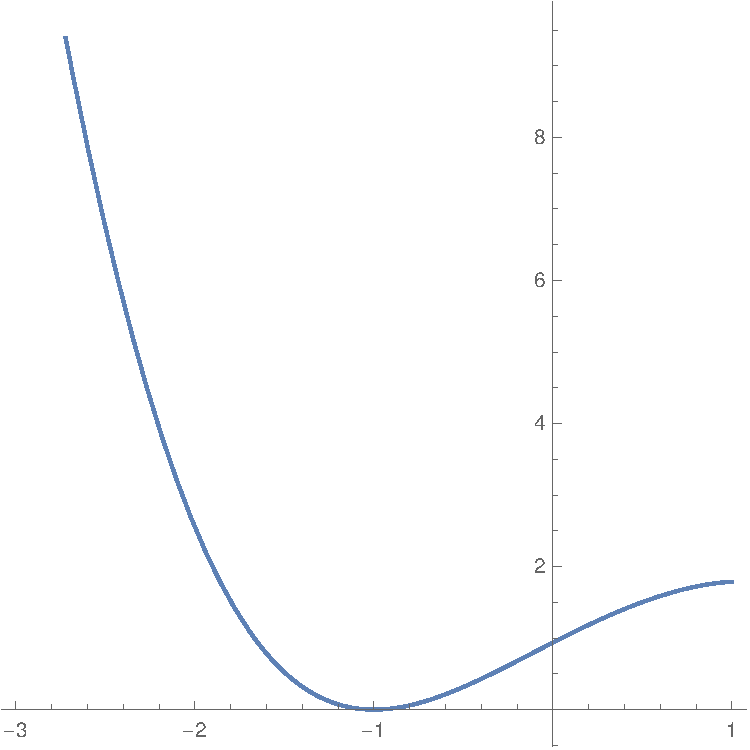
\includegraphics[width=\textwidth]{A8p6.pdf}
		\else
			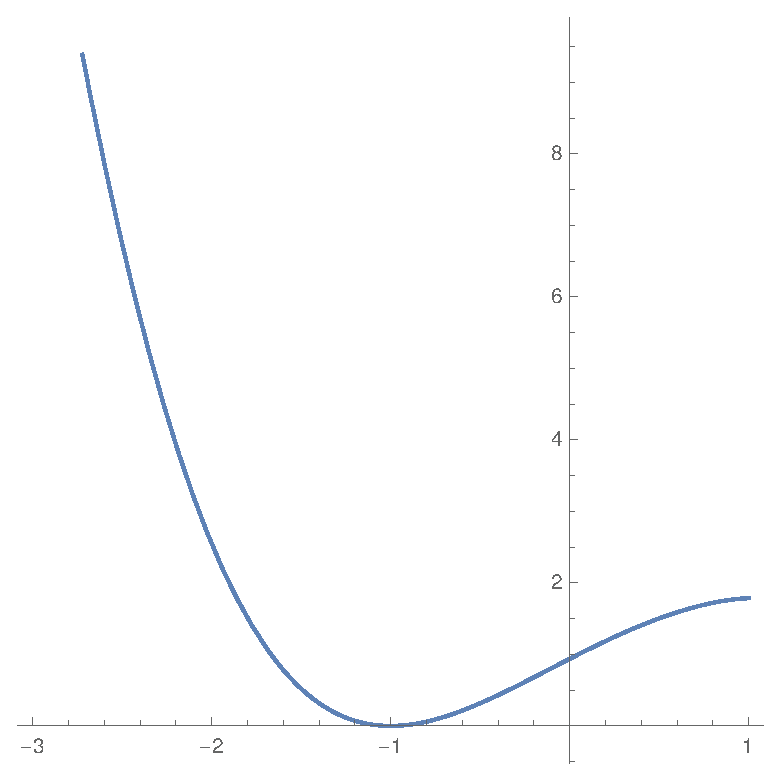
\includegraphics[width=\textwidth]{A8p6.eps}
		\fi
		\caption{Plot of \(g(y) = \min_{x} f(x, y)\)}
		\label{mathematica}
	\end{figure}
\end{proof}


\section{Application}
The length, \(L\), of the longest ladder that can pass around the corner of two corridors depends on the angle \(\alpha\) shown in Figure \ref{ladder}.
\ifnum\webview=1
	\begin{figure}[H]
\else
	\begin{figure}[htbp]
\fi
	\centering
		\ifpdf
			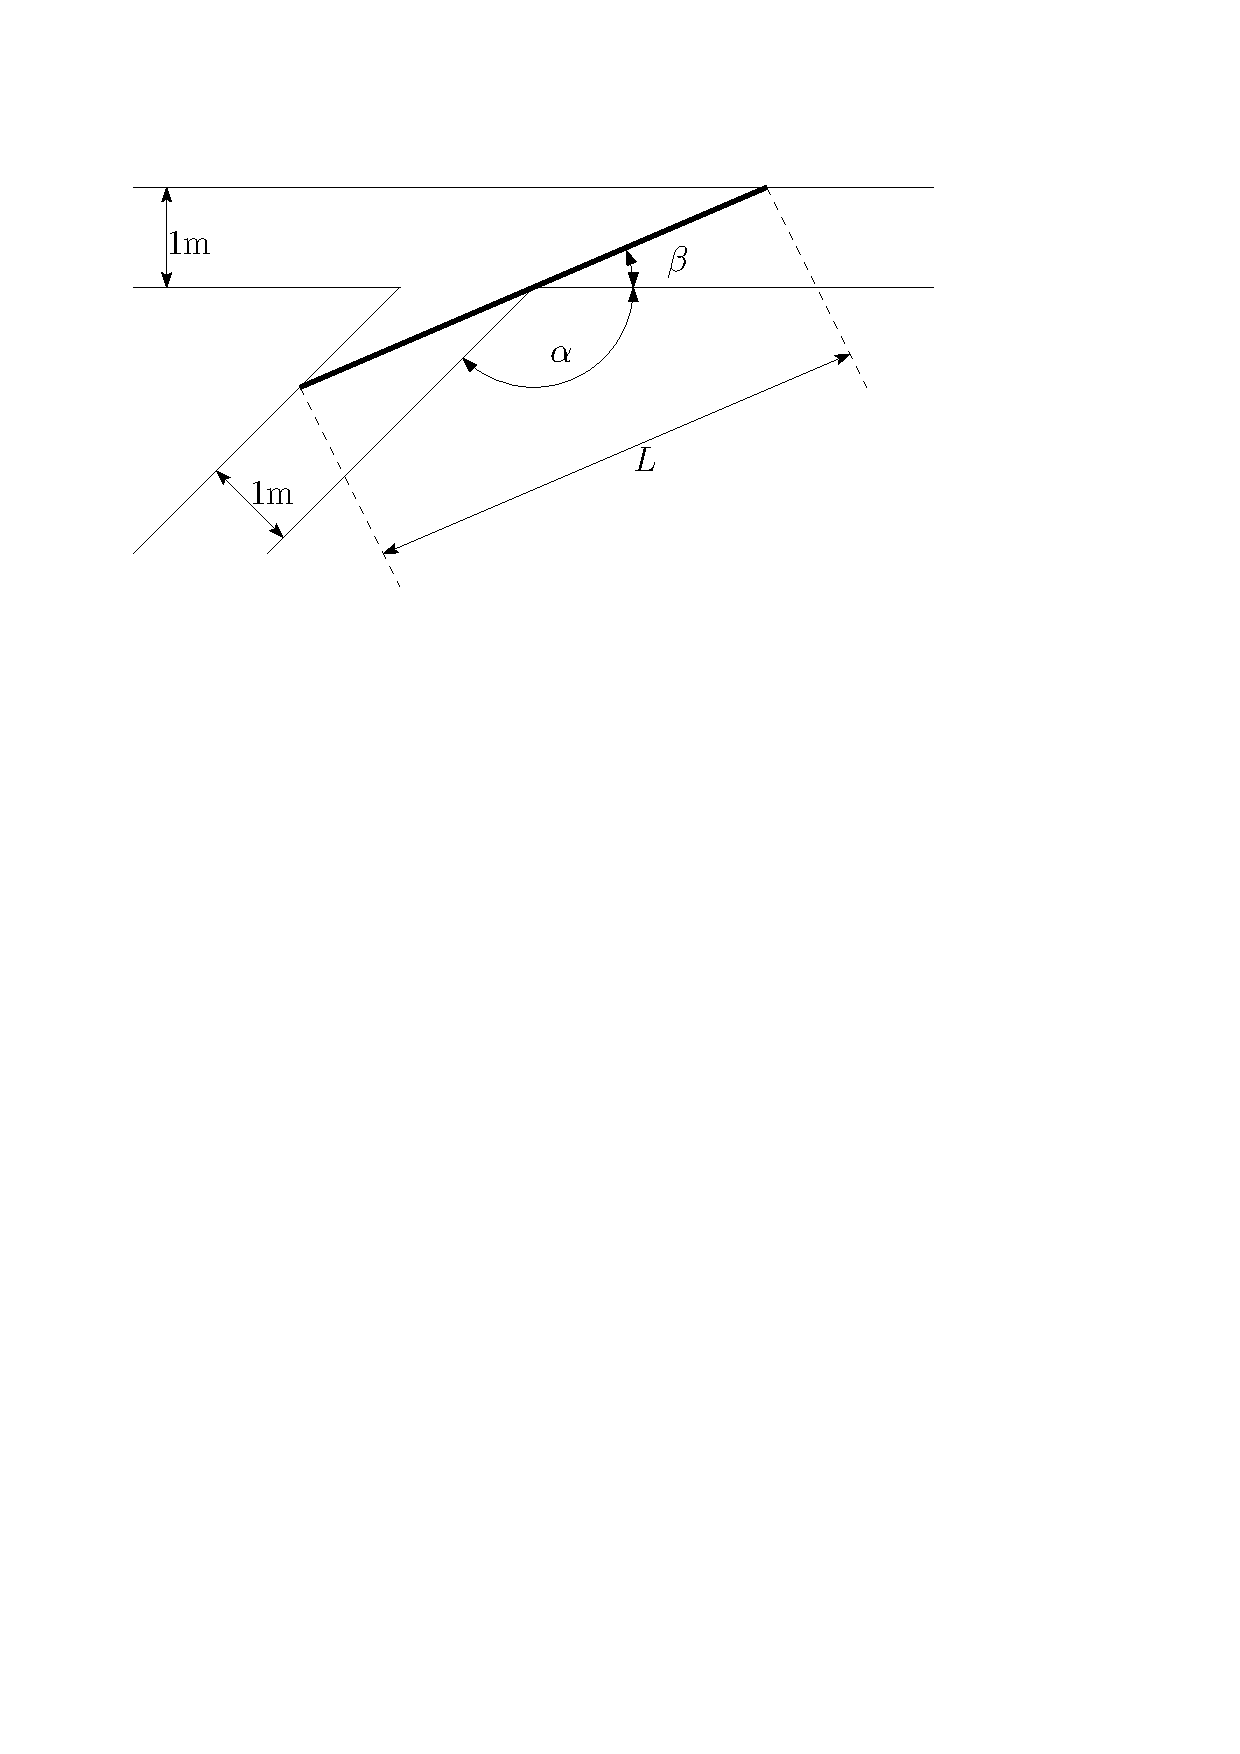
\includegraphics[width=\textwidth]{A8p7.pdf}
		\else
			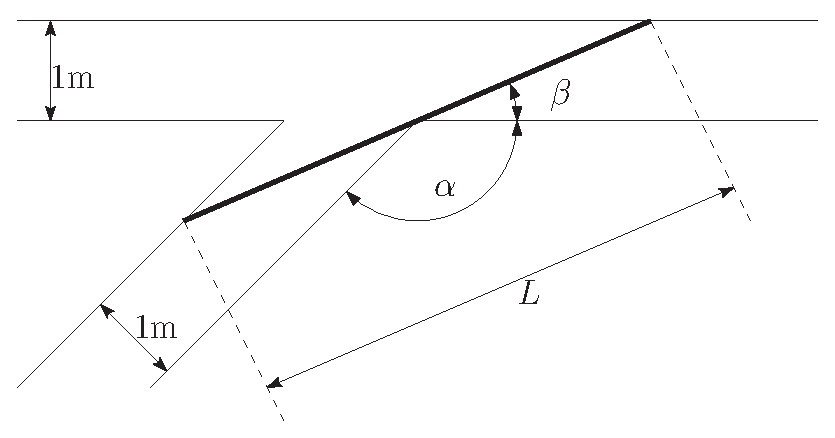
\includegraphics[width=\textwidth]{A8p7.eps}
		\fi
		\caption{Illustration of the situation}
		\label{ladder}
	\end{figure}
Produce a MATLAB\texttrademark\ plot of \(L\) versus \(\alpha\) ranging from \(45^\circ\) to \(135^\circ\) by first solving a minimisation problem using numerical methods that we have discussed so far.
\begin{proof}[Answer]
Observe that
\[ L(\alpha,\beta)=\frac{1}{\sin\beta}+\frac{1}{\sin(\alpha+\beta)}. \]
Regard \(\alpha\) as a parameter, and \(\beta\) as a variable, we need to find
\[ l(\alpha)=\min_{\beta}L(\alpha,\beta). \]
So we require
\[ \partial_\beta L(\alpha,\beta)=0, \quad \partial_{\beta\beta} L(\alpha,\beta)>0. \]
Plug in the function, we find that when
\[ \beta=\frac{\pi-\alpha}{2}, \]
the condition is satisfied.
Thus,
\[ l(\alpha)=L\left(\alpha,\frac{\pi-\alpha}{2}\right)=\frac{1}{\sin\frac{\pi-\alpha}{2}}+\frac{1}{\sin\frac{\pi+\alpha}{2}}. \]
The graph of this function on the desired domain is plotted in Figure \ref{laddersolution}.
\ifnum\webview=1
	\begin{figure}[H]
\else
	\begin{figure}[htbp]
\fi
	\centering
		\ifpdf
			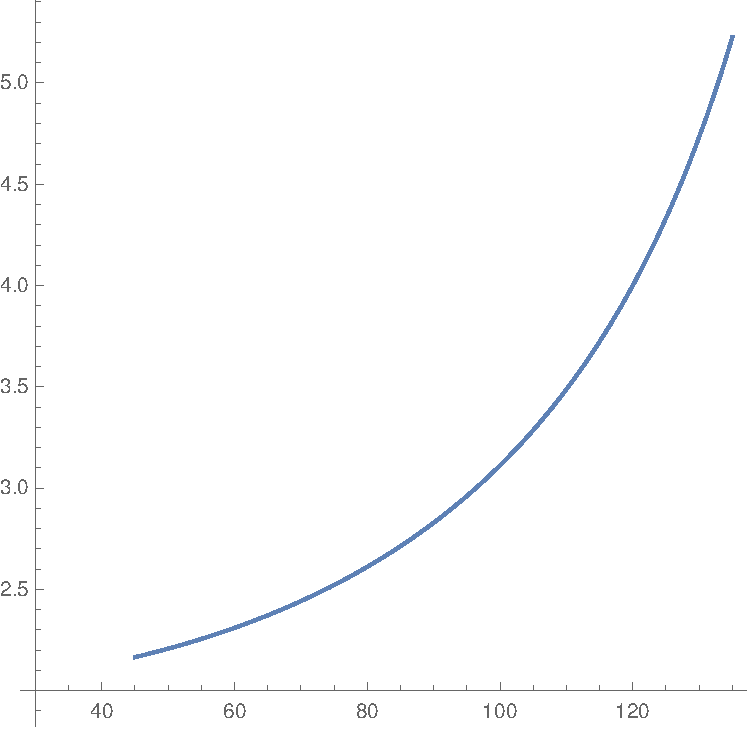
\includegraphics[width=\textwidth]{A8p7s.pdf}
		\else
			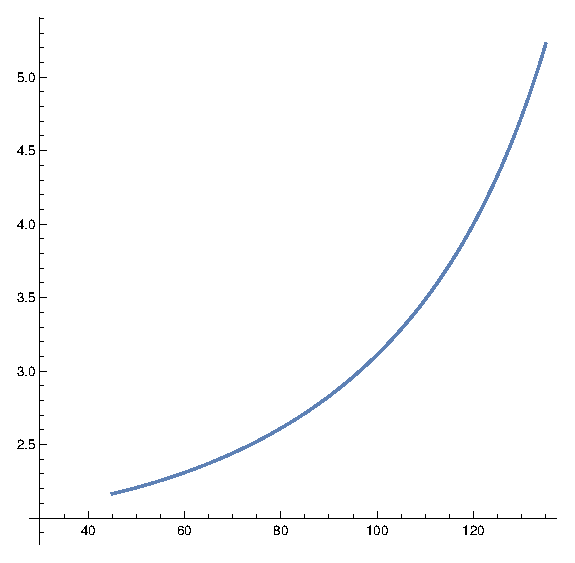
\includegraphics[width=\textwidth]{A8p7s.eps}
		\fi
		\caption{Maximum length to pass the corridors. (\(\beta\) in degrees)}
		\label{laddersolution}
	\end{figure}
\end{proof}


\section{Method of simulated annealing}
A popular global optimization algorithm for difficult functions, especially if there are many local minima, is called the \emph{method of simulated annealing}.
It involves no derivatives or an initial guess that needs to be sufficiently close to the minimum.
Suppose \(f:\R^n \to \R\) has a global minimum at \(x^∗\) and the $k$-iteration \(x_k\) has been computed.
It iterates by the following scheme:
\begin{enumerate}
	\item Generating a number of random points \(u_1, u_2,\cdots, u_m\) in a large neighborhood of \(x_k\).
	\item Computing \(f(u_1), f(u_2),\cdots, f(u_m)\).
	\item Finding the index \(j\) such that \(f(u_j)=\min\{f(u_1), f(u_2),\cdots, f(u_m)\}\).
	\item Assigning \(x_{k+1}=u_j\) if \(f(x_k)>f(u_j)\).
	Otherwise assigning a probability
	\[ p_i=\frac{\exp\{\alpha[f(x_k)-f(u_i)]\}}{\sum_{\ell=1}^{m}\exp\{\alpha[f(x_k)-f(u_\ell)]\}}, \quad \alpha>0, \]
	to \(u_i\) for each \(i=1, \cdots, m\).
	Then making a random choice among \(u_1, u_2,\cdots, u_m\) according to the probabilities \(p_i\) and assigning this randomly chosen \(u_\ell\) to be \(x_{k+1}\).
\end{enumerate}
With some minor modifications, this can be used for function \(Q: \mathcal{X}\to\R\), where \(\mathcal{X}\) is any set.
For example, in the \emph{traveling salesman problem}, \(\mathcal{X}\) is the set of all permutations of a set of integers.
Consider the \emph{Euclidean traveling salesman problem} (ETSP):
given a set of points in \(\R^2\) representing positions of cities on a map, we wish to visit each city exactly once while minimizing the total distance traveled.
\begin{enumerate}
	\item Implement simulated annealing to solve ETSP with different \(\alpha\).
	\item Propose another optimization method to solve ETSP.
	Analyze how its efficiency would compare to that of simulated annealing.
\end{enumerate}

\part{Labs}
\renewcommand{\chaptername}{Lab}
\renewcommand{\thesection}{\arabic{section}}
\titleformat{\section}{\normalfont\Large\bfseries}{Task \thesection}{1em}{}
%!TEX root = ../main.tex
\titleformat{\section}{\normalfont\Large\bfseries}{Task \thesection}{1em}{}
\chapter{Interpolation}
%!TEX root = ../main.tex
\titleformat{\section}{\normalfont\Large\bfseries}{Task \thesection}{1em}{}
\chapter{Intergration}

\section*{Task 1}
In this question, we will investigate the convergence of some common quadrature rules.
\begin{enumerate}[(a)]
	\item Study and write down the output of the following commands.
	\begin{lstlisting}[style=Matlab-editor]
syms x
fsym = symfun(1/(1+25*x^2), x); %Symbolic f
fsym( -1:1:1 )
fano = @(x) 1./(1+25*x.^2); %Anonymous f
fano( -1:1:1 )
exactf = int(fsym,-1,1);
format longE
eval(exactf)
format short
	\end{lstlisting}
	\item Write an M-function to implement the so-called midpoint quadrature rule
	\[ \int_{a}^{b}f(x)\ud x\approx \sum_{k=1}^n(x_k-x_{k-1})f\left(\frac{x_{k-1}+x_k}{2}\right),\]
	where \(a=x_0\) and \(b=x_n\).
	The code for you m-file might look like the following:
	\begin{lstlisting}[style=Matlab-editor]
function quad = midpointquad( f, a, b, n)
%---------------------------------------------
%MIDPOINTQUAD Midpoint Quadrature Rule
% Input
% f integrand
% a, b upper and lower limits of integration
% n the number of equally spaced subintervals
% Output
% quad quadrature value
%
% If f is defined as an M-function use the @ notation to call
% quad=midpointquad(@f,a,b,n)
% If f is defined as an anonymous/symbolic function then simply call
% quad=midpointquad(f,a,b,n)
%---------------------------------------------
xpts = linspace( ??? ) ;
h = ??? ;
xmidpts = zeros(1, ??? );
for i = 1: ???
	xmidpts(i) = ??? ;
end
quad = h * sum ( ??? );
	\end{lstlisting}
	\item Run the following commands and study the output of it.
	\begin{lstlisting}[style=Matlab-editor]
N = 5;
nvec = (2 * 10 .^ (1:1:N));
result = zeros(1, N);
error = zeros(1,N);
for i = 1:N
	result(i) = midpointquad(fano,-1,1,nvec(i));
	error(i) = eval(result(i) - exactf);
end
format longE
T = table( categorical(nvec'), categorical(2./nvec'), result', error', 'VariableNames', {'n' 'h' 'Midpoint' 'Error'})
format short
	\end{lstlisting}
	Use the output to estimate the convergence rate of the midpoint rule in terms of \(h\).
	\item Write an M-function to implement the so-called trapezoidal quadrature rule
	\[ \int_{a}^{b}f(x)\ud x\approx \sum_{k=1}^n(x_k-x_{k-1})\frac{f(x_{k-1})+f(x_k)}{2}, \]
	using equally spaced subintervals, where \(a=x_0\) and \(b=x_n\).
	Name this M-function \texttt{trapezoidalquad}, then estimate the convergence rate of the trapezoidal rule in terms of h using Runge's function.
	\item Write an M-function to implement the so-called Simpson's quadrature rule
	\[ \int_{a}^{b}f(x)\ud x\approx \sum_{k=1}^n\frac{x_k-x_{k-1}}{6}\left[ f(x_{k-1})+4\left(\frac{x_{k-1}+x_k}{2}\right)+f(x_k)\right], \]
	using equally spaced subintervals.
	Name this M-function \texttt{simpsonquad}, then estimate the convergence rate of the Simpson's rule in terms of \(h\) using Runge's function.
	\item Consider applying the midpoint quadrature rule to the following integral
	\[ \int_0^1\ln x\ud x=-1. \]
	Estimate the rate of convergence of the midpoint quadrature rule using this integral.
\end{enumerate}


\section*{Task 2}
In this question, we will test Newton-Cotes, Clenshaw-Curtis, Gaussian quadrature rules.
\begin{enumerate}[(a)]
	\item Use the given M-function \hyperref[newpoly]{newpoly} to construct interpolating polynomials in Newton's form of degree \(n=1,2,3,4,5,10,15,20\) on equally spaced nodes for Gaussian function
	\[ f(x)=e^{x^2} \]
	then integrate the polynomials symbolically over \([-1, 1]\) to approximate
	\[ \int_{-1}^{1}e^{x^2}\ud x. \]
	Note this approach does NOT break \([-1, 1]\) into subintervals.
	\item Repeat part (a), but this time, do it for Runge's function
	\[ \int_{-1}^{1}\frac{1}{1+25x^2}\ud x. \]
	\item Repeat part (b), but this time, do it using Chebyshev nodes instead.
	Study and compare the accuracy of it with the approximation in part (b).
	\item Repeat part (b), but this time, do it using the given M-function \hyperref[fclencurt]{fclencurt} 	and \hyperref[lgwt]{lgwt}, which output the Clenshaw-Curtis and Gauss-Legendre nodes and weights, respectively.
	Compare the accuracy of those two quadrature rules with the approximations in part (b) and part (c).
\end{enumerate}



\section*{Task 3}
This question is to investigate the so-called {\color{blue}degree of exactness} of a quadrature rule.
\begin{enumerate}[(a)]
	\item Run the following commands and study the output of it
	\begin{lstlisting}[style=Matlab-editor]
clear all
syms x
N = 5;
miderror = zeros(1,N);
traperror = zeros(1,N);
simerror = zeros(1,N);
for i = 1:N
	fsym = symfun(i*x^(i-1), x);
	miderror(i) = midpointquad(fsym,0,1,1) - 1;
	traperror(i) = trapezoidalquad(fsym,0,1,1) - 1;
	simerror(i) = simpsonquad(fsym,0,1,1) - 1 ;
end
format long
monomial = {'$1$';'$2x$';'$3x^2$';'$4x^3$';'$5x^4$'};
T = table(monomial , miderror', traperror', simerror', 'VariableNames', {'func' 'MidpointError' 'TrapezoidalError' 'SimpsonError' })
format short
	\end{lstlisting}
	What can you conclude from the output?
	\item Do a similar investigation for Clenshaw-Curtis and Gauss-Legendre.
\end{enumerate}


\section*{Task 4}
This question is to combine and extend what we have learnt about quadrature rules so far.
\begin{enumerate}
	\item Based on Task 1-3, propose an algorithm by writing an M-function that
performs a numerical integration, and test it using the following integral
	\[ \int_{-1}^{1}\frac{1}{1+25x^2}\ud x. \]
	\item  Suggest two additional techniques that can be used to numerically solve the
following integrals, or integrals that have similar features.
	\[ \int_{0}^{\infty}\frac{1}{1+25x^2}\ud x \quad \text{and} \quad \int_{-1}^{1}\sqrt{\left|x-\frac{1}{2}\right|}\ud x . \]

\end{enumerate}
%!TEX root = ../main.tex
\titleformat{\section}{\normalfont\Large\bfseries}{Task \thesection}{1em}{}
\chapter{Root Finding}

%!TEX root = ../main.tex
\chapter{Differential Equations}

\section{}
In this question we compare the convergence of a few methods we have done in class.
\[ \dot{y}=\frac{y+t}{y-t}, \quad y(0)=1. \]
\begin{enumerate}[(a)]
	\item Matlab can solve simple differential equations symbolically.
	For example,
	\begin{lstlisting}[style=Matlab-editor]
equation = 'Dy = (y+t)/(y-t)';
initial = 'y(0) = 1';
y = dsolve(equation, initial, 't');
pretty(y)
x = linspace( 0, 1, 20);
z = eval(vectorize(y));
plot(x,z)
	\end{lstlisting}
	Run the above commands and write down the exact solution below.
	\item Study and use the M-function \hyperref[butcher]{butcher} and \hyperref[euler]{euler} to estimate the convergence rate of Euler's method for the above IVP over the interval \([0, 1]\).
	In addition, compute the error as the difference between your approximation and the exact solution at \(t = 1\).
	\item Repeat part (b), but this time do it for Heun's method.
	The M-function \hyperref[heun]{heun} is given.
	\item Repeat to part (b), but this time do it for Aadms-Bashforth's method.
	The M-function \hyperref[ab2]{ab2} is given.
	\item Repeat to part (b), but this time do it for the classic 4-order Runge Kutta's method.
	The M-function \hyperref[rk4]{rk4} is given.
	\item Repeat to part (b), but this time do it for the classic 4-order Taylor's method.
	The M-function \hyperref[taylor]{taylor} is given.
\end{enumerate}


\section{}
Matlab has its implementation of Runge-Kutta.
This question looks at the build-in functions {\color{blue}ode23} and {\color{blue}ode45}, which implement versions of 2nd/3rd-order Runge-Kutta and 4th/5th-order Runge Kutta, respectively.
\begin{enumerate}[(a)]
	\item ) Study and use {\color{blue}ode23} to solve the following
	\[ \dot{y}=\frac{y+t}{y-t}, \quad y(0)=1. \]
	Compare and comment the convergence with the methods we considered in Task 1.
	\item Write an M-function for the vector-valued function
	\[ \Phi(t,x)=\begin{bmatrix} 10(x_2-x_1) \\ 28x_1-x_2-x_1x_3 \\ -8/3x_3+x_2x_2 \end{bmatrix} \]
	The input of your function shall be a scalar \(t\) and a vector in \(\R^3\).
	The output of your function shall be a column vector.
	\item  Study and use {\color{blue}ode45} to solve the following IVP over \([0, 20]\).
	\[ \dot{x}=\Phi(x), \quad x(0)=\begin{bmatrix} -8 \\ 8 \\ 27 \end{bmatrix}. \]
	\item 
\end{enumerate}

\part{Projects}
\renewcommand{\chaptername}{Projects}
\titleformat{\section}{\normalfont\Large\bfseries}{\thesection}{1em}{}
%!TEX root = main.tex
\titleformat{\section}{\normalfont\large\bfseries}{\thesection}{1em}{}
\renewcommand{\chaptername}{Project}
\renewcommand{\thesection}{\arabic{section}}



\chapter{Linear Prediction of Speech}
\begin{center}
Guangting Yu, University of Michigan - Shanghai Jiao Tong University Joint Institute, Minhang, Shanghai, 200135, China
\end{center}


\section*{Abstract}
This paper talks about numerical methods.



\section{Background}
Speech production is the result of an excitation signal generated by the contraction of the lungs when they expel air.\cite{dutoit}
It is then modified by resonances when passing through the trachea, the vocal cords, the mouth cavity, as well as various muscles.\cite{tam59}
The excitation signal is either created by the opening and closing of the vocal cords, or by a continuous flow of air.\cite{gtm181}
Introduced in the early 1960s by Fant, \textit{the source-filter} model assumes that the glottis and vocal tract are fully uncoupled.\cite{corless}
This initial idea was reused to develop the \textit{Linear Predictive} (LP) model for speech production.\cite{tam39}

In this model the speech signal is the output \(y[n]\) of an \textit{all-pole filter}\footnote{A filter whose frequency response function goes infinite at specific frequencies} \(1/A(z)\) excited by \(x[n]\).\cite{golan}
Calling \(Y(z)\) and \(X(z)\) the Z-transform of the speech and excitation, respectively, the model is described by\cite{utm}
\begin{equation}
Y(z)=\frac{X(z)}{1-\sum_{i=0}^p a_i z^{-i}}=\frac{X(z)}{A_p}.
\end{equation}

Applying the inverse Z-transform to this equation we observe that the speech can be linearly predicted from the previous $p$ samples and some excitation:
\begin{equation}
y[n] = x[n]+\sum_{i=1}^p a_i y[n-i].
\end{equation}


Our goal is to explain as much as possible of \(y[n]\) through the $a_i$ , \textit{i.e.}, we look at \(x[n]\) as an error, and we strive at rendering it as small and simple as possible.\cite{gtm135}
For the sake of clarity we therefore rename \(x[n]\) into \(e[n]\).\cite{cc12}
The question we want to answer is how to select the $a_i$ such as to minimize the energy
\begin{equation}
E=\sum_{m=-\infty}^\infty e^2[m].
\end{equation}


\begin{enumerate}
	\item Show that
	\begin{equation}
	\sum_{m=-\infty}^{\infty} y[m]y[m-i]=\sum_{i=1}^p a_i\sum_{m=-\infty}^{\infty} y[m-i]y[m-i], \quad i=1,\cdots,p.
	\end{equation}
	Since those sums are infinite they cannot be computed, and as such need to be truncated.\cite{karris}
	This can be achieved by applying the covariance method, which consists in windowing the error
	\begin{equation}
	E_n=\sum_{m=n}^{n+N-1}\left(y[m]-\sum_{i=1}^p a_i y[m-k] \right)^2.
	\end{equation}
	\item Prove that
	\begin{align*}
	\phi_n(k,0)&=\sum_{i=0}^p a_i\phi_n(k,i), \\
	\phi_n(k,i)&=\sum_{m=n}^{n+N-1} y[m-k]y[m-k].
	\end{align*}
	\item Conclude that
	\begin{equation}
	\begin{pmatrix} \phi(1,0)\\ \vdots \\ \phi(p,0) \end{pmatrix}=\begin{pmatrix} \phi(1,1) & \cdots & \phi(1,p) \\ \vdots & & \vdots \\ \phi(p,1) & \cdots & \phi(p,p) \end{pmatrix}\begin{pmatrix} a_1 \\ \vdots \\ a_p \end{pmatrix}.
	\end{equation}
	Determining the optimal value for the \(a_i, 1\leq i\leq p\), implies inverting the matrix $\Phi$.
	This can be achieved through Cholesky decomposition.\cite{gtm216,gtm135}
\end{enumerate}


\section{Linear algebra}




\begin{definition}[Hermitian matrix]
A Matrix \(A\in\C^{n\times n}\) is \emph{Hermitian} if it is equal to the conjugate transpose of itself, \textit{i.e.},
\begin{equation*}
A=\bar{A}^T.
\end{equation*}
\end{definition}


\begin{definition}[Eigenvalues ad eigenvectors]
A number \(\lambda\in\C\) is called an \emph{eigenvalue} of \(A\in\C^{n\times n}\) if there exists \(v\in\C^n\) such that \(v\neq0\) and
\begin{equation*}
Av=\lambda v.
\end{equation*}
Such a vector $v$ is called an \emph{eigenvector}.
\end{definition}


\begin{definition}[Spectrum]
The \emph{spectrum} of \(A\in\C^{n\times n}\), denoted as \(\sigma_A\), is the set of all the eigenvalues of $A$, \textit{i.e.},
\begin{equation*}
\sigma_A\coloneqq\Set{\lambda}{\lambda \text{ is a eigenvalue of }A}
\end{equation*}
\end{definition}


\begin{definition}[Spectrum radius]
The \emph{spectrum radius} of \(A\in\C^{n\times n}\), denoted as \(\rho(A)\), is the largest absolute value of all its eigenvalues, \textit{i.e.},
\begin{equation*}
\rho(A)\coloneqq\max_{\lambda\in\sigma_A}|\lambda|.
\end{equation*}
\end{definition}


\begin{theorem}
If a matrix \(A\in\C^{n\times n}\) is Hermitian, then \(\sigma_A\subset\R\).
\end{theorem}
\begin{proof}
Take any eigenvalue \(\lambda\in\sigma_A\) and its corresponding eigenvector \(v\in\C^n\).
By definition,
\begin{equation}
Av=\lambda v.
\end{equation}
Multiply both sides by the conjugate transpose of $v$,
\begin{equation}\label{hermitianproof}
\bar{v}^T Av=\lambda \bar{v}^T v.
\end{equation}
The left hand side of the equation has the conjugate transpose
\begin{equation}
\overline{\bar{v}^T Av}^T=\bar{v}^T\bar{A}^T v.
\end{equation}
Since $A$ is Hermitian, we plug in \(\bar{A}^T=A\) on the right hand side and
\begin{equation}
\overline{\bar{v}^T Av}^T=\bar{v}^TA v,
\end{equation}
which implies that \(\bar{v}^T Av\) is also Hermitian.
Furthermore, \(\bar{v}^T Av\in\C^{1\times1}\) implies that it is a real number.
Then, according to equation \ref{hermitianproof}
\begin{equation}
\lambda=\frac{\bar{v}^T Av}{\bar{v}^T v}.
\end{equation}
The denominator is the inner product of $v$ with itself defined on \(\C^n\), so \(\bar{v}^T v\in\R_*^+\) since \(v\neq0\).
Both the numerator and the denominator are real, so the quotient $\lambda$ is also real.
Since $\lambda$ is arbitrarily selected from \(\sigma_A\), all elements in \(\sigma_A\) are real.
Furthermore, \(sigma_A\) has at most $n$ elements, so it is a proper subset of 
\end{proof}



\part{External Resources}
\renewcommand{\chaptername}{External Resource}
\lstset{xleftmargin=.05\textwidth, xrightmargin=0.01\textwidth}
%!TEX root = main.tex
\chapter{MATLAB\texttrademark\ Codes}

\section{Butcher's method\label{butcher}}
\lstinputlisting[style=Matlab-editor]{mcode/butcher.m}

\section{Euler's method\label{euler}}
\lstinputlisting[style=Matlab-editor]{mcode/euler.m}

\section{Heun's method\label{heun}}
\lstinputlisting[style=Matlab-editor]{mcode/heun.m}

\section{Aadms-Bashforth's method\label{ab2}}
\lstinputlisting[style=Matlab-editor]{mcode/ab2.m}

\section{4-order Runge Kutta's method\label{rk4}}
\lstinputlisting[style=Matlab-editor]{mcode/rk4.m}

\section{4-order Taylor's method\label{taylor}}
\lstinputlisting[style=Matlab-editor]{mcode/taylor.m}

\printbibliography
\end{document}
